\documentclass[14pt]{extarticle}

\usepackage[table]{xcolor}
\usepackage{amsmath,mathtools,amsfonts,amsthm,amssymb,hyperref,wasysym,pifont,bm}
\usepackage{parskip,geometry,latexsym,bookmark,mathtools,float,cancel,tcolorbox}

% for the Power set P
\usepackage[mathscr]{euscript}
\let\euscr\mathscr 
\let\mathscr\relax
\usepackage[scr]{rsfso}
\newcommand{\ps}{\mathscr{P}}

\newtheorem{defn}{Definition}
\newtheorem{thm}{Theorem}
\newtheorem{claim}{Claim}
\newtheorem{lemma}{Lemma}

\renewcommand{\arraystretch}{1.3}

\newcommand{\es}{\varnothing}
\newcommand{\dps}{\displaystyle}
\newcommand{\fbl}{\underline{\hspace{1cm}}\,\,}
\newcommand{\R}{\mathbb{R}}
\newcommand{\Z}{\mathbb{Z}}
\newcommand{\from}{\leftarrow}
\newcommand{\true}{{\bf t}}
\newcommand{\false}{{\bf c}}
\newcommand{\bic}{\leftrightarrow}
\newcommand{\base}[1]{{\color{cyan}\subseteq1}}
\newcommand{\floor}[1]{{\left\lfloor\subseteq1\right\rfloor}}
\newcommand{\ceil}[1]{{\lceil\subseteq1\rceil}}
\newcommand{\da}{\downarrow}
\newcommand{\fa}{\forall}
\newcommand{\te}{\exists}
\newcommand{\cy}{\color{cyan}}

\newcommand{\colsq}[1]{{\color{\subseteq1} $\blacksquare$}}

\newcommand\Ccancel[2][black]{\renewcommand\CancelColor{\color{\subseteq1}}\cancel{\subseteq2}}
\newcommand\Cbcancel[2][black]{\renewcommand\CancelColor{\color{\subseteq1}}\bcancel{\subseteq2}}

\hypersetup{colorlinks,allcolors=blue,linktoc=all}
\geometry{a4paper}
\geometry{margin=0.42in}

\title{Chapter 6 Solutions, Susanna Epp Discrete Math 5th Edition}

\author{https://github.com/spamegg1}

\begin{document}
\maketitle
\tableofcontents

\section{Exercise Set 6.1}

\subsection{Exercise 1}
In each of (a)-(f), answer the following questions: Is \(A \subseteq B\)? Is \(B \subseteq A\)? 
Is either $A$ or $B$ a proper subset of the other?

\subsubsection{(a)}
\(A = \{2, \{2\}, (\sqrt{2})^2\}, B = \{2, \{2\}, \{\{2\}\}\}\)

\begin{proof}
\(A = \{2, \{2\}, (\sqrt{2})^2\} = \{2, \{2\}, 2\} = \{2, \{2\}\}\), so \(A \subseteq B\) because every element of $A$
is in $B$, but \(B \nsubseteq A\) because \(\{\{2\}\} \in B\) but \(\{\{2\}\} \notin A\). Thus $A$ is a proper subset of $B$.
\end{proof}

\subsubsection{(b)}
\(A = \{3, \sqrt{5^2 - 4^2}, 24 \mod 7\}, B = \{8 \mod 5\}\)

\begin{proof}
\(A = \{3, \sqrt{5^2 - 4^2}, 24 \mod 7\} = \{3, 3, 3\} = \{3\}, B = \{8 \mod 5\} = \{3\}\). So $A = B$, which means
both \(A \subseteq B\) and \(B \subseteq A\).
\end{proof}

\subsubsection{(c)}
\(A = \{\{1, 2\}, \{2, 3\}\}, B = \{1, 2, 3\}\)

\begin{proof}
\(A \nsubseteq B\) because $\{1, 2\} \in A$ but $\{1, 2\} \notin B$.
\(B \nsubseteq A\) because $1 \in B$ but $1 \notin A$.
\end{proof}

\subsubsection{(d)}
\(A = \{a, b, c\}, B = \{\{a\}, \{b\}, \{c\}\}\)

\begin{proof}
\(A \nsubseteq B\) because $a \in A$ but $a \notin B$.
\(B \nsubseteq A\) because $\{a\} \in B$ but $\{a\} \notin A$.
\end{proof}

\subsubsection{(e)}
\(A = \{\sqrt{16}, \{4\}\}, B = \{4\}\)

\begin{proof}
\(A = \{\sqrt{16}, \{4\}\} = \{4, \{4\}\}\). 
\(B \subseteq A\) because $4$ is the only element of $B$ and $4 \in A$.
\(A \nsubseteq B\) because \(\{4\} \in A\) but \(\{4\} \notin B\).
\end{proof}

\subsubsection{(f)}
\(A = \{x \in \R \, | \, \cos(x) \in \Z\}, B = \{x \in \R \, | \, \sin(x) \in \Z\}\)

\begin{proof}
From trigonometry we know that \(\cos(x)\) and \(\sin(x)\) have the only integer values $-1, 0$ and $1$. We also know that 

\(\cos(x) = -1\) if and only if \(x = \pi + 2n\pi\) for some integer $n \in \Z$ 
(\(\ldots, -3\pi, -\pi, \pi, 3\pi, \ldots\)),

\(\cos(x) = 0\) if and only if \(x = \frac{\pi}{2} + n\pi\) for some integer $n \in \Z$ 
(\(\ldots, -\frac{3\pi}{2}, -\frac{\pi}{2}, \frac{\pi}{2}, \frac{3\pi}{2}, \ldots\)),

\(\cos(x) = 1\) if and only if \(x = 2n\pi\) for some integer $n \in \Z$ 
(\(\ldots, -4\pi, -2\pi, 0, 2\pi, 4\pi, \ldots\)),

\(\sin(x) = -1\) if and only if \(x = -\frac{\pi}{2} + 2n\pi\) for some integer $n \in \Z$
(\(\ldots, -\frac{5\pi}{2}, -\frac{\pi}{2}, \frac{3\pi}{2}, \frac{7\pi}{2}, \ldots\)),

\(\sin(x) = 0\) if and only if \(x = n\pi\) for some integer $n \in \Z$,
(\(\ldots, -2\pi, -\pi, 0, \pi, 2\pi, \ldots\)),

\(\sin(x) = 1\) if and only if \(x = \frac{\pi}{2} + 2n\pi\) for some integer $n \in \Z$
(\(\ldots, -\frac{7\pi}{2}, -\frac{3\pi}{2}, \frac{\pi}{2}, \frac{5\pi}{2}, \ldots\)).

So:
\[
A = \{\cdots, -\frac{5\pi}{2}, -2\pi, -\frac{3\pi}{2}, -\pi, -\frac{\pi}{2}, 0, \frac{\pi}{2}, \pi, \frac{3\pi}{2}, 2\pi, \frac{5\pi}{2}, \cdots\}
\]
and
\[
B = \{\cdots, -\frac{5\pi}{2}, -2\pi, -\frac{3\pi}{2}, -\pi, -\frac{\pi}{2}, 0, \frac{\pi}{2}, \pi, \frac{3\pi}{2}, 2\pi, \frac{5\pi}{2}, \cdots\}
\]
so $A = B$.
\end{proof}

\subsection{Exercise 2}
Complete the proof from Example 6.1.3: 
Prove that \(B \subseteq A\) where \(A = \{m \in \Z \, | \, m = 2a \text{ for some integer } a\}\) and 
\(B = \{n \in \Z \, | \, n = 2b - 2 \text{ for some integer } b\}\)

\begin{proof}
{\bf Proof That $B \subseteq A$:} Suppose $x$ is a particular but arbitrarily chosen element of $B$. 

{\it [We must show that $x \in A$. By definition of $A$, this means we must show that $x = 2 \cdot$(some integer).]}

By definition of $B$, there is an integer $b$ such that \(x = 2b - 2\). 

{\it [Given that \(x = 2b - 2\), can $x$ also be expressed as $2 \cdot$ (some integer)? That is, is there an integer, say, a, such that \(2b - 2 = 2a\)? Solve for $a$ to obtain \(a = b - 1\). Check to see if this works.]}

Let \(a = b - 1\). 

{\it [First check that a is an integer.]} 

We know that $a$ is an integer because it is a difference of integers. 

{\it [Then check that \(x = 2a\).]}

By substitution, \(2a = 2(b - 1) = 2b - 2 = x\). Thus, by 
definition of $A$, $x$ is an element of $A$, {\it [as was to be shown]}.
\end{proof}

\subsection{Exercise 3}
Let sets $R, S$, and $T$ be defined as follows:
\begin{center}
\begin{tabular}{rcl}
$R$ & = & \(\{x \in \Z \, | \, x \text{ is divisible by 2} \}\) \\
$S$ & = & \(\{y \in \Z \, | \, y \text{ is divisible by 3} \}\) \\
$T$ & = & \(\{z \in \Z \, | \, z \text{ is divisible by 6} \}\)
\end{tabular}
\end{center}
Prove or disprove each of the following statements.

\subsubsection{(a)}
\(R \subseteq T\)

\begin{proof}
\(R \nsubseteq T\) because there are elements in $R$ that are not in $T$. For example, the number $2$ is in $R$ but 
$2$ is not in $T$ since $2$ is not divisible by $6$.
\end{proof}

\subsubsection{(b)}
\(T \subseteq R\)

\begin{proof}
\(T \subseteq R\) because every element in $T$ is in $R$ since every integer divisible by 6 is divisible by 2. To 
see why this is so, suppose $n$ is any integer that is divisible by 6. Then $n = 6m$ for some integer $m$. Since 
\(6m = 2(3m)\) and since $3m$ is an integer (being a product of integers), it follows that \(n = 2 \cdot \)(some 
integer), and, hence, that $n$ is divisible by 2.
\end{proof}

\subsubsection{(c)}
\(T \subseteq S\)

\begin{proof}
\(T \subseteq S\) because every element in $T$ is in $S$ since every integer divisible by 6 is divisible by 3. To 
see why this is so, suppose $n$ is any integer that is divisible by 6. Then $n = 6m$ for some integer $m$. Since 
\(6m = 3(2m)\) and since $2m$ is an integer (being a product of integers), it follows that \(n = 3 \cdot \)(some 
integer), and, hence, that $n$ is divisible by 3.
\end{proof}

\subsection{Exercise 4}
Let \(A = \{n \in \Z \, | \, n = 5r \text{ for some integer } r\}\) and 

\(B = \{m \in \Z \, | \, m = 20s \text{ for some integer } s\}\). Prove or disprove each of the following statements.

\subsubsection{(a)}
\(A \subseteq B\)

\begin{proof}
\(A \nsubseteq B\) because $5 \in A$ but $5 \notin B$.
\end{proof}

\subsubsection{(b)}
\(B \subseteq A\)

\begin{proof}
\(B \subseteq A\) is true. Suppose $m \in B$. Then $m = 20s$ for some integer $s$. So $m = 20s = 5(4s)$ where $4s$ 
is an integer, therefore $m \in A$.
\end{proof}

\subsection{Exercise 5}
Let \(C = \{n \in \Z \, | \, n = 6r-5 \text{ for some integer } r\}\) and \(D = \{m \in \Z \, | \, m = 3s+1 
\text{ for some integer } s\}\). Prove or disprove each of the following statements.

\subsubsection{(a)}
\(C \subseteq D\)

\begin{proof}
\(C \subseteq D\) because every element in $C$ is in $D$. To see why this is so, suppose $n$ is any element of $C$. 
Then \(n = 6r - 5\) for some integer $r$. Let \(s = 2r - 2\). Then $s$ is an integer (because products and 
differences of integers are integers), and \(3s + 1 = 3(2r - 2) + 1 = 6r - 6 + 1 = 6r - 5\), which equals $n$. Thus 
$n$ satisfies the condition for being in $D$. Hence, every element in $C$ is in $D$.
\end{proof}

\subsubsection{(b)}
\(D \subseteq C\)

\begin{proof}
\(D \nsubseteq C\) because there are elements of $D$ that are not in $C$. For example, 4 is in $D$ because 
\(4 = 3 \cdot 1 + 1\). But 4 is not in $C$ because if it were, then \(4 = 6r - 5\) for some integer $r$, which would 
imply that \(9 = 6r\), or, equivalently, that \(r = 3/2\), and this contradicts the fact that $r$ is an integer.
\end{proof}


\subsection{Exercise 6}
Let \(A = \{x \in \Z \, | \, x = 5a+2 \text{ for some integer } a\}\), 

\(B = \{y \in \Z \, | \, y = 10b-3 \text{ for some integer } b\}\) and 

\(D = \{z \in \Z \, | \, z = 10c+7 \text{ for some integer } c\}\). 
Prove or disprove each of the following statements.

\subsubsection{(a)}
\(A \subseteq B\)

\begin{proof}
\(A \nsubseteq B\) because \(2 \in A\) because \(2 = 5 \cdot 0 + 2\), but \(2 \notin B\). To see this, argue by
contradiction and assume \(2 \in B\). So \(2 = 10b - 3\) for some integer $b$. So \(5 = 10b\) and \(b = 1/2\) is an
integer, a contradiction. Therefore our supposition was false and \(2 \notin B\).
\end{proof}

\subsubsection{(b)}
\(B \subseteq A\)

\begin{proof}
Suppose \(y \in B\). Then \(y = 10b - 3\) for some integer $b$. Then \(y = 10b - 5 + 5 - 3 = 5(b-2) + 2\) where $b-2$
is an integer. Let \(a = b-2\). Therefore \(y = 5a + 2\) for some integer $a$, therefore \(y \in A\). 
This proves \(B \subseteq A\).
\end{proof}

\subsubsection{(c)}
$B = C$

\begin{proof}
{\bf Sketch of proof that \(B \subseteq C\):} If $r$ is any element of $B$ then there is an integer $b$ such that 
\(r = 10b - 3\). To show that $r$ is in $C$, you must show that there is an integer $c$ such that \(r = 10c + 7\). In 
scratch work, assume that $c$ exists and use the information that \(10b - 3\) would have to equal 
\(10c + 7\) to deduce the only possible value for $c$. Then show that this value is (1) an integer and (2) satisfies 
the equation \(r = 10c + 7\), which will allow you to conclude that $r$ is an element of $C$.

{\bf Sketch of proof that \(C \subseteq B\):} If $s$ is any element of $C$ then there is an integer $c$ such that 
\(s = 10c + 7\). To show that $s$ is in $B$, you must show that there is an integer $b$ such that \(s = 10c - 3\). In 
scratch work, assume that $b$ exists and use the information that \(10c + 7\) would have to equal 
\(10b - 3\) to deduce the only possible value for $b$. Then show that this value is (1) an integer and (2) satisfies 
the equation \(s = 10b - 3\), which will allow you to conclude that $s$ is an element of $B$.
\end{proof}

\subsection{Exercise 7}
Let \(A = \{x \in \Z \, | \, x = 6a+4 \text{ for some integer } a\}\), 

\(B = \{y \in \Z \, | \, y = 18b-2 \text{ 
for some integer } b\}\) and 

\(D = \{z \in \Z \, | \, z = 18c+16 \text{ for some integer } c\}\). 
Prove or disprove each of the following statements.

\subsubsection{(a)}
\(A \subseteq B\)

\begin{proof}
\(A \nsubseteq B\) because $10 \in A$ but $10 \notin B$. To see this, argue by contradiction and assume $10 \in B$.
Then \(10 = 18b-2\) for some integer $b$. Then \(12 = 18b\) and \(b = 12/18 = 2/3\), which is not an integer,
contradiction. Therefore our supposition was false and $10 \notin B$.
\end{proof}

\subsubsection{(b)}
\(B \subseteq A\)

\begin{proof}
Suppose $y \in B$. Then \(y = 18b-2\) for some integer $b$. Then \(y = 18b-6+6-2 = 6(3b-1) + 4\) where $3b-1$ is an 
integer. Let $a = 3b-1$. So \(y = 6a + 4\) for some integer $a$, therefore $y \in A$. This proves \(B \subseteq A\).
\end{proof}

\subsubsection{(c)}
$B = C$

\begin{proof}
Suppose $y \in B$. Then \(y = 18b-2\) for some integer $b$. Then \(y = 18b-18+18-2 = 18(b-1) + 16\) where $b-1$ is an 
integer. Let $c = b-1$. So \(y = 18c + 16\) for some integer $c$, therefore $y \in C$. This proves \(B \subseteq C\).

Suppose $z \in C$. Then \(z = 18c+16\) for some integer $c$. Then \(z = 18c+18-18+16 = 18(c+1) -2\) where $c+1$ is an integer. Let $b = c+1$. So \(z = 18b -2\) for some integer $b$, therefore $z \in B$. This proves \(C \subseteq B\).
\end{proof}

\subsection{Exercise 8}
Write in words how to read each of the following out loud. Then write each set using the symbols for union, 
intersection, set difference, or set complement.

\subsubsection{(a)}
\(\{x \in U \, | \, x \in A \text{ and } x \in B\}\)

\begin{proof}
{\it In words:} The set of all $x$ in $U$ such that $x$ is in $A$ and $x$ is in $B$.

{\it In symbolic notation:} \(A \cap B\).
\end{proof}

\subsubsection{(b)}
\(\{x \in U \, | \, x \in A \text{ or } x \in B\}\)

\begin{proof}
{\it In words:} The set of all $x$ in $U$ such that $x$ is in $A$ or $x$ is in $B$.

{\it In symbolic notation:} \(A \cup B\).
\end{proof}

\subsubsection{(c)}
\(\{x \in U \, | \, x \in A \text{ and } x \notin B\}\)

\begin{proof}
{\it In words:} The set of all $x$ in $U$ such that $x$ is in $A$ and $x$ is not in $B$.

{\it In symbolic notation:} \(A - B\).
\end{proof}

\subsubsection{(d)}
\(\{x \in U \, | \, x \notin A\}\)

\begin{proof}
{\it In words:} The set of all $x$ in $U$ such that $x$ is not in $A$.

{\it In symbolic notation:} \(A^c\).
\end{proof}

\subsection{Exercise 9}
Complete the following sentences without using the symbols \(\cup, \cap\), or $-$.

\subsubsection{(a)}
\(x \notin A \cup B\) if, and only if, \fbl.

\begin{proof}
\(x \notin A\) and \(x \notin B\)
\end{proof}

\subsubsection{(b)}
\(x \notin A \cap B\) if, and only if, \fbl.

\begin{proof}
\(x \notin A\) or \(x \notin B\)
\end{proof}

\subsubsection{(c)}
\(x \notin A - B\) if, and only if, \fbl.

\begin{proof}
\(x \notin A\) or \(x \in B\)
\end{proof}

\subsection{Exercise 10}
Let \(A = \{1, 3, 5, 7, 9\}\), \(B = \{3, 6, 9\}\), and \(C = \{2, 4, 6, 8\}\). Find each of the following:

\subsubsection{(a)}
\(A \cup B\)

\begin{proof}
\(A \cup B = \{1, 3, 5, 6, 7, 9\}\)
\end{proof}

\subsubsection{(b)}
\(A \cap B\)

\begin{proof}
\(A \cap B = \{3, 9\}\)
\end{proof}

\subsubsection{(c)}
\(A \cup C\)

\begin{proof}
\(A \cup C = \{1, 2, 3, 4, 5, 6, 7, 8, 9\}\)
\end{proof}

\subsubsection{(d)}
\(A \cap C\)

\begin{proof}
\(A \cap C = \es\)
\end{proof}

\subsubsection{(e)}
\(A - B\)

\begin{proof}
\(A - B = \{1, 5, 7\}\)
\end{proof}

\subsubsection{(f)}
\(B - A\)

\begin{proof}
\(B - A = \{6\}\)
\end{proof}

\subsubsection{(g)}
\(B \cup C\)

\begin{proof}
\(B \cup C = \{2, 3, 4, 6, 8, 9\}\)
\end{proof}

\subsubsection{(h)}
\(B \cap C\)

\begin{proof}
\(B \cap C = \{6\}\)
\end{proof}

\subsection{Exercise 11}
Let the universal set be $\R$, the set of all real numbers, and let \(A = \{x \in \R \,|\, 0 < x \leq 2\}\), \(B = \{x 
\in \R \, | \, 1 \leq x < 4\}\), and \(C = \{x \in \R \, | \, 3 \leq x < 9\}\). Find each of the following:

\subsubsection{(a)}
$A \cup B$

\begin{proof}
\(A \cup B = \{x \in \R \, | \, 0 < x < 4\}\)
\end{proof}

\subsubsection{(b)}
$A \cap B$

\begin{proof}
\(A \cap B = \{x \in \R \, | \, 1 \leq x \leq 2\}\)
\end{proof}

\subsubsection{(c)}
$A^c$

\begin{proof}
\(A^c = \{x \in \R \, | \, x \leq 0 \text{ or } 2 < x\}\)
\end{proof}

\subsubsection{(d)}
$A \cup C$

\begin{proof}
\(A \cup C = \{x \in \R \, | \, 0 < x \leq 2 \text{ or } 3 \leq x < 9\}\)
\end{proof}

\subsubsection{(e)}
$A \cap C$

\begin{proof}
$A \cap C = \es$
\end{proof}

\subsubsection{(f)}
$B^c$

\begin{proof}
\(B^c = \{x \in \R \, | \, x < 1 \text{ or } 4 \leq x\}\)
\end{proof}

\subsubsection{(g)}
$A^c \cap B^c$

\begin{proof}
\(A^c \cap B^c = \{x \in \R \, | \, x \leq 0 \text{ or } 4 \leq x\}\)
\end{proof}

\subsubsection{(h)}
$A^c \cup B^c$

\begin{proof}
\(A^c \cup B^c = \{x \in \R \, | \, x < 1 \text{ or } 2 < x\}\)
\end{proof}

\subsubsection{(i)}
$(A \cap B)^c$

\begin{proof}
\((A \cap B)^c = \{x \in \R \, | \, x < 1 \text{ or } 2 < x\}\)
\end{proof}

\subsubsection{(j)}
$(A \cup B)^c$

\begin{proof}
\((A \cup B)^c = \{x \in \R \, | \, x \leq 0 \text{ or } 4 \leq x\}\)
\end{proof}

\subsection{Exercise 12}
Let the universal set be $R$, the set of all real numbers, and let \(A = \{x \in R \,|\, -3 \leq x \leq 0\}\), \(B = 
\{x \in R \, | \, -1 < x < 2\}\), and \(C = \{x \in R \, | \, 6 < x \leq 8\}\). Find each of the following:

\subsubsection{(a)}
$A \cup B$

\begin{proof}
\(A \cup B = \{x \in \R \, | \, -3 \leq x < 2\}\)
\end{proof}

\subsubsection{(b)}
$A \cap B$

\begin{proof}
\(A \cap B = \{x \in \R \, | \, -1 < x \leq 0\}\)
\end{proof}

\subsubsection{(c)}
$A^c$

\begin{proof}
\(A^c = \{x \in \R \, | x < -3 \text{ or } 0 < x\, \}\)
\end{proof}

\subsubsection{(d)}
$A \cup C$

\begin{proof}
\(A \cup C = \{x \in \R \, | -3 \leq x \leq 0 \text{ or } 6 < x \leq 8\, \}\)
\end{proof}

\subsubsection{(e)}
$A \cap C$

\begin{proof}
\(A \cap C = \es\)
\end{proof}

\subsubsection{(f)}
$B^c$

\begin{proof}
\(B^c = \{x \in \R \, | \, x \leq -1 \text{ or } 2 \leq x\}\)
\end{proof}

\subsubsection{(g)}
$A^c \cap B^c$

\begin{proof}
\(A^c \cap B^c = \{x \in \R \, | \, x < -3 \text{ or } 2 \leq x\}\)
\end{proof}

\subsubsection{(h)}
$A^c \cup B^c$

\begin{proof}
\(A^c \cup B^c = \{x \in \R \, | \, x \leq -1 \text{ or } 0 < x\}\)
\end{proof}

\subsubsection{(i)}
$(A \cap B)^c$

\begin{proof}
\((A \cap B)^c = \{x \in \R \, | \, x \leq -1 \text{ or } 0 < x\}\)
\end{proof}

\subsubsection{(j)}
$(A \cup B)^c$

\begin{proof}
\((A \cup B)^c = \{x \in \R \, | \, x < -3 \text{ or } 2 \leq x\}\)
\end{proof}

\subsection{Exercise 13}
Let $S$ be the set of all strings of 0’s and 1’s of length 4, and let $A$ and $B$ be the following subsets of $S$: 
\(A = \{1110, 1111, 1000, 1001\}\) and \(B = \{1100, 0100, 1111, 0111\}\). Find each of the following:

\subsubsection{(a)}
$A \cap B$

\begin{proof}
\(A \cap B = \{1111\}\)
\end{proof}

\subsubsection{(b)}
$A \cup B$

\begin{proof}
\(A \cup B = \{1110, 1111, 1000, 1001, 1100, 0100, 0111\}\)
\end{proof}

\subsubsection{(c)}
$A - B$

\begin{proof}
\(A - B = \{1110, 1000, 1001\}\)
\end{proof}

\subsubsection{(d)}
$B - A$

\begin{proof}
\(B - A = \{1100, 0100, 0111\}\)
\end{proof}

\subsection{Exercise 14}
In each of the following, draw a Venn diagram for sets $A$, $B$, and $C$ that satisfy the given conditions.

\subsubsection{(a)}
\(A \subseteq B, C \subseteq B, A \cap C = \es\)

\begin{proof}
\begin{figure}[ht!]
\centering
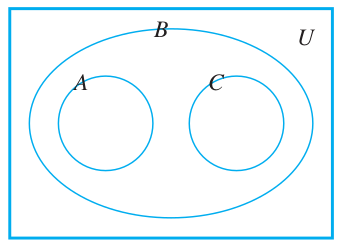
\includegraphics[scale=0.5]{../images/6.1.14.a.png}
\end{figure}
\end{proof}

\subsubsection{(b)}
\(C \subseteq A, B \cap C = \es\)

\begin{proof}
\begin{figure}[ht!]
\centering
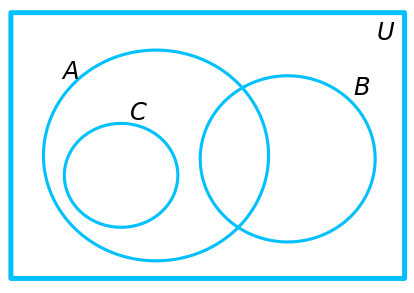
\includegraphics[scale=0.4]{../images/6.1.14.b.png}
\end{figure}
\end{proof}

\subsection{Exercise 15}
In each of the following, draw a Venn diagram for sets $A, B$, and $C$ that satisfy the given conditions.

\subsubsection{(a)}
\(A \cap B = \es, A \subseteq C, C \cap B \neq \es\)

\begin{proof}
\begin{figure}[ht!]
\centering
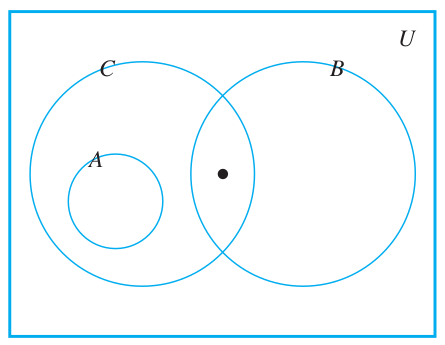
\includegraphics[scale=0.4]{../images/6.1.15.a.png}
\end{figure}
\end{proof}

\subsubsection{(b)}
\(A \subseteq B, C \subseteq B, A \cap C \neq \es\)

\begin{proof}
\begin{figure}[ht!]
\centering
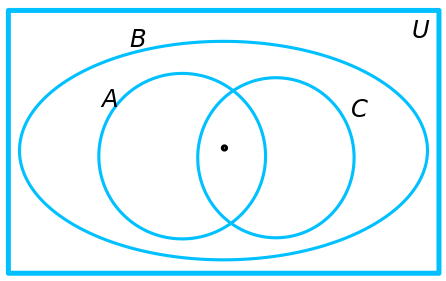
\includegraphics[scale=0.4]{../images/6.1.15.b.png}
\end{figure}
\end{proof}

\subsubsection{(c)}
\(A \cap B \neq \es, B \cap C \neq \es, A \cap C = \es, A \nsubseteq B, C \nsubseteq B\)

\begin{proof}
\begin{figure}[ht!]
\centering
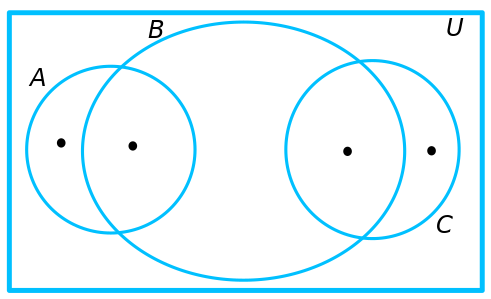
\includegraphics[scale=0.4]{../images/6.1.15.c.png}
\end{figure}
\end{proof}

\subsection{Exercise 16}
Let \(A = \{a, b, c\}, B = \{b, c, d\}, C = \{b, c, e\}\).

\subsubsection{(a)}
Find \(A \cup (B \cap C), (A \cup B) \cap C\), and \((A \cup B) \cap (A \cup C)\). Which of these sets are equal?

\begin{proof}
\(A \cup (B \cap C ) = \{a, b, c\}, (A \cup B) \cap C =
\{b, c\}\), 
and \((A \cup B) \cap (A \cup C ) = \{a, b, c, d\} \cap \{a, b, c, e\} = \{a, b, c\}\). 
Hence \(A \cup (B \cap C ) = (A \cup B) \cap (A \cup C).\)
\end{proof}

\subsubsection{(b)}
Find \(A \cap (B \cup C), (A \cap B) \cap C\), and \((A \cap B) \cup (A \cap C)\). Which of these sets are equal?

\begin{proof}
\(A \cap (B \cup C ) = \{b, c\}, (A \cap B) \cap C =
\{b, c\}\), 
and \((A \cap B) \cup (A \cap C ) = \{b, c\} \cup \{b, c\} = \{b, c\}\). 
Hence all three sets are equal.
\end{proof}

\subsubsection{(c)}
Find \((A - B) - C\) and \(A - (B - C)\). Are these sets equal?

\begin{proof}
\((A - B) - C = \{a\} - \{b, c, e\} = \{a\}\) and \(A - (B - C) = \{a, b, c\} - \{d\} = \{a, b, c\}\).
The sets are not equal.
\end{proof}

\subsection{Exercise 17}
\begin{figure}[ht!]
\centering
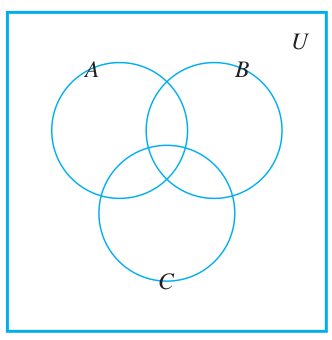
\includegraphics[scale=0.3]{../images/6.1.17.png}
\end{figure}
Consider the Venn diagram. For each of (a)-(f), copy the diagram and shade the region corresponding to the indicated set.

\subsubsection{(a)}
$A \cap B$

\begin{proof}
\begin{figure}[ht!]
\centering
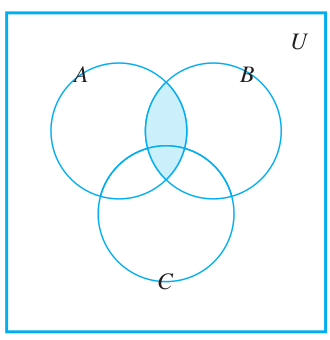
\includegraphics[scale=0.3]{../images/6.1.17.a.png}
\end{figure}
\end{proof}

\subsubsection{(b)}
$B \cup C$

\begin{proof}
\begin{figure}[ht!]
\centering
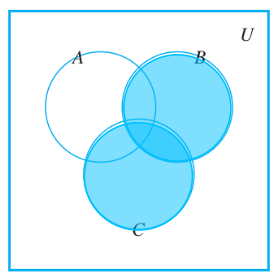
\includegraphics[scale=0.4]{../images/6.1.17.b.png}
\end{figure}
\end{proof}

\subsubsection{(c)}
$A^c$

\begin{proof}
\begin{figure}[ht!]
\centering
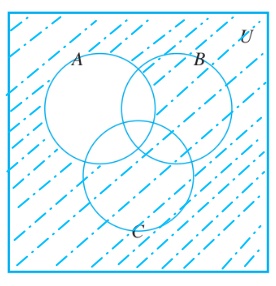
\includegraphics[scale=0.4]{../images/6.1.17.c.png}
\end{figure}
\end{proof}

\subsubsection{(d)}
$A - (B \cup C)$

\begin{proof}
\begin{figure}[ht!]
\centering
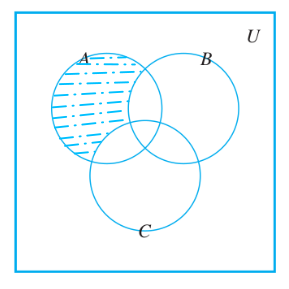
\includegraphics[scale=0.4]{../images/6.1.17.d.png}
\end{figure}
\end{proof}

\subsubsection{(e)}
$(A \cup B)^c$

\begin{proof}
\begin{figure}[ht!]
\centering
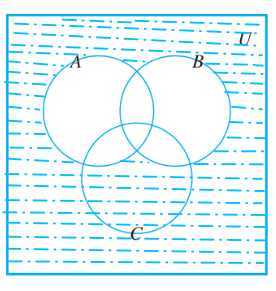
\includegraphics[scale=0.4]{../images/6.1.17.e.png}
\end{figure}
\end{proof}

\subsubsection{(f)}
$A^c \cap B^c$

\begin{proof}
Same as (e).
\end{proof}

\subsection{Exercise 18}

\subsubsection{(a)}
Is the number 0 in $\es$? Why?

\begin{proof}
The number 0 is not in $\es$ because $\es$ has no elements.
\end{proof}

\subsubsection{(b)}
Is $\es = \{\es\}$? Why?

\begin{proof}
No. The left-hand set is the empty set; it does not have any elements. The right-hand set is a set with one element, namely $\es$.
\end{proof}

\subsubsection{(c)}
Is $\es \in \{\es\}$? Why?

\begin{proof}
Yes. The left-hand side is the empty set; the right-hand side is a set with one element, namely $\es$. So the left-
hand side is an element of the right-hand side.
\end{proof}

\subsubsection{(d)}
Is $\es \in \es$? Why?

\begin{proof}
$\es$ is not in $\es$ because $\es$ has no elements.
\end{proof}

\subsection{Exercise 19}
Let \(A_i = \{i, i^2\}\) for each integer \(i = 1, 2, 3, 4\).

\subsubsection{(a)}
\(A_1 \cup A_2 \cup A_3 \cup A_4 = ?\)

\begin{proof}
\(A_1 = \{1, 1^2\} = \{1\}, A_2 = \{2, 2^2\} = \{2, 4\}, A_3 = \{3, 3^2\} = \{3, 9\}, A_4 = \{4, 4^2\} = \{4, 16\}\)

\(A_1 \cup A_2 \cup A_3 \cup A_4 = \{1\} \cup \{2, 4\} \cup \{3, 9\} \cup \{4, 16\} = \{1, 2, 3, 4, 9, 16\}\)
\end{proof}

\subsubsection{(b)}
\(A_1 \cap A_2 \cap A_3 \cap A_4 = ?\)

\begin{proof}
\(A_1 \cap A_2 \cap A_3 \cap A_4 = \{1\} \cap \{2, 4\} \cap \{3, 9\} \cap \{4, 16\} = \es\)
\end{proof}

\subsubsection{(c)}
Are \(A_1, A_2, A_3, A_4\) mutually disjoint? Explain.

\begin{proof}
\(A_1, A_2, A_3, A_4\) are not mutually disjoint, because \(A_2 \cap A_4 = \{4\} \neq \es\).
\end{proof}

\subsection{Exercise 20}
Let \(B_i = \{x \in \R \, | \, 0 \leq x \leq i\}\) for each integer \(i = 1, 2, 3, 4\).

\subsubsection{(a)}
\(B_1 \cup B_2 \cup B_3 \cup B_4 = ?\)

\begin{proof}
\(B_1 \cup B_2 \cup B_3 \cup B_4 = B_4 = [0, 4]\)
\end{proof}

\subsubsection{(b)}
\(B_1 \cap B_2 \cap B_3 \cap B_4 = ?\)

\begin{proof}
\(B_1 \cap B_2 \cap B_3 \cap B_4 = B_1 = [0, 1]\)
\end{proof}

\subsubsection{(c)}
Are \(B_1, B_2, B_3, B_4\) mutually disjoint? Explain.

\begin{proof}
No, because for example \(B_1 \cap B_2 = B_1 \neq \es\).
\end{proof}

\subsection{Exercise 21}
Let \(C_i = \{-i, i\}\) for each nonnegative integer $i$.

\subsubsection{(a)}
\(\dps \bigcup_{i=0}^{4}C_i = ?\)

\begin{proof}
\(C_0 = \{0, -0\} = \{0\}, C_1 = \{1, -1\}, C_2 = \{2, -2\}, C_3 = \{3, -3\}, C_4 = \{4, -4\}\)

\(\dps \bigcup_{i=0}^{4}C_i = \{-4, -3, -2, -1, 0, 1, 2, 3, 4\}\)
\end{proof}

\subsubsection{(b)}
\(\dps \bigcap_{i=0}^{4}C_i = ?\)

\begin{proof}
\(\dps \bigcap_{i=0}^{4}C_i = \{0\} \cap \{1, -1\} \cap \{2, -2\} \cap \{3, -3\} \cap \{4, -4\} = \es\)
\end{proof}

\subsubsection{(c)}
Are \(C_0, C_1, C_2, \ldots\) mutually disjoint? Explain.

\begin{proof}
$C_0, C_1, C_2, \ldots$ are mutually disjoint because no two of the sets have any elements in common.
\end{proof}

\subsubsection{(d)}
\(\dps \bigcup_{i=0}^{n}C_i = ?\)

\begin{proof}
\(\dps \bigcup_{i=0}^{n}C_i = \{-n, -(n-1), \ldots, -2, -1, 0, 1, 2, \ldots, n-1, n\}\)
\end{proof}

\subsubsection{(e)}
\(\dps \bigcap_{i=0}^{n}C_i = ?\)

\begin{proof}
\(\dps \bigcap_{i=0}^{n}C_i = \es\)
\end{proof}

\subsubsection{(f)}
\(\dps \bigcup_{i=0}^{\infty}C_i = ?\)

\begin{proof}
\(\dps \bigcup_{i=0}^{\infty}C_i = \Z\), the set of all integers
\end{proof}

\subsubsection{(g)}
\(\dps \bigcap_{i=0}^{\infty}C_i = ?\)

\begin{proof}
\(\dps \bigcap_{i=0}^{\infty}C_i = \es\)
\end{proof}

\subsection{Exercise 22}
Let \(D_i = \{x \in \R \,|\, -i \leq x \leq i\} = [-i, i]\) for each nonnegative integer $i$.

\subsubsection{(a)}
\(\dps \bigcup_{i=0}^{4}D_i = ?\)

\begin{proof}
\(D_0 = [-0, 0] = \{0\}, D_1 = [-1, 1], D_2 = [-2, 2], D_3 = [-3, 3], D_4 = [-4, 4]\)

\(\dps \bigcup_{i=0}^{4}D_i = \{0\} \cup [-1, 1] \cup [-2, 2] \cup [-3, 3] \cup [-4, 4] = [-4, 4]\)
\end{proof}

\subsubsection{(b)}
\(\dps \bigcap_{i=0}^{4}D_i = ?\)

\begin{proof}
\(\dps \bigcap_{i=0}^{4}D_i = \{0\} \cap [-1, 1] \cap [-2, 2] \cap [-3, 3] \cap [-4, 4] = \{0\}\)
\end{proof}

\subsubsection{(c)}
Are \(D_0, D_1, D_2, \ldots\) mutually disjoint? Explain.

\begin{proof}
$D_0, D_1, D_2, \ldots,$ are not mutually disjoint. In fact, each \(D_k \subseteq D_{k+1}\).
\end{proof}

\subsubsection{(d)}
\(\dps \bigcup_{i=0}^{n}D_i = ?\)

\begin{proof}
\(\dps \bigcup_{i=0}^{n}D_i = [-n, n]\)
\end{proof}

\subsubsection{(e)}
\(\dps \bigcap_{i=0}^{n}D_i = ?\)

\begin{proof}
\(\dps \bigcap_{i=0}^{n}D_i = \{0\}\)
\end{proof}

\subsubsection{(f)}
\(\dps \bigcup_{i=0}^{\infty}D_i = ?\)

\begin{proof}
\(\dps \bigcup_{i=0}^{\infty}D_i = \R\), the set of all real numbers
\end{proof}

\subsubsection{(g)}
\(\dps \bigcap_{i=0}^{\infty}D_i = ?\)

\begin{proof}
\(\dps \bigcap_{i=0}^{\infty}D_i = \{0\}\)
\end{proof}

\subsection{Exercise 23}
Let \(V_i = \{x \in \R \,|\, -\frac{1}{i} \leq x \leq \frac{1}{i}\} = [-\frac{1}{i}, \frac{1}{i}]\) 
for each positive integer $i$.

\subsubsection{(a)}
\(\dps \bigcup_{i=1}^{4}V_i = ?\)

\begin{proof}
\(\dps \bigcup_{i=1}^{4}V_i = V_1 = [-1, 1]\)
\end{proof}

\subsubsection{(b)}
\(\dps \bigcap_{i=1}^{4}V_i = ?\)

\begin{proof}
\(\dps \bigcap_{i=1}^{4}V_i = V_4 = \left[-\frac{1}{4}, \frac{1}{4}\right]\)
\end{proof}

\subsubsection{(c)}
Are \(V_1, V_2, V_3, \ldots\) mutually disjoint? Explain.

\begin{proof}
$V_1, V_2, V_3, \ldots,$ are not mutually disjoint. In fact, each \(V_{k+1} \subseteq V_k\).
\end{proof}

\subsubsection{(d)}
\(\dps \bigcup_{i=1}^{n}V_i = ?\)

\begin{proof}
\(\dps \bigcup_{i=1}^{n}V_i = V_1 = [-1, 1]\)
\end{proof}

\subsubsection{(e)}
\(\dps \bigcap_{i=1}^{n}V_i = ?\)

\begin{proof}
\(\dps \bigcap_{i=1}^{n}V_i = V_n = \left[-\frac{1}{n}, \frac{1}{n}\right]\)
\end{proof}

\subsubsection{(f)}
\(\dps \bigcup_{i=1}^{\infty}V_i = ?\)

\begin{proof}
\(\dps \bigcup_{i=1}^{\infty}V_i = V_1 = [-1, 1]\)
\end{proof}

\subsubsection{(g)}
\(\dps \bigcap_{i=1}^{\infty}V_i = ?\)

\begin{proof}
\(\dps \bigcap_{i=1}^{\infty}V_i = \{0\}\)
\end{proof}

\subsection{Exercise 24}
Let \(W_i = \{x \in \R \,|\, i < x\} = (i, \infty)\) for each nonnegative integer $i$.

\subsubsection{(a)}
\(\dps \bigcup_{i=0}^{4}W_i = ?\)

\begin{proof}
\(\dps \bigcup_{i=0}^{4}W_i = W_0 = (0, \infty)\)
\end{proof}

\subsubsection{(b)}
\(\dps \bigcap_{i=0}^{4}W_i = ?\)

\begin{proof}
\(\dps \bigcap_{i=0}^{4}W_i = W_4 = (4, \infty)\)
\end{proof}

\subsubsection{(c)}
Are \(W_0, W_1, W_2, \ldots\) mutually disjoint? Explain.

\begin{proof}
$W_0, W_1, W_2, \ldots,$ are not mutually disjoint. In fact, each \(W_{k+1} \subseteq W_k\).
\end{proof}

\subsubsection{(d)}
\(\dps \bigcup_{i=0}^{n}W_i = ?\)

\begin{proof}
\(\dps \bigcup_{i=0}^{n}W_i = W_0 = (0, \infty)\)
\end{proof}

\subsubsection{(e)}
\(\dps \bigcap_{i=0}^{n}W_i = ?\)

\begin{proof}
\(\dps \bigcap_{i=0}^{n}W_i = W_n = (n, \infty)\)
\end{proof}

\subsubsection{(f)}
\(\dps \bigcup_{i=0}^{\infty}W_i = ?\)

\begin{proof}
\(\dps \bigcup_{i=0}^{\infty}W_i = W_0 = (0, \infty)\)
\end{proof}

\subsubsection{(g)}
\(\dps \bigcap_{i=0}^{\infty}W_i = ?\)

\begin{proof}
\(\dps \bigcap_{i=0}^{\infty}W_i = \es\)
\end{proof}

\subsection{Exercise 25}
Let \(R_i = \{x \in \R \,|\, 1 \leq x \leq 1 + \frac{1}{i}\} = \left[1, 1 + \frac{1}{i}\right]\) 
for each positive integer $i$.

\subsubsection{(a)}
\(\dps \bigcup_{i=1}^{4}R_i = ?\)

\begin{proof}
\(\dps \bigcup_{i=1}^{4}R_i = R_1 = [1, 2]\)
\end{proof}

\subsubsection{(b)}
\(\dps \bigcap_{i=1}^{4}R_i = ?\)

\begin{proof}
\(\dps \bigcap_{i=1}^{4}R_i = R_4 = \left[1, \frac{5}{4}\right]\)
\end{proof}

\subsubsection{(c)}
Are \(R_1, R_2, R_3, \ldots\) mutually disjoint? Explain.

\begin{proof}
No, in fact each \(R_{k+1} \subseteq R_k\).
\end{proof}

\subsubsection{(d)}
\(\dps \bigcup_{i=1}^{n}R_i = ?\)

\begin{proof}
\(\dps \bigcup_{i=1}^{n}R_i = R_1 = [1, 2]\)
\end{proof}

\subsubsection{(e)}
\(\dps \bigcap_{i=1}^{n}R_i = ?\)

\begin{proof}
\(\dps \bigcap_{i=1}^{n}R_i = R_n = \left[1, 1+\frac{1}{n}\right]\)
\end{proof}

\subsubsection{(f)}
\(\dps \bigcup_{i=1}^{\infty}R_i = ?\)

\begin{proof}
\(\dps \bigcup_{i=1}^{\infty}R_i = R_1 = [1, 2]\)
\end{proof}

\subsubsection{(g)}
\(\dps \bigcap_{i=1}^{\infty}R_i = ?\)

\begin{proof}
\(\dps \bigcap_{i=1}^{\infty}R_i = \{1\}\)
\end{proof}

\subsection{Exercise 26}
Let \(S_i = \{x \in \R \,|\, 1 < x < 1 + \frac{1}{i}\} = \left(1, 1 + \frac{1}{i}\right)\) 
for each positive integer $i$.

\subsubsection{(a)}
\(\dps \bigcup_{i=1}^{4}S_i = ?\)

\begin{proof}
\(\dps \bigcup_{i=1}^{4}S_i = S_1 = (1, 2)\)
\end{proof}

\subsubsection{(b)}
\(\dps \bigcap_{i=1}^{4}S_i = ?\)

\begin{proof}
\(\dps \bigcap_{i=1}^{4}S_i = S_4 = (1, 5/4)\)
\end{proof}

\subsubsection{(c)}
Are \(S_0, S_1, S_2, \ldots\) mutually disjoint? Explain.

\begin{proof}
No, in fact each \(S_{k+1} \subseteq S_k\).
\end{proof}

\subsubsection{(d)}
\(\dps \bigcup_{i=1}^{n}S_i = ?\)

\begin{proof}
\(\dps \bigcup_{i=1}^{n}S_i = S_1 = (1, 2)\)
\end{proof}

\subsubsection{(e)}
\(\dps \bigcap_{i=1}^{n}S_i = ?\)

\begin{proof}
\(\dps \bigcap_{i=1}^{n}S_i = S_n = (1, \frac{n+1}{n})\)
\end{proof}

\subsubsection{(f)}
\(\dps \bigcup_{i=1}^{\infty}S_i = ?\)

\begin{proof}
\(\dps \bigcup_{i=1}^{\infty}S_i = S_1 = (1, 2)\)
\end{proof}

\subsubsection{(g)}
\(\dps \bigcap_{i=1}^{\infty}S_i = ?\)

\begin{proof}
\(\dps \bigcap_{i=1}^{\infty}S_i = (1, 1) = \es\)
\end{proof}

\subsection{Exercise 27}

\subsubsection{(a)}
Is \(\{\{a, d, e\}, \{b, c\}, \{d, f\}\}\) a partition of
\(\{a, b, c, d, e, f\}\)?

\begin{proof}
No. The element $d$ is in two of the sets.
\end{proof}

\subsubsection{(b)}
Is \(\{\{w, x, v\}, \{u, y, q\}, \{p, z\}\}\) a partition of \(\{p, q, u, v, w, x, y, z\}\)?

\begin{proof}
Yes.
\end{proof}

\subsubsection{(c)}
Is \(\{\{5, 4\}, \{7, 2\}, \{1, 3, 4\}, \{6, 8\}\}\) a partition of \(\{1, 2, 3, 4, 5, 6, 7, 8\}\)?

\begin{proof}
No. The element $4$ is in two of the sets.
\end{proof}

\subsubsection{(d)}
Is \(\{\{3, 7, 8\}, \{2, 9\}, \{1, 4, 5\}\}\) a partition of \(\{1, 2, 3, 4, 5, 6, 7, 8, 9\}\)?

\begin{proof}
No. None of the sets contains 6.
\end{proof}

\subsubsection{(e)}
Is \(\{\{1, 5\}, \{4, 7\}, \{2, 8, 6, 3\}\}\) a partition of \(\{1, 2, 3, 4, 5, 6, 7, 8\}\)?

\begin{proof}
Yes.
\end{proof}

\subsection{Exercise 28}
Let $E$ be the set of all even integers and $O$ the set of all odd integers. Is \(\{E, O\}\) a partition of $\Z$, the set of all integers? Explain your answer.

\begin{proof}
Yes. Every integer is either even or odd, and no integer is both even and odd.
\end{proof}

\subsection{Exercise 29}
Let $\R$ be the set of all real numbers. Is $\{R^+, R^-, \{0\}\}$ a partition of $\R$? Explain your answer.

\begin{proof}
Yes. Every real number is either positive or negative or zero, and no real number is both positive and negative, and 
zero is neither negative nor positive (so the three sets are mutually disjoint).
\end{proof}

\subsection{Exercise 30}
Let $Z$ be the set of all integers and let
\begin{center}
\begin{tabular}{rcl}
$A_1$ & = & \(\{n \in \Z \, | \, n = 4k \text{ for some integer } k\}\) \\
$A_2$ & = & \(\{n \in \Z \, | \, n = 4k + 1 \text{ for some integer } k\}\) \\
$A_3$ & = & \(\{n \in \Z \, | \, n = 4k + 2 \text{ for some integer } k\}\) \\
$A_4$ & = & \(\{n \in \Z \, | \, n = 4k + 3 \text{ for some integer } k\}\) 
\end{tabular}
\end{center}
Is \(\{A_0, A_1, A_2, A_3\}\) a partition of $\Z$? Explain your answer.

\begin{proof}
Yes. These sets are mutually disjoint, and by the quotient-remainder theorem, every integer has exactly one of the 
forms \(n = 4k\) or \(n = 4k+1\) or \(n = 4k+2\) or \(n = 4k+3\).
\end{proof}

\subsection{Exercise 31}
Suppose \(A = \{1, 2\}, B = \{2, 3\}\). Find each of the following:

\subsubsection{(a)}
\(\ps(A \cap B)\)

\begin{proof}
\(A \cap B = \{2\}\), so \(\ps(A \cap B) = \{\es, \{2\}\}\).
\end{proof}

\subsubsection{(b)}
\(\ps(A)\)

\begin{proof}
\(A = \{1, 2\}\), so \(\ps(A) = \{\es, \{1\}, \{2\}, \{1, 2\}\}\).
\end{proof}

\subsubsection{(c)}
\(\ps(A \cup B)\)

\begin{proof}
\(A \cup B = \{1, 2, 3\}\), so \(\ps(A \cup B) = \{\es, \{1\}, \{2\}, \{3\}, \{1, 2\}, \{1, 3\}, \{2, 3\}, \{1, 2, 3\}\}\).
\end{proof}

\subsubsection{(d)}
\(\ps(A \times B)\)

\begin{proof}
\(A \times B = \{(1, 2), (1, 3), (2, 2), (2, 3)\}\), so \(\ps(A\times B)=\{\es, \{(1, 2)\},\{(1, 3)\},\{(2, 2)\},\)

\(\{(2, 3)\}, \{(1, 2), (1, 3)\}, \{(1, 2), (2, 2)\}, \{(1, 2), (2, 3)\}, \{(1, 3), (2, 2)\}, \{(1, 3), (2, 3)\}, \)

\(\{(2, 2), (2, 3)\}, \{(1, 2), (1, 3), (2, 2)\}, \{(1, 2), (1, 3), (2, 3)\}, \{(1, 2), (2, 2), (2, 3)\}, \)

\(\{(1, 3), (2, 2), (2, 3)\}, \{(1, 2), (1, 3), (2, 2), (2, 3)\}\}\).
\end{proof}

\subsection{Exercise 32}

\subsubsection{(a)}
Suppose \(A = \{1\}, B = \{u, v\}\). Find \(\ps(A \times B)\).

\begin{proof}
\(\ps(A \times B) = \{\es, \{(1, u)\}, \{(1, v)\}, \{(1, u), (1, v)\}\}\)
\end{proof}

\subsubsection{(b)}
Suppose \(X = \{a, b\}, Y = \{x, y\}\). Find \(\ps(X \times Y)\).

\begin{proof}
\(X \times Y = \{(a, x), (a, y), (b, x), (b, y)\}\)

\(\ps(X \times Y) = \{\es, \{(a, x)\}, \{(a, y)\}, \{(b, x)\}, \{(b, y)\}, \{(a, x), (a, y)\}, \{(a, x), (b, x)\},\)

\(\{(a, x), (b, y)\}, \{(a, y), (b, x)\}, \{(a, y), (b, y)\}, \{(b, x), (b, y)\}, \{(a, x), (a, y), (b, x)\},\) 

\(\{(a, x), (a, y), (b, y)\}, \{(a, x), (b, x), (b, y)\}, \{(a, y), (b, x), (b, y)\},\) 

\(\{(a, x), (a, y), (b, x), (b, y)\}\}\)
\end{proof}

\subsection{Exercise 33}

\subsubsection{(a)}
Find \(\ps(\es)\).

\begin{proof}
\(\ps(\es) = \{\es\}\)
\end{proof}

\subsubsection{(b)}
Find \(\ps(\ps(\es))\).

\begin{proof}
\(\ps(\ps(\es)) = \ps(\{\es\}) = \{\es, \{\es\}\}\)
\end{proof}

\subsubsection{(c)}
Find \(\ps(\ps(\ps(\es)))\).

\begin{proof}
\(\ps(\ps(\ps(\es))) = \ps(\{\es, \{\es\}\}) = \{\es, \{\es\}, \{\{\es\}\}, \{\es, \{\es\}\}\}\)
\end{proof}

\subsection{Exercise 34}
Let \(A_1 = \{1\}, A_2 = \{u, v\}, A_3 = \{m, n\}\). Find each of the following sets:

\subsubsection{(a)}
$A_1 \cup (A_2 \times A_3)$

\begin{proof}
\(A_1 \cup (A_2 \times A_3) = \{1\} \cup \{(u, m), (u, n), (v, m), (v, n)\}\)

\(= \{1, (u, m), (u, n), (v, m), (v, n)\}\)
\end{proof}

\subsubsection{(b)}
$(A_1 \cup A_2) \times A_3$

\begin{proof}
\((A_1 \cup A_2) \times A_3 = \{1, u, v\} \times \{m, n\} = \{(1, m), (1, n), (u, m), (u, n), (v, m), (v, n)\}\)
\end{proof}

\subsection{Exercise 35}
Let \(A = \{a, b\}, B = \{1, 2\}, C = \{2, 3\}\). Find each of the following sets.

\subsubsection{(a)}
$A \times (B \cup C)$

\begin{proof}
\(A \times (B \cup C) = \{a, b\} \times \{1, 2, 3\}\ = \{(a, 1), (a, 2), (a, 3), (b, 1), (b, 2), (b, 3)\}\)
\end{proof}

\subsubsection{(b)}
$(A \times B) \cup (A \times C)$

\begin{proof}
\((A \times B) \cup (A \times C) = \{(a, 1), (a, 2), (b, 1), (b, 2), (a, 2), (a, 3), (b, 2), (b, 3)\}\) 

\(= \{(a, 1), (a, 2), (b, 1), (b, 2), (a, 3), (b, 3)\}\)
\end{proof}

\subsubsection{(c)}
$A \times (B \cap C)$

\begin{proof}
\(A \times (B \cap C) = \{a, b\} \times \{2\}\ = \{(a, 2), (b, 2)\}\)
\end{proof}

\subsubsection{(d)}
$(A \times B) \cap (A \times C)$

\begin{proof}
\((A \times B) \cap (A \times C) = \{(a, 1), (a, 2), (b, 1), (b, 2)\} \cap \{(a, 2), (a, 3), (b, 2), (b, 3)\}\) 

\(= \{(a, 2), (b, 2)\}\)
\end{proof}

\subsection{Exercise 36}
Trace the action of Algorithm 6.1.1 on the variables $i, j, found$, and $answer$ for $m = 3, n = 3$, and sets $A$ and 
$B$ represented as the arrays \(a[1] = u, a[2] = v, a[3] = w, b[1] = w, b[2] = u, b[3] = v\).

\begin{proof}
\begin{figure}[ht!]
\centering
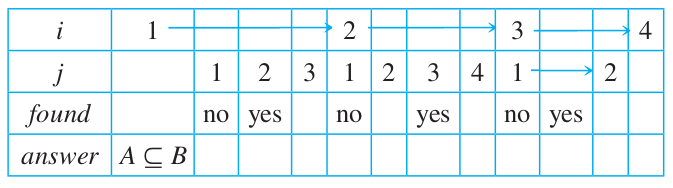
\includegraphics[scale=0.5]{../images/6.1.36.png}
\end{figure}
\end{proof}

\subsection{Exercise 37}
Trace the action of Algorithm 6.1.1 on the variables $i, j, found$, and $answer$ for $m = 4, n = 4$, and sets $A$ and 
$B$ represented as the arrays \(a[1] = u, a[2] = v, a[3] = w, a[4] = x, b[1] = r, b[2] = u, b[3] = y, b[4] = z\).

\begin{proof}
\begin{center}
\arrayrulecolor{cyan} % change rule color
\begin{tabular}{|l|c|c|c|c|c|c|c|c|}
\hline
{\bf i} & 1 & & & & 2 & & & \\
\hline
{\bf j} & 1 & 2 & 3 & 4 & 1 & 2 & 3 & 4 \\
\hline
{\bf found} & no & yes & & & no & & & \\
\hline
{\bf answer} & \(A \subseteq B\) & & & & & & & \(A \nsubseteq B\) \\
\hline
\end{tabular}
\arrayrulecolor{black} % change it back!
\end{center}
\end{proof}

\subsection{Exercise 38}
Write an algorithm to determine whether a given element $x$ belongs to a given set that is represented as the array 
\(a[1], a[2], \ldots, a[n]\).

\begin{tcolorbox}[colframe=cyan]
{\bf \cy Algorithm: Testing whether $x \in A$} 

{\bf \cy Input:} $x$ (an element), $n$ (a positive integer), \(a[1], \ldots, a[n]\) (a one-dimensional array 
representing the set $A$).

{\bf \cy Algorithm Body:}
\begin{tabbing}
\(i \coloneqq 1, answer \coloneqq\) ``\(x \notin A\)'' \\
{\bf while} \= (\(i \leq n\) and \(answer =\) ``\(x \notin A\)'') \\
            \> {\bf if} \(x = a[i]\) {\bf then} \(answer = \) ``\(x \in A\)'' \\
            \> \(i \coloneqq i + 1\) \\
{\bf end while}
\end{tabbing}
{\bf \cy Output:} {\it answer [a string]}
\end{tcolorbox}

\section{Exercise Set 6.2}
{\bf \cy Fill the blanks.}

\subsection{Exercise 1}
\subsubsection{(a)}
To say that an element is in \(A \cap (B \cup C)\) means that it is in (1) \fbl and in (2) \fbl.

\begin{proof}
(1) $A$ (2) \(B \cup C\)

\end{proof}

\subsubsection{(b)}
To say that an element is in \((A \cap B) \cup C\) means that it is in (1) \fbl or in (2) \fbl.

\begin{proof}
(1) \(A \cap B\) (2) $C$
\end{proof}

\subsubsection{(c)}
To say that an element is in \(A - (B \cap C)\) means that it is in (1) \fbl and not in (2) \fbl.

\begin{proof}
(1) $A$ (2) \(B \cap C\)
\end{proof}

\subsubsection{(d)}
To prove that \((A \cup B) \cap C \subseteq A \cup (B \cap C)\), we suppose that $x$ is any element in (1) \fbl. 
Then we must show that (2) \fbl.

\begin{proof}
(1) \((A \cup B) \cap C\) (2) \(A \cup (B \cap C)\)
\end{proof}

\subsubsection{(e)}
If $A, B$, and $C$ are any sets such that \(B \subseteq C\), to prove that \(A \cap B \subseteq A \cap C\), we 
suppose that $x$ is any element in (1) \fbl. Then we must show that (2) \fbl.

\begin{proof}
(1) \(A \cap B\) (2) \(A \cap C\)
\end{proof}

\subsection{Exercise 2}
The following are two proofs that for all sets $A$ and $B$, \(A - B \subseteq A\). The first is less formal, and the 
second is more formal. Fill in the blanks.

\subsubsection{(a)}
\underline{Proof:} Suppose $A$ and $B$ are any sets. To show that \(A - B \subseteq A\), we must show that every 
element in (1) \fbl is in (2) \fbl. But any element in \(A - B\) is in (3) \fbl and not in (4) \fbl (by definition of 
\(A - B\)). In particular, such an element is in $A$.

\begin{proof}
(1) $A - B$ (2) $A$ (3) $A$ (4) $B$
\end{proof}

\subsubsection{(b)}
\underline{Proof:} Suppose $A$ and $B$ are any sets and \(x \in A - B\). {\it [We must show that (1) \fbl.]} By 
definition of set difference, \(x \in (2)\) \fbl and \(x \notin (3)\) \fbl. In particular, \(x \in (4)\) 
{\it [which is what was to be shown].}

\begin{proof}
(1) $x \in A$ (2) $A$ (3) $B$ (4) $A$
\end{proof}

{\bf \cy In 3 and 4, supply explanations of the steps in the given proofs.}

\subsection{Exercise 3}
\underline{Theorem:} For all sets $A, B$, and $C$, if \(A \subseteq B\) and \(B \subseteq C\) then \(A \subseteq C\).

\underline{Proof:}
\begin{center}
\arrayrulecolor{cyan} % change rule color
\begin{tabular}{|l|l|}
\hline
{\bf Statement} & {\bf Explanation} \\ 
\hline
Suppose $A, B, C$ are any sets such that & starting point \\
\(A \subseteq B\) and \(B \subseteq C\). & \\
\hline
We must show that \(A \subseteq C\). & conclusion to be shown \\
\hline
Let $x$ be any element in $A$. & start of an element proof \\
\hline
Then $x$ is in $B$. & {\cy (a)} \fbl \\
\hline
It follows that $x$ is in $C$. & {\cy (b)} \fbl \\
\hline
Thus every element of $A$ is in $C$. & since $x$ could be any element of $A$ \\
\hline
Therefore \(A \subseteq C\) {\it [as was to be shown].} & {\cy (c)} \fbl \\
\hline
\end{tabular}
\arrayrulecolor{black} % change it back!
\end{center}

\begin{proof}
(a) by definition of subset (because $A \subseteq B$) (b) by definition of subset (because $B \subseteq C$) 
(c) by definition of subset
\end{proof}

\subsection{Exercise 4}
\underline{Theorem:} For all sets $A, B$, if \(A \subseteq B\) then \(A \cup B \subseteq B\).

\underline{Proof:}
\begin{center}
\arrayrulecolor{cyan} % change rule color
\begin{tabular}{|l|l|}
\hline
{\bf Statement} & {\bf Explanation} \\ 
\hline
Suppose $A, B$ are any sets such that \(A \subseteq B\). & starting point \\
\hline
We must show that \(A \cup B \subseteq B\). & conclusion to be shown \\
\hline
Let $x$ be any element in $A \cup B$. & start of an element proof \\
\hline
Then $x \in A$ or $x \in B$. & {\cy (a)} \fbl \\
\hline
In case $x \in A$, then $x \in B$. & {\cy (b)} \fbl \\
\hline
In case $x \in B$, then $x \in B$. & tautology ($p \to p)$ \\
\hline
So in either case $x \in B$. & proof by division into cases \\
\hline
Thus every element of $A \cup B$ is in $B$. & since $x$ could be any element of $A \cup B$ \\
\hline
Therefore \(A \cup B \subseteq B\) {\it [as was to be shown].} & {\cy (c)} \fbl \\
\hline
\end{tabular}
\arrayrulecolor{black} % change it back!
\end{center}

\begin{proof}
(a) by definition of union (b) by definition of subset (because \(A \subseteq B\)) (c) by definition of subset
\end{proof}

\subsection{Exercise 5}
Prove that for all sets $A$ and $B$, \((B - A) = B \cap A^c\).

\begin{proof}
Suppose $A$ and $B$ are any sets.

{\bf Proof that \(B - A \subseteq B \cap A^c\):} Suppose \(x \in B - A\). By definition of set difference, 
\(x \in B\) and \(x \notin A\). It follows by definition of complement that \(x \in B\) and \(x \in A^c\), and so by 
definition of intersection, \(x \in B \cap A^c\). {\it [Thus \(B - A \subseteq B \cap A^c\) by definition of subset.]}

{\bf Proof that \(B \cap A^c \subseteq B - A\):} Suppose \(x \in B \cap A^c\). By definition of intersection, 
\(x \in B\) and \(x \in A^c\). It follows by definition of complement that \(x \in B\) and \(x \notin A\), and so by 
definition of set difference, \(x \in B - A\). {\it [Thus \(B \cap A^c \subseteq B - A\) by definition of subset.]}

{\it [Since both subset relations have been proved, \(B - A = B \in A^c\) by definition of set equality.]}
\end{proof}

\subsection{Exercise 6}
Let $\cap$ and $\cup$ stand for the words “intersection” and “union,” respectively. Fill in the blanks in the 
following proof that for all sets $A, B$, and $C$, \(A \cap (B \cup C) = (A \cap B) \cup (A \cap C)\).

\underline{Proof:} Suppose $A$, $B$, and $C$ are any sets.

{\bf (1) Proof that \(A \cap (B \cup C) \subseteq (A \cap B) \cup (A \cap C)\):}

Let \(x \in A \cap (B \cup C)\). {\it [We must show that \(x \in {\cy (a) \fbl}\)].}

By definition of $\cup$, \(x \in {\cy (b) \fbl}\) and \(x \in B \cup C\). 
Thus \(x \in A\) and, by definition of $\cup$, \(x \in B\) or {\cy (c) \fbl}.

{\bf Case 1 (\(x \in A\) and \(x \in B\)):} In this case, \(x \in A \cap B\) by definition of $\cap$.

{\bf Case 2 (\(x \in A\) and \(x \in C\)):} In this case, \(x \in A \cap C\) by definition of $\cap$.

By cases 1 and 2, \(x \in A \cap B\) or \(x \in A \cap C\), and so, by definition of $\cup$, {\cy (d) \fbl}.

{\it [So \(A \cap (B \cup C ) \subseteq (A \cap B) \cup (A \cap C)\) by definition of subset.]}

{\bf (2) Proof that \((A \cap B) \cup (A \cap C) \subseteq A \cap (B \cup C)\):}

Let \(x \in (A \cap B) \cup (A \cap C)\). {\it [We must show that \(x \in A \cap (B \cup C )\).]}

By definition of $\cup$, \(x \in A \cap B\) {\cy (a) \fbl} \(x \in A \cap C.\)

{\bf Case 1 (\(x \in A \cap B\)):} In this case, by definition of $\cap$, \(x \in A\) and \(x \in B\). Since 
\(x \in B\), then \(x \in B \cup C\) by definition of $\cup$.

{\bf Case 2 (\(x \in A \cap C\)):} In this case, by definition of $\cap$, \(x \in A\) {\cy (b) \fbl} 
\(x \in C\). Since \(x \in C\), then \(x \in B \cup C\) by definition of $\cup$.

In both cases \(x \in A\) and \(x \in B \cup C\), and so, by definition of $\cap$, {\cy (c) \fbl}.

{\it [So \((A \cap B) \cup (A \cap C) \subseteq A \cap (B \cup C)\) by definition of {\cy (d) \fbl}.]}

{\bf (3) Conclusion:} {\it [Since both subset relations have been proved, it follows, by definition of set equality, that {\cy (a) \fbl}.]}

\begin{proof}
(1) (a) \((A \cap B) \cup (A \cap C)\) (b) $A$ (c) \(x \in C\) (d) \(x \in (A \cap B) \cup (A \cap C)\)

(2) (a) or (b) and (c) \(x \in A \cap (B \cup C)\) (d) subset

(3) (a) for all sets $A, B$, and $C$, \(A \cap (B \cup C) = (A \cap B) \cup (A \cap C)\).
\end{proof}

{\bf \cy Use an element argument to prove each statement in $7-22$. Assume that all sets are subsets of a universal set $U$.}

\subsection{Exercise 7}
For all sets $A$ and $B$, \((A \cap B)^c = A^c \cup B^c\).

\begin{proof}
Suppose $A$ and $B$ are any sets.

{\bf Proof that \((A \cap B)^c \subseteq A^c \cup B^c\):} Suppose \(x \in (A \cap B)^c\). By definition of 
complement, \(x \notin (A \cap B)\). It follows by definition of intersection that \(x \notin A\) or 
\(x \notin B\), and so by definition of complement, \(x \in A^c \) or \(x \in B^c\). So by definition of union, 
\(x \in A^c \cup B^c\). {\it [Thus \((A \cap B)^c \subseteq A^c \cup B^c\) by definition of subset.]}

{\bf Proof that \(A^c \cup B^c \subseteq (A \cap B)^c\):} Suppose \(x \in A^c \cup B^c\). By definition of union, 
\(x \in A^c\) or \(x \in B^c\). By definition of complement, \(x \notin A\) or \(x \notin B\). It follows by 
definition of intersection that \(x \notin (A \cap B)\). Then by definition of complement, \(x \in (A \cap B)^C\).
{\it [Thus \(A^c \cup B^c \subseteq (A \cap B)^c\) by definition of subset.]}

{\it [Since both subset relations have been proved, \((A \cap B)^c = A^c \cup B^c\) by definition of set equality.]}
\end{proof}

\subsection{Exercise 8}
For all sets $A$ and $B$, \((A \cap B) \cup (A \cap B^c) = A\). (This property is used in Section 9.9.)

\begin{proof}
Suppose $A$ and $B$ are any sets.

{\bf Proof that \((A \cap B) \cup (A \cap B^c) \subseteq A\):} Suppose \(x \in (A \cap B) \cup (A \cap B^c)\). 
{\it [We must show that \(x \in A\).]}

By definition of union, \(x \in A \cap B\) or \(x \in (A \cap B^c)\).

{\bf Case 1 \((x \in A \cap B)\):} In this case $x$ is in $A$ and $x$ is in $B$, and so, in particular, \(x \in A\).

{\bf Case 2 \((x \in A \cap B^c)\):} In this case $x$ is in $A$ and $x$ is not in $B$, and so, in particular, \(x \in A\).

Thus, in either case, \(x \in A\) {\it [as was to be shown].} 

So \((A \cap B) \cup (A \cap B c ) \subseteq A\) {\it [by definition of subset].}

{\bf Proof that \(A \subseteq (A \cap B) \cup (A \cap B^c )\):} Suppose \(x \in A\). {\it [We must show that 
\(x \in (A \cap B) \cup (A \cap B^c)\).]}

Either \(x \in B\) or \(x \notin B\).

{\bf Case 1 \((x \in B)\):} In this case we know that $x$ is in $A$ and we are also assuming that $x$ is in $B$. 
Hence, by definition of intersection, \(x \in A \cap B\).

{\bf Case 2 \((x \in A \cap B^c)\):} In this case we know that $x$ is in $A$ and we are also assuming that $x$ is in 
$B^c$. Hence, by definition of intersection, \(x \in A \cap B^c\).

Thus, in either case \(x \in A \cap B\) or \(x \in A \cap B^c\), and so, by definition of union, \(x \in (A \cap B) 
\cup (A \cap B^c)\) {\it [as was to be shown].} 

So \(A \subseteq (A \cap B) \cup (A \cap B^c)\) {\it [by definition of subset].}

{\bf Conclusion:} Since both subset relations have been proved it follows by definition of set equality that 
\((A \cap B) \cup (A \cap B^c) = A\).
\end{proof}

\subsection{Exercise 9}
For all sets $A$, $B$, and $C$, \((A - B) \cup (C - B) = (A \cup C) - B\).

\begin{proof}
Suppose $A$, $B$, and $C$ are any sets. 

To show that \((A - B) \cup (C - B) = (A \cup C ) - B\), we must show that \((A - B) \cup (C - B) \subseteq (A \cup C) - B\) 
and that \((A \cup C) - B \subseteq (A - B) \cup (C - B)\).

{\bf Proof that \((A - B) \cup (C - B) \subseteq (A \cup C) - B\):}

Suppose that $x$ is any element in \((A - B) \cup (C - B)\). {\it [We must show that \(x \in (A \cup C ) - B\).]} 
By definition of union, \(x \in A - B\) or \(x \in C - B\).

{\bf Case 1 (\(x \in A - B\)):} Then, by definition of set difference, \(x \in A\) and \(x \notin B\). Now because 
\(x \in A\), we have that \(x \in A \cup C\) by definition of union. Hence \(x \in A \cup C\) and \(x \notin B\), and 
so, by definition of set difference, \(x \in (A \cup C ) - B\).

{\bf Case 2 (\(x \in C - B\)):} Then, by definition of set difference, \(x \in C\) and \(x \notin B\). Now because 
\(x \in C\), we have that \(x \in A \cup C\) by definition of union. Hence \(x \in A \cup C\) and \(x \notin B\), and 
so, by definition of set difference, \(x \in (A \cup C) - B\). Thus, in both cases, \(x \in (A \cup C ) - B\) 
{\it [as was to be shown].} 

So \((A - B) \cup (C - B) \subseteq (A \cup C ) - B\) {\it [by definition of subset].}

To complete the proof that \((A - B ) \cup (C - B) = (A \cup C) - B\), you must show that 
\((A \cup C) - B \subseteq (A - B) \cup (C - B)\).
\end{proof}

\subsection{Exercise 10}
For all sets $A$, $B$, and $C$, \((A \cup B) \cap C \subseteq A \cup (B \cap C)\).

\begin{proof}
Suppose A, B, and C are any sets. We will show that \((A \cup B) \cap C \subseteq A \cup (B \cap C)\).

Suppose $x$ is any element \((A \cup B) \cap C\). By definition of intersection $x$ is in \(A \cup B\) and $x$ 
is in $C$. Then by definition of union $x$ is in $A$ or $x$ is in $B$, and in both cases $x$ is in $C$. It follows by 
definition of union that in case $x$ is in $A$ and $x$ is in $C$, then $x$ is in \(A \cup (B \cap C)\) by virtue of 
being in $A$. And in case $x$ is in \(B \cap C\), then $x$ is in \(A \cup (B \cap C)\) by virtue of being in 
\(B \cap C\). Thus in both cases $x$ is in \(A \cup (B \cap C )\), which proves that every element in \((A \cup B) \cap C\)
is in \(A \cup (B \cap C)\). Hence \((A \cup B) \cap C \subseteq A \cup (B \cap C)\) by definition of subset.
\end{proof}

\subsection{Exercise 11}
For all sets $A$, $B$, and $C$, \(A \cap (B - C) \subseteq (A \cap B) - (A \cap C)\).

\begin{proof}
Assume $A,B,C$ are any sets.

1. Assume \(x \in A \cap (B - C)\). {\it [Want to show \(x \in (A \cap B) - (A \cap C)\)].}

2. By 1 and definition of intersection, $x \in A$ and $x \in B-C$.

3. By 2 and definition of difference, $x \in A$ and $x \in B$ and $x \notin C$.

4. By 3 and definition of intersection, $x \in A \cap B$.

5. By 3 and definition of intersection, $x \notin A \cap C$.

6. By 4 and 5 and definition of difference, \(x \in (A \cap B) - (A \cap C)\).

7. By 1 and 6 and definition of subset, \(A \cap (B - C) \subseteq (A \cap B) - (A \cap C)\).
\end{proof}

\subsection{Exercise 12}
For all sets $A$, $B$, and $C$, \((A \cup B) - C \subseteq (A - C) \cup (B - C)\).

\begin{proof}
Assume $A,B,C$ are any sets.

1. Assume \(x \in (A \cup B) - C\). {\it [Want to show \(x \in (A - C) \cup (B - C)\)]}.

2. By 1 and definition of difference, \(x \in A \cup B\) and \(x \notin C\).

3. By 2 and definition of union, $x \in A$ or $x \in B$.

4. By 2, 3 and definition of difference, $x \in A-C$ or $x \in B-C$.

5. By 4 and definition of union, \(x \in (A-C) \cup (B-c)\).

6. By 1 and 5 and definition of subset, \((A \cup B) - C \subseteq (A - C) \cup (B - C)\).
\end{proof}

\subsection{Exercise 13}
For all sets $A$, $B$, and $C$, \((A - B) \cap (C - B) = (A \cap C) - B\).

\begin{proof}
Assume $A,B,C$ are any sets.

1. Assume \(x \in (A - B) \cap (C - B)\). {\it [Want to show \(x \in (A \cap C) - B\).]}

2. By 1 and definition of intersection, \(x \in A - B\) and \(x \in C - B\).

3. By 2 and definition of difference, $x \in A$ and $x \in C$ and $x \notin B$.

4. By 3 and definition of intersection, \(x \in A \cap C\).

5. By 3 and 4 and definition of difference, \(x \in (A \cap C) - B\).

6. By 1 and 5 and definition of subset, \((A - B) \cap (C - B) \subseteq (A \cap C) - B\).

{\bf Now the other direction.}

7. Assume \(x \in (A \cap C) - B\). {\it [Want to show \(x \in (A - B) \cap (C - B)\).]}

8. By 7 and definition of difference, \(x \in A \cap C\) and \(x \notin B\).

9. By 8 and definition of intersection, $x \in A$ and $x \in C$ and $x \notin B$.

10. By 9 and definition of difference, \(x \in A - B\) and \(x \in C - B\).

11. By 10 and definition of intersection, \(x \in (A - B) \cap (C - B)\).

12. By 7 and 11 and definition of subset, \((A \cap C) - B \subseteq (A - B) \cap (C - B)\).

{\bf Conclusion:} 

13. By 6, 12 and definition of set equality, \((A - B) \cap (C - B) = (A \cap C) - B\).
\end{proof}

\subsection{Exercise 14}
For all sets $A$ and $B$, \(A \cup (A \cap B) = A\).

\begin{proof}
Suppose $A$ and $B$ are any sets. We will show that \(A \cup (A \cap B) \subseteq A\). 
Suppose $x$ is any element in \(A \cup (A \cap B)\). {\it [We must show that \(x \in A\).]} By definition of union, 
\(x \in A\) or \(x \in A \cap B\). In the case where \(x \in A\), clearly \(x \in A\). In the case where 
\(x \in A \cap B\), \(x \in A\) and \(x \in B\) (by definition of intersection), and so, in particular, 
\(x \in A\). Hence, in both cases \(x \in A\) {\it [as was to be shown]}. Thus \(A \cup (A \cap B) \subseteq A\) by 
definition of subset.

To complete the proof that \(A \cup (A \cap B) = A\), you must show that \(A \subseteq A \cup (B \cap A)\).
\end{proof}

\subsection{Exercise 15}
For every set $A$, \(A \cup \es = A\).

\begin{proof}
Let $A$ be any set. {\it [We must show that \(A \cup \es = A\).]} 

{\bf Proof that \(A \cup \es \subseteq A\):} Suppose \(x \in A \cup \es\). Then \(x \in A\) or \(x \in \es\) by 
definition of union. But \(x \notin \es\) since $\es$ has no elements. Hence $x \in A$. 

{\bf Proof that \(A \subseteq A \cup \es\):} Suppose \(x \in A\). Then the statement “\(x \in A\) or \(x \in \es\)” 
is true. Hence \(x \in A \cup \es\) by definition of union. {\it [Alternatively, \(A \subseteq A \cup \es\) by the 
inclusion in union property.]}

Since \(A \cup \es \subseteq A\) and \(A \subseteq A \cup \es\), then \(A \cup \es = A\) by definition of set equality.
\end{proof}

\subsection{Exercise 16}
For all sets $A$, $B$, and $C$, if \(A \subseteq B\) then \(A \cap C \subseteq B \cap C\).

\begin{proof}
Suppose $A, B$, and $C$ are any sets such that \(A \subseteq B\). Let \(x \in A \cap C\). By definition of 
intersection, \(x \in A\) and \(x \in C\). Now since \(A \subseteq B\) and \(x \in A\), then \(x \in B\). Hence 
\(x \in B\) and \(x \in C\), and so, by definition of intersection, \(x \in B \cap C\). {\it [Thus 
\(A \cap C \subseteq B \cap C\) by definition of subset.]}
\end{proof}

\subsection{Exercise 17}
For all sets $A$, $B$, and $C$, if \(A \subseteq B\) then \(A \cup C \subseteq B \cup C\).

\begin{proof}
Assume $A,B,C$ are any sets.

1. Assume \(A \subseteq B\). {\it [Want to show \((A \cup C \subseteq B \cup C\).]}

2. Assume \(x \in A \cup C\). {\it [Want to show \(x \in B \cup C\).]}

3. By 2 and definition of union, $x \in A$ or $x \in C$.

4. {\bf Case 1 ($x \in A$):} Then by 1 and definition of subset, $x \in B$. So by definition of union, \(x \in B \cup C\).

5. {\bf Case 2 ($x \in C$):} Then by definition of union, \(x \in B \cup C\).

6. By 4 and 5, \((x \in B \cup C\).

7. By 2 and 6 and definition of subset, \((A \cup C \subseteq B \cup C\), {\it [as was to be shown.]}
\end{proof}

\subsection{Exercise 18}
For all sets $A$ and $B$, if \(A \subseteq B\) then \(B^c \subseteq A^c\).

\begin{proof}
Assume $A,B$ are any sets.

1. Assume \(A \subseteq B\). {\it [Want to show \(B^c \subseteq A^c\).]}

2. Assume \(x \in B^c\). {\it [Want to show \(x \in A^c \).]}

3. By 2 and definition of complement, $x \notin B$.

4. Argue by contradiction and assume $x \in A$. Then by 1 and definition of subset, $x \in B$, which contradicts 3.
So $x \notin A$.

5. By 4 and definition of complement, $x \in A^c$.

6. By 2 and 5 and definition of subset, \(B^c \subseteq A^c\). {\it [as was to be shown.]}
\end{proof}

\subsection{Exercise 19}
For all sets $A$, $B$, and $C$, if \(A \subseteq B\) and \(A \subseteq C\) then \(A \subseteq B \cap C\).

\begin{proof}
Assume $A,B,C$ are any sets.

1. Assume \(A \subseteq B\) and \(A \subseteq C\). {\it [Want to show \(A \subseteq B \cap C\).]}

2. Assume \(x \in A\). {\it [Want to show \(x \in B \cap C\).]}

3. By 1 and 2 and definition of subset, $x \in B$ and $x \in C$.

4. By 3 and definition of intersection, \(x \in B \cap C\).

5. By 2 and 4 and definition of subset, \(A \subseteq B \cap C\), {\it [as was to be shown.]}
\end{proof}

\subsection{Exercise 20}
For all sets $A$, $B$, and $C$, if \(A \subseteq C\) and \(B \subseteq C\) then \(A \cup B \subseteq C\).

\begin{proof}
Assume $A,B,C$ are any sets.

1. Assume \(A \subseteq C\) and \(B \subseteq C\). {\it [Want to show \(A \cup B \subseteq C\).]}

2. Assume \(x \in A \cup B\). {\it [Want to show \(x \in C\).]}

3. By 2 and definition of union, $x \in A$ or $x \in B$.

4. {\bf Case 1 ($x \in A$):} Then by 1 and 3 and definition of subset, $x \in C$.

5. {\bf Case 2 ($x \in B$):} Then by 1 and 3 and definition of subset, $x \in C$.

6. By 4 and 5, $x \in C$.

7. By 2 and 6 and definition of subset, \(A \cup B \subseteq C\), {\it [as was to be shown.]}
\end{proof}

\subsection{Exercise 21}
For all sets $A$, $B$, and $C$, \(A \times (B \cup C) = (A \times B) \cup (A \times C)\).

\begin{proof}
Suppose $A, B$, and $C$ are arbitrarily chosen sets.

\(\bm{A \times (B \cup C) \subseteq (A \times B) \cup (A \times C)}\): 

Suppose \((x, y) \in A \times (B \cup C)\). {\it [We must show that \((x, y) \in (A \times B) \cup (A \times C)\).]} 
Then \(x \in A\) and \(y \in B \cup C\). By definition of union, this means that \(y \in B\) or \(y \in C\).

{\bf Case 1 \((y \in B)\):} Then, since \(x \in A, (x, y) \in A \times B\) by definition of Cartesian product. Hence 
\((x, y) \in (A \times B) \cup (A \times C)\) by definition of union.

{\bf Case 2 \((y \in C)\):} Then, since \(x \in A, (x, y) \in A \times C\) by definition of Cartesian product. Hence 
\((x, y) \in (A \times B) \cup (A \times C)\) by definition of union.

Hence, in either case, \((x, y) \in (A \times B) \cup (A \times C)\) {\it [as was to be shown].} Thus 
\(A \times (B \cup C) \subseteq (A \times B) \cup (A \times C)\) by definition of subset.

\(\bm{(A \times B) \cup (A \times C) \subseteq A \times (B \cup C):}\) 

Suppose \((x, y) \in (A \times B) \cup (A \times C)\). Then \((x, y) \in A \times B\) or \((x, y) \in A \times C\).

{\bf Case 1 \(((x, y) \in A \times B)\):} In this case, \(x \in A\) and \(y \in B\). Now since \(y \in B\) then 
\(y \in B \cup C\) by definition of union. Hence \(x \in A\) and \(y \in B \cup C\), and so, by definition of 
Cartesian product, \((x, y) \in A \times (B \cup C)\).

{\bf Case 2 \(((x, y) \in A \times C)\):} In this case \(x \in A\) and \(y \in C\).

Now since \(y \in C\), then \(y \in B \cup C\) by definition of union. Hence \(x \in A\) and \(y \in B \cup C\), 
and so, by definition of Cartesian product, \((x, y) \in A \times (B \cup C)\). 

Thus, in either case, \((x, y) \in A \times (B \cup C)\). {\it [Hence, by definition of subset, \((A \times B) \cup (A \times C ) \subseteq A \times (B \cup C)\).]}

{\it [Since both subset relations have been proved, we can conclude that \(A \times (B \cup C) = (A \times B) \cup 
(A \times C)\) by definition of set equality.]}
\end{proof}

\subsection{Exercise 22}
For all sets $A$, $B$, and $C$, \(A \times (B \cap C) = (A \times B) \cap (A \times C)\).

\begin{proof}
Assume $A,B,C$ are any sets.

1. Assume \((x, y) \in A \times (B \cap C)\). {\it [Want to show \((x, y) \in (A \times B) \cap (A \times C)\).]}

2. By 1 and definition of Cartesian product, $x \in A$ and \(y \in B \cap C\).

3. By 2 and definition of intersection, $y \in B$ and $y \in C$.

4. By 2 and 3 and definition of Cartesian product, \((x, y) \in A \times B\) and \((x, y) \in A \times C\).

5. By 4 and definition of intersection, \((x, y) \in (A \times B) \cap (A \times C)\).

6. By 1 and 5 and definition of subset, \(A \times (B \cap C) \subseteq (A \times B) \cap (A \times C)\).

{\bf Now the reverse part:}

7. Assume \((x, y) \in (A \times B) \cap (A \times C)\). {\it [Want to show \((x, y) \in A \times (B \cap C)\).]}

8. By 7 and definition of intersection, \((x,y) \in A \times B\) and \((x,y) \in A \times C\).

9. By 8 and definition of Cartesian product, $x \in A$ and $y \in B$ and $y \in C$.

10. By 9 and definition of intersection, \(y \in B \cap C\).

11. By 9 and 10 and definition of Cartesian product, \((x,y) \in A \times (B \cap C)\).

12. By 6 and 11 and definition of subset, \((A \times B) \cap (A \times C) \subseteq A \times (B \cap C)\).

{\bf Conclusion:} By 7 and 14 and definition of set equality, \(A \times (B \cap C) = (A \times B) \cap (A \times C)\).
\end{proof}

\subsection{Exercise 23}
Find the mistake in the following “proof” that for all sets $A$, $B$, and $C$, if \(A \subseteq B\) and 
\(B \subseteq C\) then \(A \subseteq C\).

{\bf “Proof:} Suppose $A$, $B$, and $C$ are any sets such that \(A \subseteq B\) and \(B \subseteq C\). Since 
\(A \subseteq B\), there is an element $x$ such that \(x \in A\) and \(x \in B\), and since \(B \subseteq C\), there 
is an element $x$ such that \(x \in B\) and \(x \in C\). Hence there is an element $x$ such that \(x \in A\) and 
\(x \in C\) and so \(A \subseteq C\).”

\begin{proof}
There is more than one error in this “proof.” The most serious is the misuse of the definition of subset. To say 
that $A$ is a subset of B means that for every $x$, if $x \in A$ then $x \in B$. It does not mean that there exists 
an element of $A$ that is also an element of $B$. The second error in the proof occurs in the last sentence. Even 
if there is an element in $A$ that is in $B$ and an element in $B$ that is in $C$, it does not follow that there is an 
element in $A$ that is in $C$. For instance, suppose \(A = \{1, 2\}, B = \{2, 3\}\), and \(C = \{3, 4\}\). Then there 
is an element in $A$ that is in $B$ (namely 2) and there is an element in $B$ that is in $C$ (namely, 3), but there is 
no element in $A$ that is in $C$.
\end{proof}

\subsection{Exercise 24}
Find the mistake in the following “proof.”

{\bf “Theorem:”} For all sets $A$ and $B$, \(A^c \cup B^c \subseteq (A \cup B)^c\).

{\bf “Proof:} Suppose $A$ and $B$ are any sets, and \(x \in A^c \cup B^c\). Then \(x \in A^c\) or \(x \in B^c\) by 
definition of union. It follows that \(x \notin A\) or \(x \notin B\) by definition of complement, and so 
\(x \notin A \cup B\) by definition of union. Thus \(x \in (A \cup B)^c\) by definition of complement, and hence 
\(A^c \cup B^c \subseteq (A \cup B)^c\).”

{\it Hint:} The words “and so \(x \notin A \cup B\)” do not necessarily follow from “\(x \notin A\) or \(x \notin B\).” 
Try to think of an example of sets $A$ and $B$ and an element $x$ for which “\(x \notin A\) or \(x \notin B\)” is 
true and “\(x \notin A \cup B\)” is false.

\begin{proof}
(following the Hint)

Let \(A = \{x\}\) and \(B = \{y\}\). Then \(x \notin B\). So “\(x \notin A\) or \(x \notin B\)” is true. Now
\(A \cup B = \{x, y\}\) so \(x \in A \cup B\), therefore “\(x \notin A \cup B\)” is false.
\end{proof}

\subsection{Exercise 25}
Find the mistake in the following “proof” that for all sets $A$ and $B$, \((A - B) \cup (A \cap B) \subseteq A\).

{\bf “Proof:} Suppose $A$ and $B$ are any sets, and suppose \(x \in (A - B) \cup (A \cap B)\). If \(x \in A\) then 
\(x \in A - B\), and so, by definition of difference, \(x \in A\) and \(x \notin B\). In particular, \(x \in A\), 
and, therefore, \((A - B) \cup (A \cap B) \subseteq A\) by definition of subset.”

\begin{proof}
This proof has circular reasoning: it assumes what is to be proved by saying ``if $x \in A$''.

Another mistake is that ``if $x \in A$ then \(x \in A - B\)'' is an implication that does not follow. For example,
let $A = B = \{x\}$ so $x \in A$ but $A - B = \es$ thus $x \notin A - B$.
\end{proof}

\subsection{Exercise 26}
Consider the Venn diagram below.

\begin{figure}[ht!]
\centering
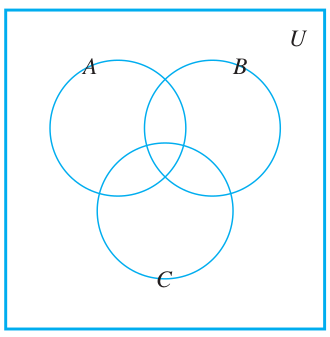
\includegraphics[scale=0.4]{../images/6.2.26.png}
\end{figure}

\subsubsection{(a)}
Illustrate one of the distributive laws by shading in the region corresponding to \(A \cup (B \cap C)\) on one copy 
of the diagram and \((A \cup B) \cap (A \cup C)\) on another.

\begin{proof}
\begin{figure}[ht!]
\centering
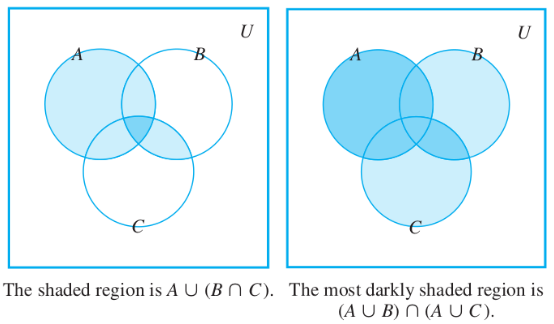
\includegraphics[scale=0.5]{../images/6.2.26.a.png}
\end{figure}
\end{proof}

\subsubsection{(b)}
Illustrate the other distributive law by shading in the region corresponding to \(A \cap (B \cup C)\) on one copy 
of the diagram and \((A \cap B) \cup (A \cap C)\) on another.

\begin{proof}
\begin{figure}[ht!]
\centering
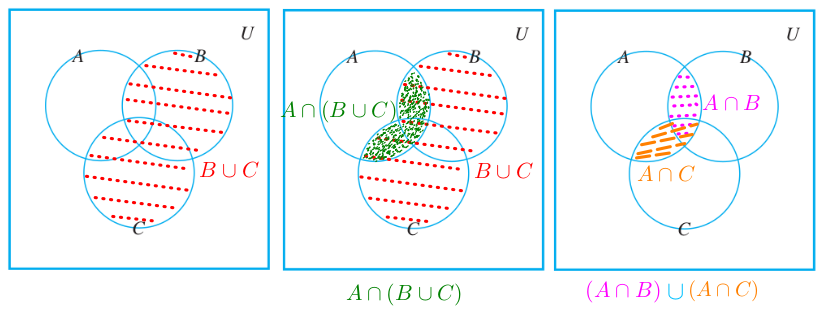
\includegraphics[scale=0.5]{../images/6.2.26.b.png}
\end{figure}
\end{proof}

\subsubsection{(c)}
Illustrate one of De Morgan’s laws by shading in the region corresponding to \((A \cup B)^c\) on one copy of the 
diagram and \(A^c \cap B^c\) on the other. (Leave the set $C$ out of your diagrams.)

\begin{proof}
\begin{figure}[ht!]
\centering
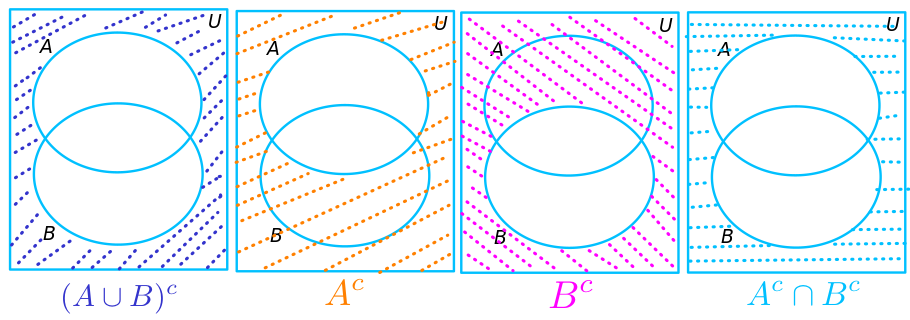
\includegraphics[scale=0.5]{../images/6.2.26.c.png}
\end{figure}
\end{proof}

\subsubsection{(d)}
Illustrate the other De Morgan’s law by shading in the region corresponding to \((A \cap B)^c\) on one copy of the 
diagram and \(A^c \cup B^c\) on the other. (Leave the set $C$ out of your diagrams.)

\begin{proof}
\begin{figure}[ht!]
\centering
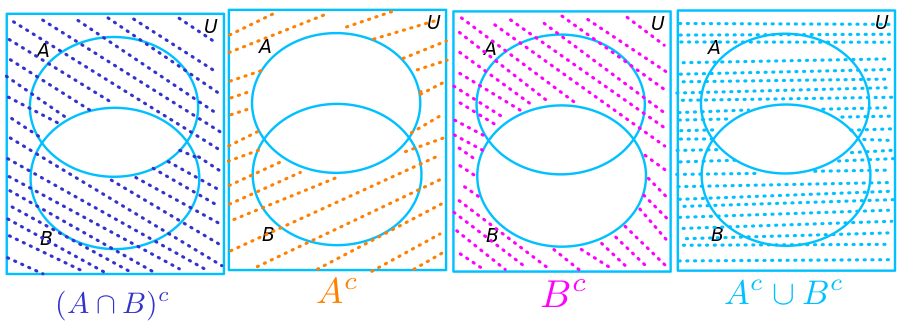
\includegraphics[scale=0.5]{../images/6.2.26.d.png}
\end{figure}
\end{proof}

\subsection{Exercise 27}
Fill in the blanks in the following proof that for all sets $A$ and $B$, \((A - B) \cap (B - A) = \es\).

\underline{Proof:} Let $A$ and $B$ be any sets and suppose \((A - B) \cap (B - A) \neq \es\). That is, suppose there 
is an element $x$ in {\cy (a) \fbl}. By definition of {\cy (b) \fbl}, \(x \in A - B\) and \(x \in {\cy (c) \fbl}\). 
Then by definition of set difference, $x \in A$ and $x \notin B$ and \(x \in {\cy (d) \fbl}\) and \(x \notin {\cy 
(e) \fbl}\). In particular $x \in A$ and \(x \notin {\cy (f) \fbl}\), which is a contradiction. Hence {\it [the 
supposition that \((A - B) \cap (B - A) \neq \es\) is false, and so]} {\cy (g) \fbl}.

\begin{proof}
(a) \((A - B) \cap (B - A)\) (b) intersection (c) $B - A$ (d) $B$ (e) $A$ (f) $A$ (g) \((A - B) \cap (B - A) = \es\)
\end{proof}

{\bf \cy Use the element method for proving a set equals the empty set to prove each statement in $28-38$. Assume that all sets are subsets of a universal set $U$.}

\subsection{Exercise 28}
For all sets $A$ and $B$, \((A \cap B) \cap (A \cap B^c) = \es)\). (This property is used in Section 9.9.)

\begin{proof}
{\it By contradiction:} Suppose not. That is, suppose there exist sets $A$ and $B$ such that \((A \cap B) \cap (A 
\cap B^c) \neq \es\). Then there is an element $x$ in \((A \cap B) \cap (A \cap B^c)\). By definition of intersection, 
\(x \in (A \cap B)\) and \(x \in (A \cap B^c)\). Applying the definition of intersection again, we have that since 
\(x \in (A \cap B), x \in A\) and \(x \in B\), and since \(x \in (A \cap B^c), x \in A\) and \(x \notin B\). Thus, in 
particular, \(x \in B\) and \(x \notin B\), which is a contradiction. It follows that the supposition is false, 
and so \((A \cap B) \cap (A \cap B^c) = \es\).
\end{proof}

\subsection{Exercise 29}
For all sets $A$, $B$, and $C$, \((A - C) \cap (B - C) \cap (A - B) = \es\).

\begin{proof}
{\it By contradiction:} Suppose not. That is, suppose there exist sets $A, B$ and $C$ such that \((A - C) \cap (B - C) 
\cap (A - B) \neq \es\). Then there is an element $x$ in \((A - C) \cap (B - C) \cap (A - B)\). By definition of 
intersection, \(x \in (A - C)\), \(x \in (B - C)\) and \(x \in (A - B)\). Applying the definition of difference, we 
have that since \(x \in (B - C), x \in B\) and \(x \notin C\), and since \(x \in (A - B), x \in A\) and \(x \notin 
B\). Thus, in particular, \(x \in B\) and \(x \notin B\), which is a contradiction. It follows that the supposition 
is false, and so \((A - C) \cap (B - C) \cap (A - B) = \es\).
\end{proof}

\subsection{Exercise 30}
For every subset $A$ of a universal set $U$, \(A \cap A^c = \es\).

\begin{proof}
Let $A$ be a subset of a universal set $U$. Suppose \(A \cap A^c \neq \es\), that is, suppose there is an element 
$x$ such that \(x \in A \cap A^c\). By definition of intersection, $x \in A$ and $x \in A^c$, and so by 
definition of complement, $x \in A$ and $x \notin A$. This is a contradiction. {\it [Hence the supposition is false, 
and we conclude that \(A \cap A^c = \es\).]}
\end{proof}

\subsection{Exercise 31}
If $U$ denotes a universal set, then \(U^c = \es\).

\begin{proof}
Suppose \(U^c \neq \es\), that is, suppose there is an element $x$ such that \(x \in U^c\). By definition of 
complement, $x \notin U$. But by definition of universal set, $x \in U$. This is a contradiction. {\it [Hence the 
supposition is false, and we conclude that \(U^c = \es\).]}
\end{proof}

\subsection{Exercise 32}
For every set $A$, \(A \times \es = \es\).

\begin{proof}
Let $A$ be a set. Suppose \(A \times \es \neq \es\). Then there would be an element $(x, y)$ in \(A \times \es\). By 
definition of Cartesian product, \(x \in A\) and \(y \in \es\). But there are no elements $y$ such that 
\(y \in \es\). Hence there are no elements \((x, y)\) in \(A \times \es\), which is a contradiction. {\it [Thus the 
supposition is false, and so \(A \times \es = \es\).]}
\end{proof}

\subsection{Exercise 33}
For all sets $A$ and $B$, if \(A \subseteq B\) then \(A \cap B^c = \es\).

\begin{proof}
Let $A$ and $B$ be sets such that \(A \subseteq B\). {\it [We must show that \(A \cap B^c = \es\).]} Suppose \(A \cap 
B^c \neq \es\); that is, suppose there were an element $x$ such that \(x \in A \cap B^c\). Then \(x \in A\) and 
\(x \in B^c\) by definition of intersection. So \(x \in A\) and \(x \notin B\) by definition of complement. But 
\(A \subseteq B\) by hypothesis, and, since \(x \in A\), then \(x \in B\) by definition of subset. Thus 
\(x \notin B\) and also \(x \in B\), which is a contradiction. Hence the supposition that \(A \cap B^c \neq 
\es\) is false, and so \(A \cap B^c = \es\).
\end{proof}

\subsection{Exercise 34}
For all sets $A$ and $B$, if \(B \subseteq A^c\) then \(A \cap B = \es\).

\begin{proof}
Let $A$ and $B$ be sets such that \(B \subseteq A^c\). {\it [We must show that \(A \cap B = \es\).]} Suppose \(A \cap B 
\neq \es\); that is, suppose there were an element $x$ such that \(x \in A \cap B\). Then \(x \in A\) and \(x \in B\) 
by definition of intersection. But \(B \subseteq A^c\) by hypothesis, and, since \(x \in B\), then \(x \in A^c\) by 
definition of subset. Thus \(x \notin A\) by definition of complement, and also \(x \in A\), which is a contradiction. 
Hence the supposition that \(A \cap B \neq \es\) is false, and so \(A \cap B = \es\).
\end{proof}

\subsection{Exercise 35}
For all sets $A$, $B$, and $C$, if \(A \subseteq B\) and \(B \cap C = \es\) then \(A \cap C = \es\).

\begin{proof}
Let $A,B$ and $C$ be sets such that \(A \subseteq B\) and \(B \cap C = \es\). {\it [We must show that \(A \cap C = 
\es\).]} Suppose \(A \cap C \neq \es\); that is, suppose there were an element $x$ such that \(x \in A \cap C\). 
Then \(x \in A\) and \(x \in C\) by definition of intersection. But \(A \subseteq B\) by hypothesis, and, 
since \(x \in A\), then \(x \in B\) by definition of subset. Thus \(x \in B\) and also \(x \in C\), so by 
definition of intersection \(x \in B \cap C\), which is a contradiction to the fact that \(B \cap C = \es\). Hence 
the supposition that \(A \cap C \neq \es\) is false, and so \(A \cap C = \es\).
\end{proof}

\subsection{Exercise 36}
For all sets $A$, $B$, and $C$, if \(C \subseteq B - A\) then \(A \cap C = \es\).

\begin{proof}
Let $A$, $B$, and $C$ be any sets such that \(C \subseteq B - A\). Suppose \(A \cap C \neq \es\). Then there is an 
element $x$ such that \(x \in A \cap C\). By definition of intersection, \(x \in A\) and \(x \in C\). Now since \(x 
\in C\) and \(C \subseteq B - A\), then \(x \in B\) and \(x \notin A\). So \(x \in A\) and \(x \notin A\), which is a 
contradiction. Hence the supposition is false, and thus \(A \cap C = \es\).
\end{proof}

\subsection{Exercise 37}
For all sets $A$, $B$, and $C$, if \(B \cap C \subseteq A\), then \((C - A) \cap (B - A) = \es\).

\begin{proof}
Let $A$, $B$, and $C$ be any sets such that \(B \cap C \subseteq A\). Suppose \((C-A) \cap (B-A) \neq \es\). Then 
there is an element $x$ such that \(x \in (C-A) \cap (B-A)\). By definition of intersection, \(x \in C-A\) and \(x 
\in B-A\). Applying the definition of difference, \(x \in C\) and \(x \notin A\), and \(x \in B\) and \(x \notin A\). 
By definition of intersection, \(x \in B \cap C\). By definition of subset, \(x \in A\). So \(x \in A\) and \(x 
\notin A\), which is a contradiction. Hence the supposition is false, and thus \((C-A) \cap (B-A) = \es\).
\end{proof}

\subsection{Exercise 38}
For all sets $A$, $B$, $C$, and $D$, if \(A \cap C = \es\) then \((A \times B) \cap (C \times D) = \es\).

\begin{proof}
Let $A, B, C$ and $D$ be any sets such that \(A \cap C = \es\). Suppose \((A \times B) \cap (C \times D) \neq \es\). 
Then there is an element $(x, y)$ such that \((x,y) \in (A \times B) \cap (C \times D)\). By definition of 
intersection, \((x,y) \in A \times B\) and \((x,y) \in C \times D\). By definition of Cartesian product, \(x \in A\) 
and \(x \in C\). By definition of intersection, \(x \in A \cap C\), which is a contradiction to the fact that \(A 
\cap C = \es\). Hence the supposition is false, and thus \((A \times B) \cap (C \times D) = \es\).
\end{proof}

{\bf \cy Prove each statement in $39-44$.}

\subsection{Exercise 39}
For all sets $A$ and $B$,

\subsubsection{(a)}
\((A - B) \cup (B - A) \cup (A \cap B) = A \cup B\)

\begin{proof}
Start of proof that \(A \cup B \subseteq (A-B) \cup (B-A) \cup (A \cap B)\): 

Given any element $x$ in \(A \cup B\), by definition of union $x$ is in at least one of $A$ and $B$. Thus $x$ 
satisfies exactly one of the following three conditions: 

(1) \(x \in A\) and \(x \notin B\) ($x$ is in $A$ only) 

(2) \(x \in B\) and \(x \notin A\) ($x$ is in $B$ only) 

(3) \(x \in A\) and \(x \in B\) ($x$ is in both $A$ and $B$)
\end{proof}

\subsubsection{(b)}
The sets \((A - B), (B - A), (A \cap B)\) are mutually disjoint.

\begin{proof}
To show that \((A - B), (B - A)\), and \((A \cap B)\) are mutually disjoint, we must show that the intersection of 
any two of them is the empty set. Now, by definition of set difference and set intersection, 

saying that \(x \in A - B\) means that (1) \(x \in A\) and \(x \notin B\), 

saying that \(x \in B - A\) means that (2) \(x \in B\) and \(x \notin A\), and 

saying that \(x \in A \cap B\) means that (3) \(x \in A\) and \(x \in B\). 

Conditions (1)–(3) are mutually exclusive: no two of them can be satisfied at the same time. Thus no element can be 
in the intersection of any two of the sets, and, therefore, the intersection of any two of the sets is the empty set. 

Hence, \((A - B), (B - A)\), and \((A \cap B)\) are mutually disjoint.
\end{proof}

\subsection{Exercise 40}
For every positive integer $n$, if $A$ and \(B_1, B_2, B_3, \ldots\) are any sets, then
\[
A \cap \left(\bigcup_{i=1}^n B_i\right) = \bigcup_{i=1}^n (A \cap B_i).
\]
\begin{proof}
Suppose that $n$ is any positive integer and that $A$ and \(B_1, B_2, B_3, \ldots\) are any sets.

{\bf Proof that} \(\bm{A \cap \left(\bigcup_{i=1}^n B_i\right) \subseteq \bigcup_{i=1}^n (A \cap B_i):}\) 

Suppose $x$ is any element in \(\dps A \cap \left( \bigcup_{i=1}^n B_i\right)\). 
{\it [We must show that \(\dps x \in \bigcup_{i=1}^n (A \cap B_i)\).]}

By definition of intersection, $x \in A$ and \(\dps x \in \bigcup_{i=1}^n B_i\). Since \(\dps x \in \bigcup_{i=1}^n 
B_i\), the definition of general union implies that \(x \in B_i\) for some \(i = 1, 2, \ldots, n\), and so, since \(x 
\in A\), the definition of intersection implies that \(x \in A \cap B_i\). Thus, by definition of general union, 
\(\dps x \in \bigcup_{i=1}^n (A \cap B_i)\) {\it [as was to be shown]}.

{\bf Proof that} \(\bm{\bigcup_{i=1}^n (A \cap B_i) \subseteq A \cap \left(\bigcup_{i=1}^n B_i\right):}\) 

Suppose $x$ is any element in \(\dps \bigcup_{i=1}^n (A \cap B_i)\). 
{\it [We must show that \(\dps x \in A \cap \left( \bigcup_{i=1}^n B_i\right)\).]}

By definition of general union, \(x \in A \cap B_i\) for some \(i = 1, 2, \ldots, n\). Thus, by definition of 
intersection, \(x \in A\) and \(x \in B_i\). Since \(x \in B_i\) for some \(i = 1, 2, \ldots, n\), then by definition 
of general union, \(\dps x \in \bigcup_{i=1}^n B_i\). Thus we have that \(x \in A\) and \(\dps x \in \bigcup_{i=1}^n 
B_i\), and so, by definition of intersection, \(\dps x \in A \cap \bigcup_{i=1}^n B_i\), {\it [as was to be shown].} 

{\bf Conclusion:} Since both subset relations have been proved, it follows by definition of set equality that 
\[
A \cap \left(\bigcup_{i=1}^n B_i\right) = \bigcup_{i=1}^n (A \cap B_i).
\]
\end{proof}

\subsection{Exercise 41}
For every positive integer $n$, if \(A_1, A_2, A_3, \ldots\) and $B$ are any sets, then
\[
\bigcup_{i=1}^n (A_i - B) = \left(\bigcup_{i=1}^n A_i\right) - B.
\]
\begin{proof}
Assume $n$ is a positive integer, \(A_1, A_2, A_3, \ldots\) and $B$ are any sets.

1. Assume \(\dps x \in \bigcup_{i=1}^n (A_i - B)\). {\it [Want to show \(\dps x \in \left(\bigcup_{i=1}^n A_i\right) - B\)].}

2. By 1 and definition of \(\dps \bigcup\), there exists a $j$ in \(\{1, \ldots, n\}\) such that \(x \in A_j - B\).

3. By 2 and definition of difference, \(x \in A_j\) and \(x \notin B\).

4. By 3 and definition of $\dps \bigcup$, \(\dps x \in \bigcup_{i=1}^n A_i\).

5. By 3 and 4 and definition of difference, \(\dps x \in \left(\bigcup_{i=1}^n A_i\right) - B\).

6. By 1 and 5 and definition of subset, \(\dps \bigcup_ {i=1}^n (A_i - B) \subseteq \left(\bigcup_{i=1}^n A_i\right) - B.\)

{\bf Now the reverse part:}

7. Assume \(\dps x \in \left(\bigcup_{i=1}^n A_i\right) - B\). {\it [Want to show \(\dps x \in \bigcup_{i=1}^n (A_i - B)\)].}

8. By 7 and definition of difference, \(\dps x \in \bigcup_{i=1}^n A_i\) and \(x \notin B\).

9. By 8 and definition of $\dps \bigcup$, there exists $j$ in \(\{1, \ldots, n\}\) such that \(x \in A_j\).

10. By 8 and 9 and definition of difference, \(x \in A_j - B\).

11. By 10 and definition of $\dps \bigcup$, \(x \in \dps \bigcup_{i=1}^n (A_i - B)\).

12. By 11 and 7 and definition of subset, \(\dps \left( \bigcup_{i=1}^n A_i\right) - B \subseteq \bigcup_{i=1}^n (A_i - B)\).

{\bf 13. Conclusion:} By 6 and 12 and definition of set equality,
\[
\bigcup_{i=1}^n (A_i - B) = \left(\bigcup_{i=1}^n A_i\right) - B.
\] 
\end{proof}

\subsection{Exercise 42}
For every positive integer $n$, if \(A_1, A_2, A_3, \ldots\) and $B$ are any sets, then
\[
\bigcap_{i=1}^n (A_i - B) = \left(\bigcap_{i=1}^n A_i\right) - B.
\]
\begin{proof}
Assume $n$ is a positive integer, \(A_1, A_2, A_3, \ldots\) and $B$ are any sets.

1. Assume \(\dps x \in \bigcap_{i=1}^n (A_i - B)\). {\it [Want to show \(\dps x \in \left(\bigcap_{i=1}^n A_i\right) - B\)].}

2. By 1 and definition of \(\dps \bigcap\), \(x \in A_i - B\) for all $i$ in \(\{1, \ldots, n\}\).

3. By 2 and definition of difference, \(x \in A_i\) for all $i$ in \(\{1, \ldots, n\}\), and \(x \notin B\).

4. By 3 and definition of $\dps \bigcap$, \(\dps x \in \bigcap_{i=1}^n A_i\).

5. By 3 and 4 and definition of difference, \(\dps x \in \left(\bigcap_{i=1}^n A_i\right) - B\).

6. By 1 and 5 and definition of subset, \(\dps \bigcap_ {i=1}^n (A_i - B) \subseteq \left(\bigcap_{i=1}^n A_i\right) - B.\)

{\bf Now the reverse part:}

7. Assume \(\dps x \in \left(\bigcap_{i=1}^n A_i\right) - B\). {\it [Want to show \(\dps x \in \bigcap_{i=1}^n (A_i - B)\)].}

8. By 7 and definition of difference, \(\dps x \in \bigcap_{i=1}^n A_i\) and \(x \notin B\).

9. By 8 and definition of $\dps \bigcap$, \(x \in A_i\) for all $i$ in \(\{1, \ldots, n\}\).

10. By 8 and 9 and definition of difference, \(x \in A_i - B\) for all $i$ in \(\{1, \ldots, n\}\).

11. By 10 and definition of $\dps \bigcap$, \(x \in \dps \bigcap_{i=1}^n (A_i - B)\).

12. By 11 and 7 and definition of subset, \(\dps \left( \bigcap_{i=1}^n A_i\right) - B \subseteq \bigcap_{i=1}^n (A_i - B)\).

{\bf 13. Conclusion:} By 6 and 12 and definition of set equality,
\[
\bigcap_{i=1}^n (A_i - B) = \left(\bigcap_{i=1}^n A_i\right) - B.
\]
\end{proof}

\subsection{Exercise 43}
For every positive integer $n$, if $A$ and \(B_1, B_2, B_3, \ldots\) are any sets, then
\[
\bigcup_{i=1}^n (A \times B_i) = A \times \left( \bigcup_{i=1}^n B_i\right).
\]
\begin{proof}
Assume $n$ is a positive integer, \(B_1, B_2, B_3, \ldots\) and $A$ are any sets.

1. Assume \(\dps (x,y) \in \bigcup_{i=1}^n (A \times B_i)\). {\it [Want to show \(\dps (x,y) \in A \times \left( 
\bigcup_{i=1}^n B_i\right)\)].}

2. By 1 and definition of \(\dps \bigcup\), there exists a $j$ in \(\{1, \ldots, n\}\) such that \((x,y) \in A \times B_j\).

3. By 2 and definition of Cartesian product, \(x \in A\) and \(y \in B_j\).

4. By 3 and definition of $\dps \bigcup$, \(\dps y \in \bigcup_{i=1}^n B_i\).

5. By 3 and 4 and definition of Cartesian product, \(\dps (x,y) \in A \times \left(\bigcup_{i=1}^n B_i\right)\).

6. By 1 and 5 and definition of subset, \(\dps \bigcup_ {i=1}^n (A \times B_i) \subseteq A \times \left(
\bigcup_{i=1}^n B_i\right).\)

{\bf Now the reverse part:}

7. Assume \(\dps (x,y) \in A \times \left(\bigcup_{i=1}^n B_i\right)\). 
{\it [Want to show \(\dps (x,y) \in \bigcup_{i=1}^n (A \times B_i)\)].}

8. By 7 and definition of Cartesian product, \(x \in A \) and \(\dps y \in \bigcup_{i=1}^n B_i\).

9. By 8 and definition of $\dps \bigcup$, there exists $j$ in \(\{1, \ldots, n\}\) such that \(y \in B_j\).

10. By 8 and 9 and definition of Cartesian product, \((x,y) \in A \times B_j\).

11. By 10 and definition of $\dps \bigcup$, \((x, y) \in \dps \bigcup_{i=1}^n (A \times B_i)\).

12. By 11 and 7 and definition of subset, \(\dps A \times \left(\bigcup_{i=1}^n B_i\right) \subseteq \bigcup_{i=1}^n (A \times B_i)\).

{\bf 13. Conclusion:} By 6 and 12 and definition of set equality,
\[
A \times \left(\bigcup_{i=1}^n B_i\right) = \bigcup_{i=1}^n (A \times B_i).
\]
\end{proof}

\subsection{Exercise 44}
For every positive integer $n$, if $A$ and \(B_1, B_2, B_3, \ldots\) are any sets, then
\[
\bigcap_{i=1}^n (A \times B_i) = A \times \left( \bigcap_{i=1}^n B_i\right).
\]
\begin{proof}
Assume $n$ is a positive integer, \(B_1, B_2, B_3, \ldots\) and $A$ are any sets.

1. Assume \(\dps (x,y) \in \bigcap_{i=1}^n (A \times B_i)\). 
{\it [Want to show \(\dps (x,y) \in A \times \left(\bigcap _{i=1}^n B_i\right)\)].}

2. By 1 and definition of \(\dps \bigcap\), \((x,y) \in A \times B_i\) for all $i$ in \(\{1, \ldots, n\}\).

3. By 2 and definition of Cartesian product, \(x \in A\) and \(y \in B_i\) for all $i$ in \(\{1, \ldots, n\}\).

4. By 3 and definition of $\dps \bigcap$, \(\dps y \in \bigcap_{i=1}^n B_i\).

5. By 3 and 4 and definition of Cartesian product, \(\dps (x, y) \in A \times \left(\bigcap_{i=1}^n B_i\right)\).

6. By 1 and 5 and definition of subset, \(\dps \bigcap _{i=1}^n (A \times B_i) \subseteq A \times \left(
\bigcap _{i=1}^n B_i\right).\)

{\bf Now the reverse part:}

7. Assume \(\dps (x,y) \in A \times \left( \bigcap_{i=1}^n B_i\right)\). {\it [Want to show \(\dps x \in \bigcap _{i=1}^n (A \times B_i)\)].}

8. By 7 and definition of Cartesian product, \(x \in A\) and \(\dps y \in \bigcap_{i=1}^n B_i\).

9. By 8 and definition of $\dps \bigcap$, \(y \in B_i\) for all $i$ in \(\{1, \ldots, n\}\).

10. By 8 and 9 and definition of Cartesian product, \((x,y) \in A \times B_i\) for all $i$ in \(\{1, \ldots, n\}\).

11. By 10 and definition of $\dps \bigcap$, \((x,y) \in \dps \bigcap_{i=1}^n (A \times B_i)\).

12. By 11 and 7 and definition of subset, \(\dps A \times \left(\bigcap_{i=1}^n B_i\right) \subseteq \bigcap_{i=1}^n 
(A \times B_i)\).

{\bf 13. Conclusion:} By 6 and 12 and definition of set equality,
\[
\bigcap_{i=1}^n (A \times B_i) = A \times \left( \bigcap_{i=1}^n B_i\right).
\]
\end{proof}

\section{Exercise Set 6.3}

{\bf \cy For each of $1-4$ find a counterexample to show that the statement is false. Assume all sets are subsets of a universal set $U$.}

\subsection{Exercise 1}
For all sets $A$, $B$, and $C$, \((A \cup B) \cap C = A \cup (B \cap C)\).

\begin{proof}
\underline{Counterexample:} $A$, $B$, and $C$ can be any sets where $A$ has an element that is not in $C$. For 
instance, let \(A = \{1, 2\}, B = \{2\}\), and \(C = \{2\}\). Then \((A \cup B) \cap C = (\{1, 2\} \cup \{2\}) \cap 
\{2\} = \{1, 2\} \cap \{2\} = \{2\}\), and \(A \cup (B \cap C) = \{1, 2\} \cup (\{2\} \cap \{2\}) = \{1, 2\} \cup \{2\} 
= \{1, 2\}\). Thus \(1 \in A \cup (B \cap C)\) but \(1 \notin (A \cup B) \cap C\), and hence \((A \cup B) \cap C 
\neq A \cup (B \cap C)\) by definition of subset.
\end{proof}

\subsection{Exercise 2}
For all sets $A$, $B$, \((A \cup B)^c = A^c \cup B^c\).

\begin{proof}
Let \(U = \{1, 2\}, A = \{1\}, B = \{2\}\). Then \(A \cup B = \{1, 2\}\) so \((A \cup B)^c = \es\). But \(A^c = \{2\}, 
B^c = \{1\}\) and so \(A^c \cup B^c = \{1, 2\} \neq \es = (A \cup B)^c\).
\end{proof}

\subsection{Exercise 3}
For all sets $A$, $B$, and $C$, if \(A \nsubseteq B\) and \(B \nsubseteq C\) then \(A \nsubseteq C\).

\begin{proof}
\underline{Counterexample:} $A$, $B$, and $C$ can be any sets where \(A \subseteq C\) and $B$ contains at least one 
element that is not in either $A$ or $C$. For instance, let \(A = \{1\}, B = \{2\}\), and \(C = \{1, 3\}\). Then 
\(A \nsubseteq B\) and \(B \nsubseteq C\) but \(A \subseteq C\).
\end{proof}

\subsection{Exercise 4}
For all sets $A$, $B$, and $C$, if \(B \cup C \subseteq A\) then \((A - B) \cap (A - C) = \es\).

\begin{proof}
Let \(A = \{1, 2, 3\}, B = \{2\}, C = \{3\}\). Then \(B \cup C = \{2, 3\} \subseteq A\). And \(A - B = \{1, 3\}\)
and \(A - C = \{1, 2\}\), but \((A - B) \cap (A - C) = \{1, 3\} \cap \{1, 2\} = \{1\} \neq \es\).
\end{proof}

{\bf \cy For each of $5-21$ prove each statement that is true and find a counterexample for each statement that is false. Assume all sets are subsets of a universal set $U$.}

\subsection{Exercise 5}
For all sets $A$, $B$, and $C$, \(A - (B - C) = (A - B) - C\).

\begin{proof}
False. \underline{Counterexample:} $A$, $B$, and $C$ can be any sets where all three sets have an element in common or 
where $A$ and $C$ have a common element that is not in $B$. For instance, let \(A = \{1, 2, 3\}, B = \{2, 3\}\), and 
\(C = \{3\}\). Then \(B - C = \{2\}\), and so \(A - (B - C) = \{1, 2, 3\} - \{2\} = \{1, 3\}\). On the other hand, 
\(A - B = \{1, 2, 3\} - \{2, 3\} = \{1\}\), and so \((A - B) - C = \{1\} - \{3\} = \{1\}\). 
Since \(\{1, 3\} \neq \{1\}\), \(A-(B-C) \neq (A-B)-C\).
\end{proof}

\subsection{Exercise 6}
For all sets $A$, $B$, \(A \cap (A \cup B) = A\).

\begin{proof}
True. Let $A$ and $B$ be any sets. 

{\bf Proof that \(\bm{A \cap (A \cup B) \subseteq A}\):} Suppose \(x \in A \cap (A \cup B)\). By definition of 
intersection, $x \in A$ and \(x \in A \cup B\). In particular, $x \in A$. Thus, by definition of subset, 
\(A \cap (A \cup B) \subseteq A\). 

{\bf Proof that \(\bm{A \subseteq A \cap (A \cup B)}\):} Suppose $x \in A$. Then by definition of union, \(x \in A \cup B\). 
Hence $x \in A$ and \(x \in A \cup B\), and so, by definition of intersection \(x \in A \cap (A \cup B)\). 
Thus, by definition of subset, \(A \subseteq A \cap (A \cup B)\). 

Because both \(A \cap (A \cup B) \subseteq A\) and \(A \subseteq A \cap (A \cup B)\) have been proved, we conclude 
that \(A \cap (A \cup B) = A\).
\end{proof}

\subsection{Exercise 7}
For all sets $A$, $B$, and $C$, \((A - B) \cap (C - B) = A - (B \cup C)\).

\begin{proof}
\underline{Counterexample:} 
Let \(A = \{1\}, B = \{2\}, C = \{3\}\). Then \(A-B= \{1\}, C - B = \{3\}, B \cup C = \{2, 3\}\). 
So \((A - B) \cap (C - B) = \{1\} \cap \{3\} = \es \neq \{1\} = A - (B \cup C)\).
\end{proof}

\subsection{Exercise 8}
For all sets $A$, $B$, and $C$, if \(A^c \subseteq B\) then \(A \cup B = U\).

\begin{proof}
Assume \(x \in A \cup B\). By definition of universal set, \(x \in U\). 
So by definition of subset, \(A \cup B \subseteq U\).

Assume \(x \in U\). There are two cases: $x \in A$ or $x \notin A$. 

In the first case, $x \in A \cup B$ by definition of union. 

In the second case, $x \in A^c$ by definition of complement, and so $x \in B$ because \(A^c \subseteq B\). 
Since $x \in B$, then \(x \in A \cup B\) by definition of union.

In both cases \(x \in A \cup B\). So by definition of subset, \(U \subseteq A \cup B\).

By definition of set equality, \(A \cup B = U\).
\end{proof}

\subsection{Exercise 9}
For all sets $A$, $B$, and $C$, if \(A \subseteq C\) and \(B \subseteq C\) then \(A \cup B \subseteq C\).

\begin{proof}
True. Suppose $A, B$, and $C$ are any sets such that \(A \subseteq C\) and \(B \subseteq C\). Let \(x \in A \cup B\). 
By definition of union, \(x \in A\) or \(x \in B\). But if \(x \in A\) then \(x \in C\) (because \(A \subseteq C\)), 
and if \(x \in B\) then \(x \in C\) (because \(B \subseteq C\)). Hence, in either case, \(x \in C\). {\it [So, by 
definition of subset, \(A \cup B \subseteq C\).]}
\end{proof}

\subsection{Exercise 10}
For all sets $A$, $B$, if \(A \subseteq B\) then \(A \cap B^c = \es\).

\begin{proof}
Argue by contradiction and assume \(A \cap B^c \neq \es\).
There exists $x$ such that \(x \in A \cap B^c \). By definition of intersection, $x \in A$ and $x \in B^c$.
Since \(A \subseteq B\) and \(x \in A\), \(x \in B\). Since $x \in B^c$, by definition of complement \(x \notin B\).
So both \(x \in B\) and \(x \notin B\), contradiction.
Therefore \(A \cap B^c = \es\).
\end{proof}

\subsection{Exercise 11}
For all sets $A$, $B$, and $C$, if \(A \subseteq B\) then \(A \cap (B \cap C)^c = \es\).

\begin{proof}
The statement is false. Let \(U = \{1, 2, 3, 4\}, A = \{1, 2\}, B = \{1, 2, 3\}, C = \{2\}\).

Notice that \(A = \{1, 2\} \subseteq \{1, 2, 3\} = B\). And \(B \cap C = \{1, 2, 3\} \cap \{2\} = \{2\}\), so 
\((B \cap C)^c = \{1, 3, 4\}\) but \(A \cap (B \cap C)^c = \{1, 2\} \cap \{1, 3, 4\} = \{1\} \neq \es\).
\end{proof}

\subsection{Exercise 12}
For all sets $A$, $B$, and $C$, \(A \cap (B - C) = (A \cap B) - (A \cap C)\).

\begin{proof}
1. Assume \(x \in A \cap (B - C)\).

2. By 1 and definition of intersection \(x \in A\) and \(x \in (B - C)\).

3. By 2 and definition of difference, \(x \in B\) and \(x \notin C\).

4. By 2 and 3 and definition of intersection, \(x \in A \cap B\).

5. If \(x \in A \cap C\) then by definition of intersection \(x \in C\), contradiction to 3. Thus \(x \notin A \cap C\). 

6. By 4 and 5 and definition of difference, \(x \in (A \cap B) - (A \cap C)\).

7. By 1 and 6 and definition of subset, \(A \cap (B - C) \subseteq (A \cap B) - (A \cap C)\).

{\bf Now the reverse part:}

8. Assume \(x \in (A \cap B) - (A \cap C)\).

9. By 8 and definition of difference, \(x \in (A \cap B)\) and \(x \notin (A \cap C)\).

10. By 9 and definition of intersection, \(x \in A\) and \(x \in B\).

11. If \(x \in C\) then by 10 and definition of intersection, \(x \in A \cap C\), contradiction to 9. 
Thus \(x \notin C\).

12. By 10 and 11 and definition of difference, \(x \in B - C\).

13. By 10 and 12 and definition of intersection, \(x \in A \cap (B - C)\).

14. By 8 and 13 and definition of subset, \((A \cap B) - (A \cap C) \subseteq A \cap (B - C)\).

{\bf Conclusion:} By 7 and 14 and definition of set equality, \((A \cap B) - (A \cap C) = A \cap (B - C)\).
\end{proof}

\subsection{Exercise 13}
For all sets $A$, $B$, and $C$, \(A \cup (B - C) = (A \cup B) - (A \cup C)\).

\begin{proof}
False. Let \(A = \{1\}, B = \{2\}, C = \{3\}\). Then \(A \cup (B - C) = \{1\} \cup (\{2\} - \{3\}) = \{1\} \cup 
\{2\} = \{1, 2\}\), and \((A \cup B) - (A \cup C) = (\{1\} \cup \{2\}) - (\{1\} \cup \{3\}) = \{1, 2\} - \{1, 3\} = 
\{2\}\). But \(\{1, 2\} \neq \{2\}\).
\end{proof}

\subsection{Exercise 14}
For all sets $A$, $B$, and $C$, if \(A \cap C = B \cap C\) and \(A \cup C = B \cup C\), then $A = B$.

\begin{proof}
The statement is true. 

1. Suppose \(x \in A\). {\it [We must show that \(x \in B\).]}

2. Either \(x \in C\) or \(x \notin C\). 

3. In case \(x \in C\), by 1 and definition of intersection \(x \in A \cap C = B \cap C\). 
Then by definition of intersection, \(x \in B\). 

4. In case \(x \notin C\), by 1 and definition of intersection \(x \in A \cup C = B \cup C\). 
Then by definition of union \(x \in B\) or \(x \in C\), therefore \(x \in B\).

5. By 1, 4 and definition of subset, \(A \subseteq B\).

6. Suppose \(x \in B\). {\it [We must show that \(x \in A\).]}

7. Either \(x \in C\) or \(x \notin C\). 

8. In case \(x \in C\), by 6 and definition of intersection \(x \in B \cap C = A \cap C\). 
Then by definition of intersection, \(x \in A\). 

9. In case \(x \notin C\), by 6 and definition of intersection \(x \in B \cup C = A \cup C\). 
Then by definition of union \(x \in A\) or \(x \in C\), therefore \(x \in A\).

10. By 6, 9 and definition of subset, \(B \subseteq A\).

11. By 5, 10 and definition of set equality, $A = B$.
\end{proof}

\subsection{Exercise 15}
For all sets $A$, $B$, and $C$, \((A - B) \cup C \subseteq A \cup (C - B)\).

\begin{proof}
False. \underline{Counterexample:} Let \(A = \{1, 2\}, B = \{2, 3\}, C = \{3, 4\}\). 

Then \((A - B) \cup C = (\{1, 2\} - \{2, 3\}) \cup \{3, 4\} = \{1\} \cup \{3, 4\} = \{1, 3, 4\}\). 

And \(A \cup (C - B) = \{1, 2\} \cup (\{3, 4\} - \{2, 3\}) = \{1, 2\} \cup \{4\} = \{1, 2, 4\}\). 

But \(\{1, 3, 4\} \nsubseteq \{1, 2, 4\}\).
\end{proof}

\subsection{Exercise 16}
For all sets $A$, $B$, if \(A \cap B = \es\) then \(A \times B = \es\).

\begin{proof}
False. \underline{Counterexample:} Let \(A = \{1\}, B = \{2\}\). 
Then \(A \cap B = \es\) but \(A \times B = \{(1, 2)\} \neq \es\).
\end{proof}

\subsection{Exercise 17}
For all sets $A$, $B$, if \(A \subseteq B\) then \(\ps(A) \subseteq \ps(B)\).

\begin{proof}
Suppose $A$ and $B$ are any sets with \(A \subseteq B\). {\it [We must show that \(\ps(A) \subseteq \ps(B)\).]} 
So suppose \(X \in \ps(A)\). Then \(X \subseteq A\) by definition of power set. And because \(A \subseteq B\), 
we also have that \(X \subseteq B\) by the transitive property for subsets. Thus, by definition of power set, 
\(X \in \ps(B)\). This proves that for all $X$, if \(X \in \ps(A)\) then \(X \in \ps(B)\), and so 
\(\ps(A) \subseteq \ps(B)\), {\it [as was to be shown]}.
\end{proof}

\subsection{Exercise 18}
For all sets $A$, $B$, \(\ps(A \cup B) \subseteq \ps(A) \cup \ps(B)\).

\begin{proof}
False. \underline{Counterexample:} For any sets $A$ and $B$, the only sets in \(\ps(A) \cup \ps(B)\) are subsets of 
either $A$ or $B$, whereas a set in \(\ps(A \cup B)\) can contain elements from both $A$ and $B$. Thus, if at least 
one of $A$ or $B$ contains elements that are not in the other set, \(\ps(A) \cup \ps(B)\) and \(\ps(A \cup B)\) 
will not be equal. For instance, let \(A = \{1\}\) and \(B = \{2\}\). Then \(\{1, 2\} \in \ps(A \cup B)\) but 
\(\{1, 2\} \notin \ps(A) \cup \ps(B)\).
\end{proof}

\subsection{Exercise 19}
For all sets $A$, $B$, \(\ps(A) \cup \ps(B) \subseteq \ps(A \cup B)\).

\begin{proof}
Assume $A$, $B$ are any sets.

1. Assume \(x \in \ps(A) \cup \ps(B)\). {\it [Want to show \(x \in \ps(A \cup B)\)]}.

2. By definition of union \(x \in \ps(A)\) or \(x \in \ps(B)\).

3. Case 1: \(x \in \ps(A)\). By definition of power set, \(x \subseteq A\). By definition of union, \(A \subseteq A 
\cup B\). By transitivity of subsets, \(x \subseteq A \cup B\). By definition of power set, \(x \in \ps(A \cup B)\).

4. Case 2: \(x \in \ps(B)\). By definition of power set, \(x \subseteq B\). By definition of union, \(B \subseteq A 
\cup B\). By transitivity of subsets, \(x \subseteq A \cup B\). By definition of power set, \(x \in \ps(A \cup B)\).

5. By 2, 3, 4, \(x \in \ps(A \cup B)\).

6. By 1, 5 and definition of subset, \(\ps(A) \cup \ps(B) \subseteq \ps(A \cup B)\).
\end{proof}

\subsection{Exercise 20}
For all sets $A$, $B$, \(\ps(A \cap B) = \ps(A) \cap \ps(B)\).

\begin{proof}
1. Assume \(x \in \ps(A \cap B)\). {\it [Want to show \(x \in \ps(A) \cap \ps(B)\).]}

2. By 1 and definition of power set, \(x \subseteq A \cap B\).

3. By 2 and definition of intersection, \(x \subseteq A\) and \(x \subseteq B\).

4. By 3 and definition of power set, \(x \in \ps(A)\) and \(x \in \ps(B)\).

5. By 4 and definition of intersection, \(x \in \ps(A) \cap \ps(B)\).

6. By 1, 5 and definition of subset, \(\ps(A \cap B) \subseteq \ps(A) \cap \ps(B)\).

7. Assume \(x \in \ps(A) \cap \ps(B)\). {\it [Want to show \(x \in \ps(A \cap B)\).]}

8. By 7 and definition of intersection, \(x \in \ps(A)\) and \(x \in \ps(B)\).

9. By 8 and definition of power set, \(x \subseteq A\) and \(x \subseteq B\).

10. By 9 and definition of intersection, \(x \subseteq A \cap B\).

11. By 10 and definition of power set, \(x \in \ps(A \cap B)\).

12. By 7, 11 and definition of subset, \(\ps(A) \cap \ps(B) \subseteq \ps(A \cap B)\).

13. By 6, 12 and definition of set equality, \(\ps(A \cap B) = \ps(A) \cap \ps(B)\).
\end{proof}

\subsection{Exercise 21}
For all sets $A$, $B$, \(\ps(A \times B) = \ps(A) \times \ps(B)\).

\begin{proof}
False. \underline{Counterexample:} Let \(A = \{1\}, B = \{2\}\). Then \(A \times B = \{(1, 2)\}\). 

So \(\ps(A) = 
\{\es, \{1\}\}, \ps(B) = \{\es, \{2\}\}\) and \(\ps(A \times B) = \{\es, \{(1, 2)\}\}\). 

But \(\ps(A) \times \ps(B) = \{(\es, \es), (\es, \{2\}), (\{1\}, \es), (\{1\}, \{2\})\} \neq \{\es, \{(1, 2)\}\}.\)
\end{proof}

\subsection{Exercise 22}
Write a negation for each of the following statements. Indicate which is true, the statement or its negation. 
Justify your answers.

\subsubsection{(a)}
\(\forall\) sets $S$, \(\exists\) a set $T$ such that \(S \cap T = \es\).

\begin{proof}
True. Let $T = S^c$.

\underline{Negation:} \(\exists\) a set $S$ such that \( \forall\) sets $T$, \(S \cap T \neq \es\).
\end{proof}

\subsubsection{(b)}
\(\exists\) a set $S$ such that \(\forall\) sets $T$, \(S \cup T = \es\).

\begin{proof}
False. If $T$ is nonempty, then no choice of $S$ works.

\underline{Negation:} \(\forall\) sets $S$ \(\exists\) a set $T$ such that \(S \cup T \neq \es\).

Negation is true: let $T$ be any nonempty set.
\end{proof}

\subsection{Exercise 23}
Let \(S = \{a, b, c\}\), and for each integer \(i = 0, 1, 2, 3\), let $S_i$ be the set of all subsets of $S$ that 
have $i$ elements. List the elements in \(S_0, S_1, S_2\), and $S_3$. Is \(\{S_0, S_1, S_2, S_3\}\) a partition of $\ps(S)$?

\begin{proof}
\(S_0 = \{\es\}, S_1 = \{\{a\}, \{b\}, \{c\}\}, S_2 = \{\{a,b\}, \{a,c\}, \{b,c\}\}, S_3 = \{\{a,b,c\}\}\).

Yes it is a partition of $\ps(S)$.
\end{proof}

\subsection{Exercise 24}
Let \(A = \{t, u, v, w\}\), and let $S_1$ be the set of all subsets of $A$ that do not contain $w$ and $S_2$ the set of all subsets of $A$ that contain $w$.

\subsubsection{(a)}
Find $S_1$.

\begin{proof}
\(S_1 = \ps(\{t,u,v\}) = \{\es, \{t\}, \{u\}, \{v\}, \{t,u\}, \{t,v\}, \{u,v\}, \{t,u,v\}\}\)
\end{proof}

\subsubsection{(b)}
Find $S_2$.

\begin{proof}
\(S_2 = \{\{w\}, \{t,w\}, \{u,w\}, \{v,w\}, \{t,u,w\}, \{t,v,w\}, \{u,v,w\}, \{t,u,v,w\}\}\)
\end{proof}

\subsubsection{(c)}
Are $S_1$ and $S_2$ disjoint?

\begin{proof}
Yes.
\end{proof}

\subsubsection{(d)}
Compare the sizes of $S_1$ and $S_2$.

\begin{proof}
They are equal (8).
\end{proof}

\subsubsection{(e)}
How many elements are in \(S_1 \cup S_2\)?

\begin{proof}
16.
\end{proof}

\subsubsection{(f)}
What is the relation between \(S_1 \cup S_2\) and \(\ps(A)\)?

\begin{proof}
\(S_1 \cup S_2 = \ps(A)\).
\end{proof}

\subsection{Exercise 25}
Use mathematical induction to prove that for every integer $n \geq 2$, if a set $S$ has $n$ elements, then the number 
of subsets of $S$ with an even number of elements equals the number of subsets of $S$ with an odd number of elements.

\begin{proof}
For the sake of simplicity let's introduce some notation. For a set $S$ define \(even(S)\) = the set of elements of
$S$ with an even number of elements, and \(odd(S)\) = the set of elements of $S$ with an odd number of elements.
(Notice we said ``elements of $S$'' not ``subsets of $S$''.)

Let $P(n)$ be the sentence “If a set $S$ has $n$ elements, then \(|even(\ps(S))| = |odd(\ps(S))|\).” (Here $|a|$ denotes the size of the set $a$.)

{\bf Show that $P(2)$ is true:}

Assume a set $S$ has two elements: \(S = \{a, b\}\). Then \(\ps(S) = \{\es, \{a\}, \{b\}, \{a, b\}\}\). 

There are two subsets with an even number of elements: \(\es\) (which has 0 elements) and \(\{a, b\}\) (which has 2
elements).

There are two subsets with an odd number of elements: \(\{a\}, \{b\}\) (both of which have 1 element).

Since 2 = 2, $P(2)$ is true.

{\bf Show that for any integer $k \geq 2$ if $P(k)$ is true then $P(k+1)$ is true:} Assume “If a set $S$ has $k$ elements, \(|even(\ps(S))| = |odd(\ps(S))|\).”

Assume $X$ is a set with $k+1$ elements. {\it [We want to show \(|even(\ps(X))| = |odd(\ps(X))|\).]} 

Since $k+1 \geq 1$ we may pick an element $z \in X$. Let $S = X - \{z\}$. Then $S$ has $k$ elements, so by inductive hypothesis \(|even(\ps(S))| = |odd(\ps(S))|\).

Observe that any subset of $X$ either contains $z$ or does not. Let $A$ be the set of subsets of $X$ that contain $z$, 
let $B$ be the set of subsets of $X$ that do not contain $z$. 

Notice $A$ and $B$ form a partition of $\ps(X)$, so \(|even(\ps(X))| = |even(A)| + |even(B)|\), and \(|
odd(\ps(X))| = |odd(A)| + |odd(B)|\). Also notice that \(B = \ps(S)\), so \(|even(B)| = |odd(B)|\).

Now consider the following one-to-one correspondence between $A$ and $B$: for any $b \in B$ there is $a \in A$
given by \(a = b \cup \{z\}\). Similarly for any $a \in A$ there is $b \in B$ given by \(b = a - \{z\}\). Then $A$ and
$B$ have the same number of elements.

Notice that under this correspondence, if $b \in B$ has an even number of elements, then \(a = b \cup \{z\}\) has an
odd number of elements, and vice versa. Therefore: \(|even(A)| = |odd(B)|\) and \(|odd(A)| = |even(B)|\). Since
\(|even(B)| = |odd(B)|\), we get \(|even(A)| = |odd(A)|\).

Putting these facts together, we get
\[
|even(\ps(X))| = |even(A)| + |even(B)| = |odd(A)| + |odd(B)| = |odd(\ps(X))|,
\]
{\it [as was to be shown.]}
\end{proof}

\subsection{Exercise 26}
The following problem, devised by Ginger Bolton, appeared in the January 1989 issue of the College Mathematics Journal (Vol. 20, No. 1, p. 68): Given a positive integer $n \geq 2$, let $S$ be the set of all nonempty subsets of \(\{2, 3, \ldots, n\}\). For each \(S_i \in S\), let $P_i$ be the product of the elements of $S_i$. Prove or disprove that
\[
\sum_{i=1}^{2^{n-1}-1} P_i = \frac{(n+1)!}{2} - 1
\]
\begin{proof}
Hint: Use mathematical induction. In the inductive step, you will consider the set of all nonempty subsets of 
\(\{2, \ldots, k\}\) and the set of all nonempty subsets of \(\{2, \ldots, k + 1\}\). Any subset of 
\(\{2, \ldots, k + 1\}\) either contains \(k + 1\) or does not contain \(k + 1\). Thus the sum of all products of 
elements of nonempty subsets of \(\{2, \ldots , k + 1\}\) = the sum of all products of elements of nonempty subsets of 
\(\{2, \ldots, k + 1\}\) that do not contain \(k + 1\) + the sum of all products of elements of nonempty subsets of 
\(\{2, \ldots, k + 1\}\) that contain \(k + 1\) Now any subset of \(\{2, \ldots, k + 1\}\) that does not contain 
\(k + 1\) is a subset of \(\{2, \ldots, k\}\). And any subset of \(\{2, \ldots, k + 1\}\) that contains \(k + 1\) 
is the union of a subset of \(\{2, \ldots, k\}\) and \(\{k + 1\}\).
\end{proof}

{\bf \cy In 27 and 28 supply a reason for each step in the derivation.}

\subsection{Exercise 27}
For all sets $A$, $B$, and $C$, \((A \cup B) \cap C = (A \cap C) \cup (B \cap C)\).

\underline{Proof:} Suppose $A,B,C$ are any sets. Then

\begin{tabular}{rcll}
\((A \cup B) \cap C\) & = & \(C \cap (A \cup B)\) & by (a) \fbl \\
& = & \((C \cap A) \cup (C \cap B)\) & by (b) \fbl \\
& = & \((A \cap C) \cup (B \cap C)\) & by (c) \fbl 
\end{tabular}

\begin{proof}
(a) commutative law for $\cap$ (b) distributive law (c) commutative law for $\cap$
\end{proof}

\subsection{Exercise 28}
For all sets $A$, $B$, and $C$, \((A \cup B) - (C - A) = A \cup (B - C)\).

\underline{Proof:} Suppose $A,B,C$ are any sets. Then

\begin{tabular}{rcll}
\((A \cup B) - (C - A)\) & = & \((A \cup B) \cap (C - A)^c\) & by (a) \fbl \\
& = & \((A \cup B) \cap (C \cap A^c)^c\) & by (b) \fbl \\
& = & \((A \cup B) \cap (A^c \cap C)^c\) & by (c) \fbl \\
& = & \((A \cup B)\cap((A^c)^c \cup C^c)\) & by (d) \fbl \\
& = & \((A \cup B) \cap (A \cup C^c)\) & by (e) \fbl \\
& = & \(A \cup (B \cap C^c)\) & by (f) \fbl \\
& = & \(A \cup (B - C)\) & by (g) \fbl
\end{tabular}

\begin{proof}
(a) set difference law (b) set difference law (c) commutative law for $\cap$ (d) De Morgan’s law 
(e) double complement law (f) distributive law (g) set difference law
\end{proof}

\subsection{Exercise 29}
Some steps are missing from the following proof that for all sets $A,B$, \((A \cup B^c) - B = (A - B) \cup B^c\). 
Indicate what they are, and then write the proof correctly.

\underline{Proof:} Suppose $A,B$ are any sets. Then
\begin{center}
\begin{tabular}{rcll}
\((A \cup B^c) - B\) & = & \((A \cup B^c) \cap B^c\) & {\cy by set difference law} \\
& = & \((B^c \cap A) \cup (B^c \cap B^c)\) & {\cy by distributive law} \\
& = & \((B^c \cap A) \cup B^c\) & {\cy by idempotent law for $\cup$} \\
& = & \((A-B) \cup B^c\) & {\cy by set difference law}
\end{tabular}
\end{center}
\begin{proof}
Before using the distributive law, we must first use the commutative law to get it into the right form:

\((A \cup B^c) \cap B^c = B^c \cap (A \cup B^c)\) {\cy by commutative law}

Then the same thing before the last step:

\((B^c \cap A) \cup B^c = (A \cap B^c) \cup B^c\) {\cy by commutative law} \\
\end{proof}

{\bf \cy In $30-40$, construct an algebraic proof for the given statement. Cite a property from Theorem 6.2.2 for every step.}

\subsection{Exercise 30}
For all sets $A, B, C$, \((A \cap B) \cup C = (A \cup C) \cap (B \cup C)\).

\begin{proof}
Let sets $A,B,C$ be given. Then
\begin{center}
\begin{tabular}{rcll}
\((A \cap B) \cup C\) & = & \(C \cup (A \cap B)\) & {\cy by the commutative law for $\cup$} \\
& = & \((C \cup A) \cap (C \cap B)\) & {\cy by the distributive law} \\
& = & \((A \cup C) \cap (B \cap C)\) & {\cy by the commutative law for $\cup$}
\end{tabular}
\end{center}
\end{proof}

\subsection{Exercise 31}
For all sets $A, B$, \(A \cup (B - A) = A \cup B\).

\begin{proof}
Suppose $A,B$ are sets. Then
\begin{center}
\begin{tabular}{rcll}
\(A \cup (B - A)\) & = & \(A \cup (B \cap A^c)\) & {\cy by set difference law} \\
\(\) & = & \((A \cup B) \cap (A \cup A^c)\) & {\cy by distributive law} \\
\(\) & = & \((A \cup B) \cap U\) & {\cy by complement law for $\cup$} \\
\(\) & = & \(A \cup B\) & {\cy by identity law for $\cup$}
\end{tabular}
\end{center}
\end{proof}

\subsection{Exercise 32}
For all sets $A, B$, \((A - B) \cup (A \cap B) = A\).

\begin{proof}
Suppose $A,B$ are sets. Then
\begin{center}
\begin{tabular}{rcll}
\((A - B) \cup (A \cap B)\) & = & \((A \cap B^c) \cup (A \cap B)\) & {\cy by set difference law} \\
\(\) & = & \(A \cap (B^c \cup B)\) & {\cy by distributive law for $\cap$} \\
\(\) & = & \(A \cap (B \cup B^c)\) & {\cy by commutative law} \\
\(\) & = & \(A \cap U\) & {\cy by complement law} \\
\(\) & = & \(A\) & {\cy by identity law for $\cap$}
\end{tabular}
\end{center}
\end{proof}

\subsection{Exercise 33}
For all sets $A, B$, \((A - B) \cap (A \cap B) = \es\).

\begin{proof}
Suppose $A,B$ are sets. Then
\begin{center}
\begin{tabular}{rcll}
\((A - B) \cap (A \cap B)\) & = & \((A \cap B^c) \cap (A \cap B)\) & {\cy by set difference law} \\
\(\) & = & \(A \cap (B^c \cap (A \cap B))\) & {\cy by associative law} \\
\(\) & = & \(A \cap (B^c \cap (B \cap A))\) & {\cy by commutative law} \\
\(\) & = & \(A \cap ((B^c \cap B) \cap A)\) & {\cy by associative law}
\end{tabular}
\end{center}
\begin{center}
\begin{tabular}{rcll}
\(\) & = & \(A \cap ((B \cap B^c) \cap A)\) & {\cy by commutative law} \\
\(\) & = & \(A \cap (\es \cap A)\) & {\cy by complement law} \\
\(\) & = & \(A \cap (A \cap \es)\) & {\cy by commutative law} \\
\(\) & = & \(A \cap \es\) & {\cy by universal bound law} \\
\(\) & = & \(\es\) & {\cy by universal bound law}
\end{tabular}
\end{center}
\end{proof}

\subsection{Exercise 34}
For all sets $A, B, C$, \((A - B) - C = A - (B \cup C)\).

\begin{proof}
Suppose $A,B,C$ are sets. Then
\begin{center}
\begin{tabular}{rcll}
\((A - B) - C\) & = & \((A \cap B^c) - C\) & {\cy by set difference law} \\
\(\) & = & \((A \cap B^c) \cap C^c\) & {\cy by set difference law} \\
\(\) & = & \(A \cap (B^c \cap C^c)\) & {\cy by associative law} \\
\(\) & = & \(A \cap (B \cup C)^c\) & {\cy by De Morgan's law} \\
\(\) & = & \(A - (B \cup C)\) & {\cy by set difference law}
\end{tabular}
\end{center}
\end{proof}

\subsection{Exercise 35}
For all sets $A, B$, \(A - (A - B) = A \cap B\).

\begin{proof}
\begin{center}
\begin{tabular}{rcll}
\(A - (A - B)\) & = & \(A - (A \cap B^c)\) & {\cy by set difference law} \\
\(\) & = & \(A \cap (A \cap B^c)^c\) & {\cy by set difference law} \\
\(\) & = & \(A \cap (A^c \cup (B^c)^c)\) & {\cy by De Morgan's law} \\
\(\) & = & \(A \cap (A^c \cup B)\) & {\cy by double complement law} \\
\(\) & = & \((A \cap A^c) \cup (A \cap B)\) & {\cy by distributive law for $\cap$} \\
\(\) & = & \(\es \cup (A \cap B)\) & {\cy by complement law} \\
\(\) & = & \((A \cap B) \cup \es\) & {\cy by commutative law} \\
\(\) & = & \(A \cap B\) & {\cy by identity law}
\end{tabular}
\end{center}
\end{proof}

\subsection{Exercise 36}
For all sets $A, B$, \(((A^c \cup B^c) - A)^c = A\).

\begin{proof}
Let $A,B$ be any sets. Then
\begin{center}
\begin{tabular}{rcll}
\(((A^c \cup B^c) - A)^c\) & = & \(((A^c \cup B^c) \cap A^c)^c\) & {\cy by set difference law} \\
\(\) & = & \((A^c \cup B^c)^c \cup (A^c)^c\) & {\cy by De Morgan's law} \\
\(\) & = & \(((A^c)^c \cap (B^c)^c) \cup (A^c)^c\) & {\cy by De Morgan's law} \\
\(\) & = & \((A \cap B) \cup A\) & {\cy by double complement law} \\
\(\) & = & \(A \cup (A \cap B)\) & {\cy by commutative law} \\
\(\) & = & \(A\) & {\cy by absorption law}
\end{tabular}
\end{center}
\end{proof}

\subsection{Exercise 37}
For all sets $A, B$, \((B^c \cup (B^c - A))^c = B\).

\begin{proof}
\begin{center}
\begin{tabular}{rcll}
\((B^c \cup (B^c - A))^c\) & = & \((B^c \cup (B^c \cap A^c))^c\) & {\cy by set difference law} \\
\(\) & = & \((B^c)^c \cap (B^c \cap A^c)^c\) & {\cy by De Morgan's law} \\
\(\) & = & \((B^c)^c \cap ((B^c)^c \cup (A^c)^c)\) & {\cy by De Morgan's law} \\
\(\) & = & \(B \cap (B \cup A)\) & {\cy by double complement law} \\
\(\) & = & \(B\) & {\cy by absorption law}
\end{tabular}
\end{center}
\end{proof}

\subsection{Exercise 38}
For all sets $A, B$, \((A \cap B)^c \cap A = A - B\).

\begin{proof}
\begin{center}
\begin{tabular}{rcll}
\((A \cap B)^c \cap A\) & = & \((A^c \cup B^c) \cap A\) & {\cy by De Morgan's law} \\
\(\) & = & \(A \cap (A^c \cup B^c)\) & {\cy by commutative law} \\
\(\) & = & \((A \cap A^c) \cup (A \cap B^c)\) & {\cy by distributive law} \\
\(\) & = & \(\es \cup (A \cap B^c)\) & {\cy by complement law} \\
\(\) & = & \((A \cap B^c) \cup \es\) & {\cy by commutative law} \\
\(\) & = & \((A \cap B^c)\) & {\cy by identity law} \\
\(\) & = & \(A - B\) & {\cy by set difference law}
\end{tabular}
\end{center}
\end{proof}

\subsection{Exercise 39}
For all sets $A, B$, \((A - B) \cup (B - A) = (A \cup B) - (A \cap B)\).

\begin{proof}
Let $A,B$ be any sets. Then \((A - B) \cup (B - A)\)
\begin{center}
\begin{tabular}{cll}
= & \((A \cap B^c) \cup (B \cap A^c)\) & {\cy by set difference law} \\
= & \([(A \cap B^c) \cup B] \cap [(A \cap B^c) \cup A^c]\) & {\cy by distributive law} \\
= & \([B \cup (A \cap B^c)] \cap [A^c \cup (A \cap B^c)]\) & {\cy by commutative law} \\
= & \([(B \cup A) \cap (B \cup B^c)] \cap [(A^c \cup A) \cap (A^c \cup B^c)]\) & {\cy by distributive law} \\
= & \([(B \cup A) \cap U] \cap [U \cap (A^c \cup B^c)]\) & {\cy by complement law} \\
= & \([B \cup A] \cap [A^c \cup B^c]\) & {\cy by identity law} \\
= & \([B \cup A] \cap [A \cap B]^c\) & {\cy by De Morgan's law} \\
= & \([A \cup B] \cap [A \cap B]^c\) & {\cy by commutative law} \\
= & \((A \cup B) - (A \cap B)\) & {\cy by set difference law}
\end{tabular}
\end{center}
\end{proof}

\subsection{Exercise 40}
For all sets $A, B, C$, \((A - B) - (B - C) = A - B\).

\begin{proof}
Let $A,B,C$ be any sets. Then
\begin{center}
\begin{tabular}{rcll}
\((A - B) - (B - C)\) & = & \((A \cap B^c) \cap (B \cap C^c)^c\) & {\cy by set difference law} \\
\(\) & = & \((A \cap B^c) \cap (B^c \cup (C^c)^c)\) & {\cy by De Morgan's law} \\
\(\) & = & \((A \cap B^c) \cap (B^c \cup C)\) & {\cy by double complement law} \\
\(\) & = & \(A \cap (B^c \cap (B^c \cup C))\) & {\cy by associative law} \\
\(\) & = & \(A \cap [(B^c \cap B^c) \cup (B^c \cap C)]\) & {\cy by distributive law} \\
\(\) & = & \(A \cap [B^c \cup (B^c \cap C)]\) & {\cy by idempotent law} \\
\(\) & = & \(A \cap B^c\) & {\cy by absorption law} \\
\(\) & = & \(A - B\) & {\cy by set difference law}
\end{tabular}
\end{center}
\end{proof}

{\bf \cy In $41-43$ simplify the given expression. Cite a property from Theorem 6.2.2 for every step.}

\subsection{Exercise 41}
\(A \cap ((B \cup A^c) \cap B^c)\)

\begin{proof}
\begin{center}
\begin{tabular}{rcll}
\(A \cap ((B \cup A^c) \cap B^c)\) & = & \(A \cap (B^c \cap (B \cup A^c))\) & {\cy by commutative law} \\
& = & \(A \cap [(B^c \cap B) \cup (B^c \cap A^c)]\) & {\cy by distributive law} \\
& = & \(A \cap [\es \cup (B^c \cap A^c)]\) & {\cy by complement law} \\
& = & \(A \cap [(B^c \cap A^c) \cup \es]\) & {\cy by commutative law} \\
& = & \(A \cap (B^c \cap A^c)\) & {\cy by identity law}
\end{tabular}
\end{center}
\begin{center}
\begin{tabular}{rcll}
& = & \(A \cap (A^c \cap B^c)\) & {\cy by commutative law} \\
& = & \((A \cap A^c) \cap B^c\) & {\cy by associative law} \\
& = & \(\es \cap B^c\) & {\cy by complement law} \\
& = & \(B^c \cap \es = \es\) & {\cy by commutative \& universal bound law}
\end{tabular}
\end{center}
\end{proof}

\subsection{Exercise 42}
\((A - (A \cap B)) \cap (B - (A \cap B))\)

\begin{proof}
\begin{tabular}{cll}
= & \((A \cap (A \cap B)^c) \cap (B \cap (A \cap B)^c)\) & {\cy by set difference law} \\
= & \(A \cap [(A \cap B)^c \cap (B \cap (A \cap B)^c)]\) & {\cy by associative law} \\
= & \(A \cap [((A \cap B)^c \cap B) \cap (A \cap B)^c]\) & {\cy by associative law} \\
= & \(A \cap [(B \cap (A \cap B)^c) \cap (A \cap B)^c]\) & {\cy by commutative law} \\
= & \(A \cap [B \cap ((A \cap B)^c \cap (A \cap B)^c)]\) & {\cy by associative law} \\
= & \(A \cap [B \cap (A \cap B)^c]\) & {\cy by idempotent law} \\
= & \((A \cap B) \cap (A \cap B)^c = \es\) & {\cy by associative \& complement law}
\end{tabular}
\end{proof}

\subsection{Exercise 43}
\(((A \cap (B \cup C)) \cap (A - B)) \cap (B \cup C^c)\)

\begin{proof}
\begin{center}
\begin{tabular}{cll}
= & \((B \cup C^c) \cap ((A \cap (B \cup C)) \cap (A - B)) \) & {\cy by commutative law} \\
= & \((B \cup C^c) \cap (((B \cup C) \cap A) \cap (A - B)) \) & {\cy by commutative law} \\
= & \((B \cup C^c) \cap ((B \cup C) \cap (A \cap (A - B))) \) & {\cy by associative law} \\
= & \([(B \cup C^c) \cap (B \cup C)] \cap (A \cap (A - B)) \) & {\cy by associative law} \\
= & \([B \cup (C^c \cap C)] \cap (A \cap (A - B)) \) & {\cy by distributive law} \\
= & \([B \cup \es] \cap (A \cap (A - B)) \) & {\cy by complement law} \\
= & \(B \cap (A \cap (A - B)) \) & {\cy by identity law} \\
= & \(B \cap (A \cap (A \cap B^c)) \) & {\cy by set difference law} \\
= & \(B \cap ((A \cap A) \cap B^c) \) & {\cy by associative law} \\
= & \(B \cap (A \cap B^c) \) & {\cy by idempotent law} \\
= & \(B \cap (B^c \cap A) \) & {\cy by commutative law} \\
= & \((B \cap B^c) \cap A \) & {\cy by associative law} \\
= & \(\es \cap A\) & {\cy by complement law} \\
= & \(A \cap \es\) & {\cy by commutative law} \\
= & \(\es\) & {\cy by universal bound law}
\end{tabular}
\end{center}
\end{proof}

\subsection{Exercise 44}
Consider the following set property: For all sets $A$ and $B$, $A - B$ and $B$ are disjoint.

\subsubsection{(a)}
Use an element argument to derive the property.

\begin{proof}
We want to show \((A - B) \cap B = \es\). Argue by contradiction and assume \((A - B) \cap B \neq \es\).
So there is some \(x \in (A - B) \cap B\). By definition of intersection \(x \in A-B\) and \(x \in B\). By definition
of set difference \(x \in A\) and \(x \notin B\). So \(x \in B\) and \(x \notin B\), contradiction. Thus the 
supposition was false, and \((A - B) \cap B = \es\) {\it [as was to be shown.]}
\end{proof}

\subsubsection{(b)}
Use an algebraic argument to derive the property (by applying properties from Theorem 6.2.2).

\begin{proof}
\begin{center}
\begin{tabular}{rcll}
\((A - B) \cap B\) & = & \((A \cap B^c) \cap B\) & {\cy by set difference law} \\
& = & \(A \cap (B^c \cap B)\) & {\cy by associative law} \\
& = & \(A \cap (B \cap B^c)\) & {\cy by commutative law} \\
& = & \(A \cap \es\) & {\cy by complement law} \\
& = & \(\es\) & {\cy by universal bound law}
\end{tabular}
\end{center}
\end{proof}

\subsubsection{(c)}
Comment on which method you found easier.

\begin{proof}
Second method.
\end{proof}

\subsection{Exercise 45}
Consider the following set property: For all sets $A, B$, and $C$, \((A - B) \cup (B - C) = (A \cup B) - (B \cap C)\).

\subsubsection{(a)}
Use an element argument to derive the property.

\begin{proof}
1. Assume \(x \in (A - B) \cup (B - C)\). {\it [Want to show \(x \in (A \cup B) - (B \cap C)\).]}

2. By 1 and definition of union, \(x \in A - B\) or \(x \in B - C\).

3. {\bf Case 1 (\(x \in A - B\)):} By definition of difference, $x \in A$ and $x \notin B$. 

By definition of union and \(x \in A\), \(x \in A \cup B\).

By definition of intersection and \(x \notin B\), \(x \notin B \cap C\). 

So, by definition of difference, \(x \in (A \cup B) - (B \cap C)\).

4. {\bf Case 2 (\(x \in B - C\)):} By definition of difference, $x \in B$ and $x \notin C$. 

By definition of union and \(x \in B\), \(x \in A \cup B\). 

By definition of intersection and \(x \notin C\), \(x \notin B \cap C\). 

So, by definition of difference, \(x \in (A \cup B) - (B \cap C)\).

5. By 3 and 4, \(x \in (A \cup B) - (B \cap C)\).

6. By 1, 5 and definition of subset, \((A - B) \cup (B - C) \subseteq (A \cup B) - (B \cap C)\).

{\it Now the reverse:}

7. Assume \(x \in (A \cup B) - (B \cap C)\). {\it [Want to show \(x \in (A - B) \cup (B - C)\).]}

8. By 7 and definition of difference, \(x \in A \cup B\) and \(x \notin B \cap C\).

9. By 8 and definition of union, \(x \in A\) or \(x \in B\). Also by 8 and definition of intersection, 
\(x \notin B\) or \(x \notin C\). 

10. {\bf Case 1 (\(x \in A\)):} Either $x \in B$ or $x \notin B$.

11. {\bf Subcase 1.1 (\(x \in B\)):} Then by 9, \(x \notin C\). So by definition of difference, \(x \in B-C\). Then by
definition of union, \(x \in (A-B) \cup (B-C)\).

12. {\bf Subcase 1.2 (\(x \notin B\)):} Then by definition of difference, \(x \in A - B\). Then by definition of union
\(x \in (A-B) \cup (B-C)\).

13. {\bf Case 2 (\(x \in B\)):} Then by 9, \(x \notin C\). So by definition of difference \(x \in B-C\), and then by
definition of union, \(x \in (A-B) \cup (B-C)\).

14. By 10-13, \(x \in (A-B) \cup (B-C)\) in all cases.

15. By 7, 14 and definition of subset, \((A \cup B) - (B \cap C) \subseteq (A - B) \cup (B - C)\).

16. By 6, 15 and definition of set equality, \((A - B) \cup (B - C) = (A \cup B) - (B \cap C)\).
\end{proof}

\subsubsection{(b)}
Use an algebraic argument to derive the property (by applying properties from Theorem 6.2.2).

\begin{proof}
\((A - B) \cup (B - C)\)
\begin{center}
\begin{tabular}{cll}
= & \((A \cap B^c) \cup (B \cap C^c)\) & {\cy by set difference law} \\
= & \([(A \cap B^c) \cup \es] \cup [(B \cap C^c) \cup \es]\) & {\cy by identity law} \\
= & \([(A \cap B^c) \cup (B \cap B^c)] \cup [(B \cap C^c) \cup (B \cap B^c)]\) & {\cy by complement law} \\
= & \([(B^c \cap A) \cup (B^c \cap B)] \cup [(B \cap C^c) \cup (B \cap B^c)]\) & {\cy by commutative law} \\
= & \([B^c \cap (A \cup B)] \cup [B \cap (C^c \cup B^c)]\) & {\cy by distributive law}
\end{tabular}
\end{center}
\begin{center}
\begin{tabular}{cll}
= & \([B^c \cap (A \cup B)] \cup [B \cap (B^c \cup C^c)]\) & {\cy by commutative law} \\
= & \(([B^c \cap (A \cup B)] \cup B) \cap ([B^c \cap (A \cup B)] \cup (B^c \cup C^c))\) & {\cy by distributive law} \\
= & \((B \cup [B^c \cap (A \cup B)]) \cap ((B^c \cup C^c) \cup [B^c \cap (A \cup B)])\) & {\cy by commutative law} \\
= & \(((B \cup B^c) \cap (B \cup (A \cup B))) \cap\) & \\
  & \(([(B^c \cup C^c) \cup B^c] \cap [(B^c \cup C^c) \cup (A \cup B)])\) & {\cy by distributive law} \\
= & \((U \cap (B \cup (A \cup B))) \cap\) & \\
  & \(([(B^c \cup C^c) \cup B^c] \cap [(B^c \cup C^c) \cup (A \cup B)])\) & {\cy by complement law} \\
= & \(((B \cup (A \cup B)) \cap U) \cap\) & \\
  & \(([(B^c \cup C^c) \cup B^c] \cap [(C^c \cup B^c) \cup (B \cup A)])\) & {\cy by commutative law} \\
= & \((B \cup (A \cup B)) \cap ([(B^c \cup C^c) \cup B^c] \cap [(C^c \cup B^c) \cup (B \cup A)])\) & {\cy by identity law} \\
= & \((B \cup (B \cup A)) \cap ([(C^c \cup B^c) \cup B^c] \cap [(C^c \cup B^c) \cup (B \cup A)])\) & {\cy by commutative law} \\
= & \(((B \cup B) \cup A) \cap ([C^c \cup (B^c \cup B^c)] \cap [C^c \cup (B^c \cup B) \cup A])\) & {\cy by associative law} \\
= & \((B \cup A) \cap ((C^c \cup B^c) \cap [C^c \cup (B^c \cup B) \cup A])\) & {\cy by idempotent law} \\
= & \((B \cup A) \cap ((C^c \cup B^c) \cap [(C^c \cup U) \cup A])\) & {\cy by complement law} \\
= & \((B \cup A) \cap ((C^c \cup B^c) \cap (U \cup A))\) & {\cy by univ. bound law} \\
= & \((A \cup B) \cap ((B^c \cup C^c) \cap (A \cup U))\) & {\cy by commutative law} \\
= & \((A \cup B) \cap ((B^c \cup C^c) \cap U)\) & {\cy by univ. bound law} \\
= & \((A \cup B) \cap (B^c \cup C^c)\) & {\cy by identity law} \\
= & \((A \cup B) \cap (B \cap C)^c\) & {\cy by De Morgan's law} \\
= & \((A \cup B) - (B \cap C)\) & {\cy by set difference law}
\end{tabular}
\end{center}
\end{proof}

\subsubsection{(c)}
Comment on which method you found easier.

\begin{proof}
First method.
\end{proof}

\begin{tcolorbox}[colframe=cyan]
\begin{defn}
Given sets $A$ and $B$, the symmetric difference of $A$ and $B$, denoted \(A \Delta B\), is
\[
A \Delta B = (A - B) \cup (B - A).
\]
\end{defn}
\end{tcolorbox}

\subsection{Exercise 46}
Let \(A = \{1,2,3,4\}\) and \(B = \{3,4,5,6\}\) and \(C = \{5,6,7,8\}\). Find each of the following sets:

\subsubsection{(a)}
\(A \Delta B\)

\begin{proof}
\(A \Delta B = (A - B) \cup (B - A) = (\{1,2,3,4\} - \{3,4,5,6\}) \cup (\{3,4,5,6\} - \{1,2,3,4\}) =
\{1,2\} \cup \{5,6\} = \{1,2,5,6\}\)
\end{proof}

\subsubsection{(b)}
\(B \Delta C\)

\begin{proof}
\(B \Delta C = (B - C) \cup (C - B) = \{3,4\} \cup \{7,8\} = \{3,4,7,8\}\)
\end{proof}

\subsubsection{(c)}
\(A \Delta C\)

\begin{proof}
\(A \Delta C = (A - C) \cup (C - A) = \{1,2,3,4\} \cup \{5,6,7,8\} = \{1,2,3,4,5,6,7,8\}\)
\end{proof}

\subsubsection{(d)}
\((A \Delta B) \Delta C\)

\begin{proof}
\((A \Delta B) \Delta C = \{1,2,5,6\} \Delta \{5,6,7,8\} = \{1,2\} \cup \{7,8\} = \{1,2,7,8\}\)
\end{proof}

{\bf \cy Refer to the definition of symmetric difference given above. Prove each of $47-52$, assuming that $A$, $B$, 
and $C$ are all subsets of a universal set $U$.}

\subsection{Exercise 47}
\(A \Delta B = B \Delta A\)

\begin{proof}
Let $A$ and $B$ be any subsets of a universal set. By
definition of $\Delta$, showing that \(A \Delta B = B 
\Delta A\) is equivalent to showing that \((A - B) \cup (B - A) = (B - A) \cup (A - B)\). This follows immediately 
from the commutative law for $\cup$.
\end{proof}

\subsection{Exercise 48}
\(A \Delta \es = A\)

\begin{proof}
\begin{center}
\begin{tabular}{rcll}
\(A \Delta \es\) & = & \((A - \es) \cup (\es - A)\) & {\cy by definition of $\Delta$} \\
&= & \((A \cap \es^c) \cup (\es \cap A^c)\) & {\cy by set difference law} \\
&= & \((A \cap U) \cup (\es \cap A^c)\) & {\cy by complement of $U$ law} \\
&= & \((A \cap U) \cup (A^c \cap \es)\) & {\cy by commutative law} \\
&= & \(A \cup (A^c \cap \es)\) & {\cy by identity law} \\
&= & \(A \cup \es\) & {\cy by universal bound law} \\
&= & \(A\) & {\cy by identity law}
\end{tabular}
\end{center}
\end{proof}

\subsection{Exercise 49}
\(A \Delta A^c = U\)

\begin{proof}
\begin{center}
\begin{tabular}{rcll}
\(A \Delta A^c\) & = & \((A - A^c) \cup (A^c - A)\) & {\cy by definition of $\Delta$} \\
& = & \((A \cap (A^c)^c) \cup (A^c \cap A^c)\) & {\cy by set difference law} \\
& = & \((A \cap A) \cup (A^c \cap A^c)\) & {\cy by double complement law} \\
& = & \(A \cup A^c\) & {\cy by idempotent law} \\
& = & \(U\) & {\cy by complement law}
\end{tabular}
\end{center}
\end{proof}

\subsection{Exercise 50}
\(A \Delta A = \es\)

\begin{proof}
\begin{center}
\begin{tabular}{rcll}
\(A \Delta A\) & = & \((A - A) \cup (A - A)\) & {\cy by definition of $\Delta$} \\
& = & \((A \cap A^c) \cup (A \cap A^c)\) & {\cy by set difference law} \\
& = & \(\es \cup \es\) & {\cy by complement law} \\
& = & \(\es\) & {\cy by idempotent law}
\end{tabular}
\end{center}
\end{proof}

\subsection{Exercise 51}
If \(A \Delta C = B \Delta C\), then $A = B$.

\begin{proof}
Assume $A,B,C$ are any sets such that \(A \Delta C = B \Delta C\). {\it [Want to show $A = B$.]}

Assume $x \in A$. {\it [Want to show $x \in B$.]} 

{\bf Case 1: $x \in C$.} Then by definition of difference, \(x \notin A-C\) and \(x \notin C-A\). So by definition of 
$\Delta$, \(x \notin A \Delta C\). Since \(A \Delta C = B \Delta C\), \(x \notin B \Delta C\). 

By definition of $\Delta$, \(x \notin (B - C)\) and \(x \notin (C - B)\). Therefore \(x \notin (C - B)\). 

So by definition of difference, either \(x \notin C\) or \(x \in B\). Since \(x\in C\), \(x \notin C\) is impossible.
Thus \(x \in B\).

{\bf Case 2: $x \notin C$.} By definition of difference, \(x\in A-C\). By definition of $\Delta$, \(x\in A\Delta C\).
Since \(A \Delta C = B \Delta C\), \(x \in B \Delta C\).

By definition of $\Delta$, \(x \in B-C\) or \(x \in C-B\). Since \(x \notin C\), \(x \in C-B\) is impossible. Thus
\(x \in B-C\), so by definition of difference \(x \in B\).

Therefore \(A \subseteq B\).

The reverse direction (\(B \subseteq A\)) has a similar, symmetric proof. (Swap the roles of $A$ and $B$ in the 
above proof.)

Therefore \(B \subseteq A\) and by definition of set equality, $A = B$.
\end{proof}

\subsection{Exercise 52}
\((A \Delta B) \Delta C = A \Delta (B \Delta C)\)

\begin{proof}
Assume \(x \in (A \Delta B) \Delta C\). {\it [Want to show \(x \in A \Delta (B \Delta C)\).]}

By definition of $\Delta$, \(x \in (A \Delta B) - C\) or \(x \in C-(A \Delta B)\).

{\bf Case 1 (\(x \in (A \Delta B) - C\)):}

By definition of difference, \(x \in A \Delta B\) and \(x \notin C\).

By definition of $\Delta$ either \(x \in A - B\) or \(x \in B - A\).

{\bf Subcase 1.1 (\(x \in A-B\)):}

By definition of difference, \(x \in A\) and \(x \notin B\).

Since \(x \notin B\), by definition of difference \(x \notin B-C\).

Since \(x \notin C\), by definition of difference \(x \notin C-B\) either.

So by definition of union, \(x \notin (B-C) \cup (C-B)\), in other words, \(x \notin B \Delta C\).

So \(x \in A - (B \Delta C)\), thus by definition of union \(x \in [A - (B \Delta C)] \cup [(B \Delta C) - A]\), 
in other words \(x \in A \Delta (B \Delta C)\).

{\bf Subcase 1.2 (\(x \in B-A\)):}

By definition of difference, \(x \in B\) and \(x \notin A\).

Since \(x \in B\), by definition of difference \(x \in B-C\). Thus by definition of union \(x \in (B-C) \cup (C-B)\)
or in other words \(x \in B \Delta C\).

Since \(x \notin A\), by definition of difference \(x \in (B \Delta C) - A\). Thus by definition of union, 
\(x \in [(B \Delta C) - A] \cup [A - (B \Delta C)]\), in other words \(x \in A \Delta (B \Delta C)\).

{\bf Case 2 (\(x \in C - (A \Delta B)\)):}

By definition of difference, \(x \in C\) and \(x \notin A \Delta B\).

By definition of $\Delta$, \(x \notin A - B\) and \(x \notin B - A\).

{\bf Subcase 2.1 (\(x \in A\)):} 

Since \(x \notin A - B\), by definition of difference \(x \in B\).

Since \(x \in B\), by definition of difference \(x \notin C - B\).

Since \(x \in C\), by definition of difference \(x \notin B - C\).

Thus by definition of union \(x \notin (B-C) \cup (C-B)\), in other words \(x \notin (B \Delta C)\).

Since \(x \in A\), by definition of difference \(x \in A - (B \Delta C)\). 

Then by definition of union \(x \in [A - (B \Delta C)] \cup [(B \Delta C) - A]\), in other words, 
\(x \in A \Delta(B \Delta C)\). 

{\bf Subcase 2.2 (\(x \notin A\)):}

Since \(x \notin B-A\), by definition of difference \(x \notin B\).

Since \(x \in C\), by definition of difference \(x \in C - B\). So by definition of union \(x \in (B-C) \cup (C-B)\),
in other words \(x \in (B \Delta C)\).

Since \(x \notin A\), by definition of difference \(x \in (B \Delta C) - A\). 

Then by definition of union, \(x \in [A - (B \Delta C)] \cup [(B \Delta C) - A]\), in other words 
\(x \in A \Delta (B \Delta C)\).

Thus in all cases \(x \in A \Delta (B \Delta C)\). This proves that 
\((A \Delta B) \Delta C \subseteq A \Delta (B \Delta C)\).

{\it [The proof of the reverse direction, \(A \Delta (B \Delta C) \subseteq (A \Delta B) \Delta C\) is similar.]}
\end{proof}

\subsection{Exercise 53}
Derive the set identity \(A \cup (A \cap B) = A\) from the properties listed in Theorem 6.2.2(1)-(9). Start by showing 
that for every subset $B$ of a universal set $U$, \(U \cup B = U\). Then intersect both sides with $A$ and deduce the identity.

\begin{proof}
\(U \cup B = B \cup U = U\) by the commutative law and the universal bound law.

Then \(A \cap (U \cup B) = A \cap U\). Now the right hand side is \(A \cap U = A\) by the identity law.

The left hand side, by the distributive law, is: \(A \cap (U \cup B) = (A \cap U) \cup (A \cap B)\), which is, again
by the identity law, \(= A \cup (A \cap B)\).

Thus the left hand side equals the right hand side, in other words, \(A \cup (A \cap B) = A\).
\end{proof}

\subsection{Exercise 54}
Derive the set identity \(A \cap (A \cup B) = A\) from the properties listed in Theorem 6.2.2(1)-(9). Start by showing 
that for every subset $B$ of a universal set $U$, \(\es = \es \cap B\). Then take the union of both sides with $A$ 
and deduce the identity.

\begin{proof}
\(\es = B \cap \es = \es \cap B\) by the universal bound law and the commutative law.

Then \(A \cup \es = A \cup (\es \cap B)\). Now the left hand side is \(A \cup \es = A\) by the identity law.

The right hand side is, by distributive law, \(A \cup (\es \cap B) = (A \cup \es) \cap (A \cup B)\), which is, by the
identity law, \(= A \cap (A \cup B)\).

Thus the right hand side equals the left hand side, in other words, \(A \cap (A \cup B) = A\).
\end{proof}

\section{Exercise Set 6.4}

{\bf \cy In $1-3$ assume that $B$ is a Boolean algebra with operations $+$ and $\cdot$. Give the reasons needed to fill 
in the blanks in the proofs using only the axioms for a Boolean algebra.}

\subsection{Exercise 1}
{\it Idempotent law for $\cdot$:} For every $a$ in $B$, \(a \cdot a = a\).

{\bf Proof:} Let $a$ be any element of $B$. Then

\begin{center}
\begin{tabular}{rcll}
\(a\) & = & \(a \cdot 1\) & {\cy (a) \fbl} \\
\(\) & = & \(a \cdot (a + \bar{a})\) & {\cy (b) \fbl} \\
\(\) & = & \((a \cdot a) + (a \cdot \bar{a})\) & {\cy (c) \fbl} \\
\(\) & = & \((a \cdot a) + 0\) & {\cy (d) \fbl} \\
\(\) & = & \(a \cdot a\) & {\cy (e) \fbl}
\end{tabular}
\end{center}

\begin{proof}
{\cy (a)} because 1 is an identity for $\cdot$ 

{\cy (b)} by the complement law for + 

{\cy (c)} by the distributive law for $\cdot$ over +

{\cy (d)} by the complement law for $\cdot$ 

{\cy (e)} because 0 is an identity for +
\end{proof}

\subsection{Exercise 2}
{\it Universal bound law for $+$:} For every $a$ in $B$, \(a + 1 = 1\).

{\bf Proof:} Let $a$ be any element of $B$. Then

\begin{center}
\begin{tabular}{rcll}
\(a+1\) & = & \(a+(a+\bar{a})\) & {\cy (a) \fbl} \\
\(\) & = & \((a+a)+\bar{a}\) & {\cy (b) \fbl} \\
\(\) & = & \(a + \bar{a}\) & {\cy by Example 6.4.2} \\
\(\) & = & \(1\) & {\cy (c) \fbl}
\end{tabular}
\end{center}

\begin{proof}
{\cy (a)} by the complement law for + 

{\cy (b)} by the associative law for + 

{\cy (c)} by the complement law for +
\end{proof}

\subsection{Exercise 3}
{\it Absorption law for $\cdot$ over $+$:} For all $a, b$ in $B$, \((a + b) \cdot a = a\).

{\bf Proof:} Let $a, b$ be any elements of $B$. Then

\begin{center}
\begin{tabular}{rcll}
\((a+b) \cdot a\) & = & \(a \cdot (a+b)\) & {\cy(a)\fbl} \\
\(\) & = & \(a \cdot a + a \cdot b\) & {\cy (b) \fbl} \\
\(\) & = & \(a + a \cdot b\) & {\cy by exercise 1} \\
\(\) & = & \(a \cdot 1 + a \cdot b\) & {\cy (c) \fbl} \\
\(\) & = & \(a \cdot(1 + b)\) & {\cy (d) \fbl} \\
\(\) & = & \(a \cdot(b + 1)\) & {\cy (e) \fbl} \\
\(\) & = & \(a \cdot 1\) & {\cy by exercise 2} \\
\(\) & = & \(a\) & {\cy (f) \fbl}
\end{tabular}
\end{center}

\begin{proof}
{\cy (a)} by the commutative law for $\cdot$

{\cy (b)} by the distributive law for $\cdot$ over +

{\cy (c)} by the identity law for 1 and $\cdot$

{\cy (d)} by the distributive law for $\cdot$ over +

{\cy (e)} by the commutative law for +

{\cy (f)} by the identity law for 1 and $\cdot$
\end{proof}

{\bf \cy In $4-10$ assume that $B$ is a Boolean algebra with operations $+$ and $\cdot$. Prove each statement using 
only the axioms for a Boolean algebra and statements proved in the text or in lower-numbered exercises.}

\subsection{Exercise 4}
{\it Universal bound for $0$:} For every $a$ in $B$, \(a \cdot 0 = 0\).

\begin{proof}
Assume $a$ is any element in $B$. Then
\begin{center}
\begin{tabular}{rcll}
\(a \cdot 0\) & = & \(a \cdot (a \cdot \bar{a})\) & {\cy by the complement law for $\cdot$} \\
& = & \((a \cdot a) \cdot \bar{a}\) & {\cy by the associative law for $\cdot$} \\
& = & \(a \cdot \bar{a}\) & {\cy by exercise 1} \\
& = & 0 & {\cy by the complement law for $\cdot$} \\
\end{tabular}
\end{center}
\end{proof}

\subsection{Exercise 5}
{\it Complements of $0$ and $1$:}

\subsubsection{(a)}
\(\bar{0} = 1\)

\begin{proof}
$0 \cdot 1 = 0$ because 1 is an identity for $\cdot$, and $0 + 1 = 1 + 0 = 1$ because + is commutative and 0 is an 
identity for +. Thus, by the uniqueness of the complement law, $0 = 1$.
\end{proof}

\subsubsection{(b)}
\(\bar{1} = 0\)

\begin{proof}
By the complement law, \(1 + \bar{1} = 1\). By the uniqueness of 0 law, \(\bar{1} = 0\).
\end{proof}

\subsection{Exercise 6}
{\it Uniqueness of $0$:} There is only one element of $B$ that is an identity for $+$.

\begin{proof}
Suppose $0$ and $0'$ are elements of $B$ both of which are identities for +. Then both $0$ and $0'$ satisfy the 
identity, complement, and universal bound laws. {\it [We will show that $0 = 0'$.]} By the identity law for +, for 
every \(a \in B, a + 0 = a\) (*) and \(a + 0' = a\) (**). It follows that

\begin{center}
\begin{tabular}{rcll}
\(0'\) & = & \(0' + 0\) & {\cy by (*) with \(a = 0'\)} \\
& = & \(0 + 0'\) & {\cy by the commutative law for +} \\
& = & \(0\) & {\cy by (**) with \(a = 0\)}
\end{tabular}
\end{center}

{\it [This is what was to be shown.]}
\end{proof}

\subsection{Exercise 7}
{\it Uniqueness of $1$:} There is only one element of $B$ that is an identity for $\cdot$.

\begin{proof}
Suppose $1$ and $1'$ are elements of $B$ both of which are identities for $\cdot$. 

{\it [Want to show $1 = 1'$.]}

Then for every \(a \in B\), by the identity law for $\cdot$, \(a \cdot 1 = a\) (*) and \(a \cdot 1' = a\) (**). 

\begin{center}
\begin{tabular}{rcll}
\(1'\) & = & \(1' \cdot 1\) & {\cy by (*) with \(a=1'\)} \\
& = & \(1 \cdot 1'\) & {\cy by the commutative law for $\cdot$} \\
& = & \(1\) & {\cy by (**) with \(a = 1\)}
\end{tabular}
\end{center}

{\it [as was to be shown.]}
\end{proof}

\subsection{Exercise 8}
{\it De Morgan’s law for $\cdot$:} For all $a$ and $b$ in $B$, \(\overline{a \cdot b} = \bar{a} + \bar{b}\). 
({\it Hint:} Prove that \((a \cdot b) + (\bar{a} + \bar{b}) 
= 1\) and that \((a \cdot b) \cdot (\bar{a} + \bar{b}) = 0\), and use the fact that \(a \cdot b\) has a unique complement.)

\begin{proof}
Suppose $B$ is a Boolean algebra and $a$ and $b$ are any elements of $B$. 

{\it [We first prove that \((a \cdot b) + (\bar{a} + \bar{b}) = 1\).]} Now \((a \cdot b) + (\bar{a} + \bar{b})\)

\begin{center}
\begin{tabular}{cll}
= & \(((a \cdot b) + \bar{a}) + \bar{b}\) & {\cy by the associative law for +} \\
= & \((\bar{a} + (a \cdot b)) + \bar{b}\) & {\cy by the commutative law for +} \\
= & \([(\bar{a} + a) \cdot (\bar{a} + b)] + \bar{b}\) & {\cy by the distributive law of + over $\cdot$} \\
= & \([(\bar{a} + b) \cdot (a + \bar{a})] + \bar{b}\) & {\cy by the commutative laws for + and $\cdot$} \\
= & \([(\bar{a} + b) \cdot 1] + \bar{b}\) & {\cy by the complement law for +} \\
= & \((\bar{a} + b) + \bar{b}\) & {\cy by the identity law for $\cdot$} \\
= & \(\bar{a} + (b + \bar{b})\) & {\cy by the associative law for +} \\
= & \(\bar{a} + 1\) & {\cy by the complement law for +} \\
= & \(1\) & {\cy by the universal bound law for +}
\end{tabular}
\end{center}

{\it [Next we prove that \((a \cdot b) \cdot (\bar{a} + \bar{b}) = 0\).]} Now \((a \cdot b) \cdot (\bar{a} + \bar{b})\)

\begin{center}
\begin{tabular}{cll}
= & \(((a \cdot b) \cdot \bar{a}) + ((a \cdot b) \cdot \bar{b})\) & {\cy by the distributive law of $\cdot$ over +} \\
= & \((b \cdot (a \cdot \bar{a})) + (a \cdot (b \cdot \bar{b}))\) & {\cy by the commutative \& associative laws for $\cdot$} \\
= & \((b \cdot 0) + (a \cdot 0)\) & {\cy by the complement law for $\cdot$} \\
= & \(0 + 0\) & {\cy by the universal bound law for $\cdot$} \\
= & \(0\) & {\cy by the identity law for +}
\end{tabular}
\end{center}

Because both \((a \cdot b) + (\bar{a} + \bar{b}) = 1\) and \((a \cdot b) \cdot (\bar{a} + \bar{b}) = 0\), it follows, 
by the uniqueness of the complement law, that \(\overline{a \cdot b} = \bar{a} + \bar{b}\).
\end{proof}

\subsection{Exercise 9}
{\it De Morgan’s law for $+$:} For all $a$ and $b$ in $B$, \(\overline{a + b} = \bar{a} \cdot \bar{b}\). 

\begin{proof}
Similar to exercise 8, we need to show that \(\bar{a} \cdot \bar{b}\) is a complement of $a+b$. So we need to show: \((a+b) + (\bar{a} \cdot \bar{b}) = 1\) and 
\((a+b) \cdot (\bar{a} \cdot \bar{b}) = 0\). Now \((a+b) + (\bar{a} \cdot \bar{b})\)

\begin{center}
\begin{tabular}{cll}
= & \(((a+b) + \bar{a}) \cdot ((a + b) + \bar{b})\) & {\cy by the distributive law of + over $\cdot$} \\
= & \((b + (a + \bar{a})) \cdot (a + (b + \bar{b}))\) & {\cy by the associative and commutative laws for +} \\
= & \((b + 1) \cdot (a + 1)\) & {\cy by the complement law for +} \\
= & \(1 \cdot 1\) & {\cy by the universal bound law for +} \\
= & \(1\) & {\cy by the identity law for $\cdot$}
\end{tabular}
\end{center}

Now \((a+b) \cdot (\bar{a} \cdot \bar{b})\)

\begin{center}
\begin{tabular}{cll}
= & \((\bar{a} \cdot \bar{b}) \cdot (a+b)\) & {\cy by the commutative law for $\cdot$} \\
= & \((\bar{a}\cdot\bar{b})\cdot a + (\bar{a}\cdot\bar{b}) \cdot b\) & {\cy by distributive law of $\cdot$ over +} \\
= &\(\bar{b}\cdot(a\cdot\bar{a})+\bar{a}\cdot(b\cdot\bar{b} )\)&{\cy by associative and commutative laws for $\cdot$}\\
= & \(\bar{b} \cdot 0 + \bar{a} \cdot 0\) & {\cy by the complement law for $\cdot$} \\
= & \(0 + 0\) & {\cy by the universal bound law for $\cdot$} \\
= & \(0\) & {\cy by the identity law for +}
\end{tabular}
\end{center}

Because both \((a + b) + (\bar{a} \cdot \bar{b}) = 1\) and \((a + b) \cdot (\bar{a} \cdot \bar{b}) = 0\), it follows, 
by the uniqueness of the complement law, that \(\overline{a + b} = \bar{a} \cdot \bar{b}\).
\end{proof}

\subsection{Exercise 10}
{\it Cancellation law:} For all $x, y$, and $z$ in $B$, if \(x + y = x + z\) and \(x \cdot y = x \cdot z\), then \(y = z\).

\begin{proof}
\begin{center}
\begin{tabular}{rcll}
$y$ & = & \((y + x) \cdot y\) & {\cy by exercise 3} \\
& = & \(y \cdot (x + y)\) & {\cy by the commutative laws for + and $\cdot$} \\
& = & \(y \cdot (x + z)\) & {\cy by given assumption} \\
& = & \((y \cdot x) + (y \cdot z)\) & {\cy by the distributive law of $\cdot$ over +} \\
& = & \((x \cdot y) + (z \cdot y)\) & {\cy by the commutative law for $\cdot$} \\
& = & \((x \cdot z) + (z \cdot y)\) & {\cy by given assumption} \\
& = & \((z \cdot x) + (z \cdot y)\) & {\cy by the commutative law for $\cdot$} \\
& = & \(z \cdot (x + y)\) & {\cy by the distributive law of $\cdot$ over +} \\
& = & \(z \cdot (x + z)\) & {\cy by given assumption} \\
& = & \(z \cdot x + z \cdot z\) & {\cy by the distributive law of $\cdot$ over +} \\
& = & \(z \cdot x + z\) & {\cy by the idempotent law for $\cdot$} \\
& = & \(z \cdot x + z \cdot 1\) & {\cy by the identity law for $\cdot$} \\
& = & \(z \cdot (x + 1)\) & {\cy by the distributive law of $\cdot$ over +} \\
& = & \(z \cdot 1\) & {\cy by the universal bound law for +} \\
& = & \(z\) & {\cy by the identity law for $\cdot$}
\end{tabular}
\end{center}
\end{proof}

\subsection{Exercise 11}
Let \(S = \{0, 1\}\), and define operations $+$ and $\cdot$ on $S$ by the following tables:

\begin{center}
\arrayrulecolor{cyan}
\begin{tabular}{c|cc}
\(\bm{+}\) & \(\bm{0}\) & \(\bm{1}\) \\
\hline
0 & 0 & 1 \\
1 & 1 & 1 \\
\end{tabular}
\hspace{2cm}
\begin{tabular}{c|cc}
\(\bm{\cdot}\) & \(\bm{0}\) & \(\bm{1}\) \\
\hline
0 & 0 & 0 \\
1 & 0 & 1 \\
\end{tabular}
\arrayrulecolor{black} % change it back!
\end{center}

\subsubsection{(a)}
Show that the elements of $S$ satisfy the following properties:

(i) the commutative law for $+$

(ii) the commutative law for $\cdot$

(iii) the associative law for $+$

(iv) the associative law for $\cdot$

(v) the distributive law for $+$ over $\cdot$

(vi) the distributive law for $\cdot$ over $+$

\begin{proof}
Because $S$ has only two distinct elements, 0 and 1,

(i) we only need to check that \(0 + 1 = 1 + 0\). This is true because both sums equal 1.

(ii) we only need to check that \(0 \cdot 1 = 1 \cdot 0\). This is true because both products equal 0.

(iii) we need to check 8 equations:

\begin{tabular}{cll}
  & \((0 + 0) + 0\) & \\
= & \(0 + 0\) & {\cy by + table} \\
= & \(0\) & {\cy by + table}
\end{tabular}
and
\begin{tabular}{cll}
  & \(0 + (0 + 0)\) & \\
= & \(0 + 0\) & {\cy by + table} \\
= & \(0\) & {\cy by + table}
\end{tabular}

so \((0 + 0) + 0 = 0 + (0 + 0)\).

\begin{tabular}{cll}
  & \((0 + 0) + 1\) & \\
= & \(0 + 1\) & {\cy by + table} \\
= & \(1\) & {\cy by + table}
\end{tabular}
and
\begin{tabular}{cll}
  & \(0 + (0 + 1)\) & \\
= & \(0 + 1\) & {\cy by + table} \\
= & \(1\) & {\cy by + table}
\end{tabular}

so \((0 + 0) + 1 = 0 + (0 + 1)\).

\begin{tabular}{cll}
  & \((0 + 1) + 0\) & \\
= & \(1 + 0\) & {\cy by + table} \\
= & \(1\) & {\cy by + table}
\end{tabular}
and
\begin{tabular}{cll}
  & \(0 + (1 + 0)\) & \\
= & \(0 + 1\) & {\cy by + table} \\
= & \(1\) & {\cy by + table}
\end{tabular}

so \((0 + 1) + 0 = 0 + (1 + 0)\).

\begin{tabular}{cll}
  & \((1 + 0) + 0\) & \\
= & \(1 + 0\) & {\cy by + table} \\
= & \(1\) & {\cy by + table}
\end{tabular}
and
\begin{tabular}{cll}
  & \(1 + (0 + 0)\) & \\
= & \(1 + 0\) & {\cy by + table} \\
= & \(1\) & {\cy by + table}
\end{tabular}

so \((1 + 0) + 0 = 1 + (0 + 0)\).

\begin{tabular}{cll}
  & \((1 + 0) + 1\) & \\
= & \(1 + 1\) & {\cy by + table} \\
= & \(1\) & {\cy by + table}
\end{tabular}
and
\begin{tabular}{cll}
  & \(1 + (0 + 1)\) & \\
= & \(1 + 1\) & {\cy by + table} \\
= & \(1\) & {\cy by + table}
\end{tabular}

so \((1 + 0) + 1 = 1 + (0 + 1)\).

\begin{tabular}{cll}
  & \((1 + 1) + 0\) & \\
= & \(1 + 0\) & {\cy by + table} \\
= & \(1\) & {\cy by + table}
\end{tabular}
and
\begin{tabular}{cll}
  & \(1 + (1 + 0)\) & \\
= & \(1 + 1\) & {\cy by + table} \\
= & \(1\) & {\cy by + table}
\end{tabular}

so \((1 + 1) + 0 = 1 + (1 + 0)\).

\begin{tabular}{cll}
  & \((0 + 1) + 1\) & \\
= & \(1 + 1\) & {\cy by + table} \\
= & \(1\) & {\cy by + table}
\end{tabular}
and
\begin{tabular}{cll}
  & \(0 + (1 + 1)\) & \\
= & \(0 + 1\) & {\cy by + table} \\
= & \(1\) & {\cy by + table}
\end{tabular}

so \((0 + 1) + 1 = 0 + (1 + 1)\).

\begin{tabular}{cll}
  & \((1 + 1) + 1\) & \\
= & \(1 + 1\) & {\cy by + table} \\
= & \(1\) & {\cy by + table}
\end{tabular}
and
\begin{tabular}{cll}
  & \(1 + (1 + 1)\) & \\
= & \(1 + 1\) & {\cy by + table} \\
= & \(1\) & {\cy by + table}
\end{tabular}

so \((1 + 1) + 1 = 1 + (1 + 1)\).

(iv) we need to check 8 equations:

\begin{tabular}{cll}
  & \((0 \cdot 0) \cdot 0\) & \\
= & \(0 \cdot 0\) & {\cy by $\cdot$ table} \\
= & \(0\) & {\cy by $\cdot$ table}
\end{tabular}
and
\begin{tabular}{cll}
  & \(0 \cdot (0 \cdot 0)\) & \\
= & \(0 \cdot 0\) & {\cy by $\cdot$ table} \\
= & \(0\) & {\cy by $\cdot$ table}
\end{tabular}
so \((0 \cdot 0) \cdot 0 = 0 \cdot (0 \cdot 0)\).

\begin{tabular}{cll}
  & \((0 \cdot 0) \cdot 1\) & \\
= & \(0 \cdot 1\) & {\cy by $\cdot$ table} \\
= & \(0\) & {\cy by $\cdot$ table}
\end{tabular}
and
\begin{tabular}{cll}
  & \(0 \cdot (0 \cdot 1)\) & \\
= & \(0 \cdot 0\) & {\cy by $\cdot$ table} \\
= & \(0\) & {\cy by $\cdot$ table}
\end{tabular}
so \((0 \cdot 0) \cdot 1 = 0 \cdot (0 \cdot 1)\).

\begin{tabular}{cll}
  & \((0 \cdot 1) \cdot 0\) & \\
= & \(0 \cdot 0\) & {\cy by $\cdot$ table} \\
= & \(0\) & {\cy by $\cdot$ table}
\end{tabular}
and
\begin{tabular}{cll}
  & \(0 \cdot (1 \cdot 0)\) & \\
= & \(0 \cdot 0\) & {\cy by $\cdot$ table} \\
= & \(0\) & {\cy by $\cdot$ table}
\end{tabular}
so \((0 \cdot 1) \cdot 0 = 0 \cdot (1 \cdot 0)\).

\begin{tabular}{cll}
  & \((1 \cdot 0) \cdot 0\) & \\
= & \(0 \cdot 0\) & {\cy by $\cdot$ table} \\
= & \(0\) & {\cy by $\cdot$ table}
\end{tabular}
and
\begin{tabular}{cll}
  & \(1 \cdot (0 \cdot 0)\) & \\
= & \(1 \cdot 0\) & {\cy by $\cdot$ table} \\
= & \(0\) & {\cy by $\cdot$ table}
\end{tabular}
so \((1 \cdot 0) \cdot 0 = 1 \cdot (0 \cdot 0)\).

\begin{tabular}{cll}
  & \((1 \cdot 0) \cdot 1\) & \\
= & \(0 \cdot 1\) & {\cy by $\cdot$ table} \\
= & \(0\) & {\cy by $\cdot$ table}
\end{tabular}
and
\begin{tabular}{cll}
  & \(1 \cdot (0 \cdot 1)\) & \\
= & \(1 \cdot 0\) & {\cy by $\cdot$ table} \\
= & \(0\) & {\cy by $\cdot$ table}
\end{tabular}
so \((1 \cdot 0) \cdot 1 = 1 \cdot (0 \cdot 1)\).

\begin{tabular}{cll}
  & \((1 \cdot 1) \cdot 0\) & \\
= & \(1 \cdot 0\) & {\cy by $\cdot$ table} \\
= & \(0\) & {\cy by $\cdot$ table}
\end{tabular}
and
\begin{tabular}{cll}
  & \(1 \cdot (1 \cdot 0)\) & \\
= & \(1 \cdot 0\) & {\cy by $\cdot$ table} \\
= & \(0\) & {\cy by $\cdot$ table}
\end{tabular}
so \((1 \cdot 1) \cdot 0 = 1 \cdot (1 \cdot 0)\).

\begin{tabular}{cll}
  & \((0 \cdot 1) \cdot 1\) & \\
= & \(0 \cdot 1\) & {\cy by $\cdot$ table} \\
= & \(0\) & {\cy by $\cdot$ table}
\end{tabular}
and
\begin{tabular}{cll}
  & \(0 \cdot (1 \cdot 1)\) & \\
= & \(0 \cdot 1\) & {\cy by $\cdot$ table} \\
= & \(0\) & {\cy by $\cdot$ table}
\end{tabular}
so \((0 \cdot 1) \cdot 1 = 0 \cdot (1 \cdot 1)\).

\begin{tabular}{cll}
  & \((1 \cdot 1) \cdot 1\) & \\
= & \(1 \cdot 1\) & {\cy by $\cdot$ table} \\
= & \(1\) & {\cy by $\cdot$ table}
\end{tabular}
and
\begin{tabular}{cll}
  & \(1 \cdot (1 \cdot 1)\) & \\
= & \(1 \cdot 1\) & {\cy by $\cdot$ table} \\
= & \(1\) & {\cy by $\cdot$ table}
\end{tabular}
so \((1 \cdot 1) \cdot 1 = 1 \cdot (1 \cdot 1)\).

(v) we need to check 8 equations:

\begin{tabular}{cll}
  & \(0 + (0 \cdot 0)\) & \\
= & \(0 + 0\) & {\cy by $\cdot$ table} \\
= & \(0\) & {\cy by + table}
\end{tabular}
and
\begin{tabular}{cll}
  & \((0 + 0) \cdot (0 + 0)\) & \\
= & \(0 \cdot 0\) & {\cy by + table} \\
= & \(0\) & {\cy by $\cdot$ table}
\end{tabular}

so \(0 + (0 \cdot 0) = (0 + 0) \cdot (0 + 0)\).

\begin{tabular}{cll}
  & \(0 + (0 \cdot 1)\) & \\
= & \(0 + 0\) & {\cy by $\cdot$ table} \\
= & \(0\) & {\cy by + table}
\end{tabular}
and
\begin{tabular}{cll}
  & \((0 + 0) \cdot (0 + 1)\) & \\
= & \(0 \cdot 1\) & {\cy by + table} \\
= & \(0\) & {\cy by $\cdot$ table}
\end{tabular}

so \(0 + (0 \cdot 1) = (0 + 0) \cdot (0 + 1)\).

\begin{tabular}{cll}
  & \(0 + (1 \cdot 0)\) & \\
= & \(0 + 0\) & {\cy by $\cdot$ table} \\
= & \(0\) & {\cy by + table}
\end{tabular}
and
\begin{tabular}{cll}
  & \((0 + 1) \cdot (0 + 0)\) & \\
= & \(1 \cdot 0\) & {\cy by + table} \\
= & \(0\) & {\cy by $\cdot$ table}
\end{tabular}

so \(0 + (1 \cdot 0) = (0 + 1) \cdot (0 + 0)\).

\begin{tabular}{cll}
  & \(1 + (0 \cdot 0)\) & \\
= & \(1 + 0\) & {\cy by $\cdot$ table} \\
= & \(1\) & {\cy by + table}
\end{tabular}
and
\begin{tabular}{cll}
  & \((1 + 0) \cdot (1 + 0)\) & \\
= & \(1 \cdot 1\) & {\cy by + table} \\
= & \(1\) & {\cy by $\cdot$ table}
\end{tabular}

so \(1 + (0 \cdot 0) = (1 + 0) \cdot (1 + 0)\).

\begin{tabular}{cll}
  & \(0 + (1 \cdot 1)\) & \\
= & \(0 + 1\) & {\cy by $\cdot$ table} \\
= & \(1\) & {\cy by + table}
\end{tabular}
and
\begin{tabular}{cll}
  & \((0 + 1) \cdot (0 + 1)\) & \\
= & \(1 \cdot 1\) & {\cy by + table} \\
= & \(1\) & {\cy by $\cdot$ table}
\end{tabular}

so \(0 + (1 \cdot 1) = (0 + 1) \cdot (0 + 1)\).

\begin{tabular}{cll}
  & \(1 + (0 \cdot 1)\) & \\
= & \(1 + 0\) & {\cy by $\cdot$ table} \\
= & \(1\) & {\cy by + table}
\end{tabular}
and
\begin{tabular}{cll}
  & \((1 + 0) \cdot (1 + 1)\) & \\
= & \(1 \cdot 1\) & {\cy by + table} \\
= & \(1\) & {\cy by $\cdot$ table}
\end{tabular}

so \(1 + (0 \cdot 1) = (1 + 0) \cdot (1 + 1)\).

\begin{tabular}{cll}
  & \(1 + (1 \cdot 0)\) & \\
= & \(1 + 0\) & {\cy by $\cdot$ table} \\
= & \(1\) & {\cy by + table}
\end{tabular}
and
\begin{tabular}{cll}
  & \((1 + 1) \cdot (1 + 0)\) & \\
= & \(1 \cdot 1\) & {\cy by + table} \\
= & \(1\) & {\cy by $\cdot$ table}
\end{tabular}

so \(1 + (1 \cdot 0) = (1 + 1) \cdot (1 + 0)\).

\begin{tabular}{cll}
  & \(1 + (1 \cdot 1)\) & \\
= & \(1 + 1\) & {\cy by $\cdot$ table} \\
= & \(1\) & {\cy by + table}
\end{tabular}
and
\begin{tabular}{cll}
  & \((1 + 1) \cdot (1 + 1)\) & \\
= & \(1 \cdot 1\) & {\cy by + table} \\
= & \(1\) & {\cy by $\cdot$ table}
\end{tabular}

so \(1 + (1 \cdot 1) = (1 + 1) \cdot (1 + 1)\).

(vi) we need to check 8 equations:

\begin{tabular}{cll}
  & \(0 \cdot (0 + 0)\) & \\
= & \(0 \cdot 0\) & {\cy by + table} \\
= & \(0\) & {\cy by $\cdot$ table}
\end{tabular}
and
\begin{tabular}{cll}
  & \((0 \cdot 0) + (0 \cdot 0)\) & \\
= & \(0 + 0\) & {\cy by $\cdot$ table} \\
= & \(0\) & {\cy by + table}
\end{tabular}

so \(0 \cdot (0 + 0) = (0 \cdot 0) + (0 \cdot 0)\).

\begin{tabular}{cll}
  & \(0 \cdot (0 + 1)\) & \\
= & \(0 \cdot 1\) & {\cy by + table} \\
= & \(0\) & {\cy by $\cdot$ table}
\end{tabular}
and
\begin{tabular}{cll}
  & \((0 \cdot 0) + (0 \cdot 1)\) & \\
= & \(0 + 0\) & {\cy by $\cdot$ table} \\
= & \(0\) & {\cy by + table}
\end{tabular}

so \(0 \cdot (0 + 1) = (0 \cdot 0) + (0 \cdot 1)\).

\begin{tabular}{cll}
  & \(0 \cdot (1 + 0)\) & \\
= & \(0 \cdot 1\) & {\cy by + table} \\
= & \(0\) & {\cy by $\cdot$ table}
\end{tabular}
and
\begin{tabular}{cll}
  & \((0 \cdot 1) + (0 \cdot 0)\) & \\
= & \(0 + 0\) & {\cy by $\cdot$ table} \\
= & \(0\) & {\cy by + table}
\end{tabular}

so \(0 \cdot (1 + 0) = (0 \cdot 1) + (0 \cdot 0)\).

\begin{tabular}{cll}
  & \(1 \cdot (0 + 0)\) & \\
= & \(1 \cdot 0\) & {\cy by + table} \\
= & \(0\) & {\cy by $\cdot$ table}
\end{tabular}
and
\begin{tabular}{cll}
  & \((1 \cdot 0) + (1 \cdot 0)\) & \\
= & \(0 + 0\) & {\cy by $\cdot$ table} \\
= & \(0\) & {\cy by + table}
\end{tabular}

so \(1 \cdot (0 + 0) = (1 \cdot 0) + (1 \cdot 0)\).

\begin{tabular}{cll}
  & \(1 \cdot (1 + 0)\) & \\
= & \(1 \cdot 1\) & {\cy by + table} \\
= & \(1\) & {\cy by $\cdot$ table}
\end{tabular}
and
\begin{tabular}{cll}
  & \((1 \cdot 1) + (1 \cdot 0)\) & \\
= & \(1 + 0\) & {\cy by $\cdot$ table} \\
= & \(1\) & {\cy by + table}
\end{tabular}

so \(1 \cdot (1 + 0) = (1 \cdot 1) + (1 \cdot 0)\).

\begin{tabular}{cll}
  & \(1 \cdot (0 + 1)\) & \\
= & \(1 \cdot 1\) & {\cy by + table} \\
= & \(1\) & {\cy by $\cdot$ table}
\end{tabular}
and
\begin{tabular}{cll}
  & \((1 \cdot 0) + (1 \cdot 1)\) & \\
= & \(0 + 1\) & {\cy by $\cdot$ table} \\
= & \(1\) & {\cy by + table}
\end{tabular}

so \(1 \cdot (0 + 1) = (1 \cdot 0) + (1 \cdot 1)\).

\begin{tabular}{cll}
  & \(0 \cdot (1 + 1)\) & \\
= & \(0 \cdot 1\) & {\cy by + table} \\
= & \(0\) & {\cy by $\cdot$ table}
\end{tabular}
and
\begin{tabular}{cll}
  & \((0 \cdot 1) + (0 \cdot 1)\) & \\
= & \(0 + 0\) & {\cy by $\cdot$ table} \\
= & \(0\) & {\cy by + table}
\end{tabular}

so \(0 \cdot (1 + 1) = (0 \cdot 1) + (0 \cdot 1)\).

\begin{tabular}{cll}
  & \(1 \cdot (1 + 1)\) & \\
= & \(1 \cdot 1\) & {\cy by + table} \\
= & \(1\) & {\cy by $\cdot$ table}
\end{tabular}
and
\begin{tabular}{cll}
  & \((1 \cdot 1) + (1 \cdot 1)\) & \\
= & \(1 + 1\) & {\cy by $\cdot$ table} \\
= & \(1\) & {\cy by + table}
\end{tabular}

so \(1 \cdot (1 + 1) = (1 \cdot 1) + (1 \cdot 1)\).
\end{proof}

\subsubsection{(b)}
Show that 0 is an identity element for + and that 1 is an identity element for $\cdot$.

\begin{proof}
By the + table, we see that $0 + 0 = 0$ and $1 + 0 = 1$ therefore 0 is an identity element for +.

By the $\cdot$ table, we see that $0 \cdot 1 = 0$ and $1 \cdot 1 = 1$ therefore 1 is an identity element for $\cdot$.
\end{proof}

\subsubsection{(c)}
Define \(\bar{0} = 1\) and \(\bar{1} = 0\). Show that for every $a$ in $S$, \(a + \bar{a} = 1\) and 
\(a \cdot \bar{a} = 0\). It follows from parts (a)-(c) that $S$ is a Boolean algebra with the operations + and $\cdot$.

\begin{proof}
\(0 + \bar{0} = 0 + 1 = 1\) by the + table, and \(1 + \bar{1} = 1 + 0 = 1\) by the + table.

\(0 \cdot \bar{0} = 0 \cdot 1 = 0\) by the $\cdot$ table, and \(1 \cdot \bar{1} = 1 \cdot 0 = 0\) by the $\cdot$ table.
\end{proof}

{\bf \cy Exercises $12-15$ provide an outline for a proof that the associative laws, which were included as an axiom for a Boolean algebra, can be derived from the other four axioms. The outline is from Introduction to Boolean Algebra by S. Givant and P. Halmos, Springer, 2009. In order to avoid unneeded parentheses, assume that $\cdot$ takes precedence over $+$.}

\subsection{Exercise 12}
The universal bound law for + states that for every element $a$ in a Boolean algebra, \(a + 1 = 1\). The proof shown in 
exercise 2 used the associative law for +. Rederive the law without using the associative law and using only the other 
four axioms for a Boolean algebra.

\begin{proof}
The idempotent law for + is proved in Example 6.4.2 without using the associative laws. The idempotent law for $\cdot$ 
is proved in Exercise 1 without using the associative laws. So we can freely use them here. 
Let $a$ be any element of a Boolean algebra $B$. Then
\begin{center}
\begin{tabular}{rcll}
\(a + 1\) & = & \((a + 1) \cdot 1\) & {\cy by the identity law for $\cdot$} \\
& = & \((a + 1) \cdot (a + \bar{a})\) & {\cy by the complement law for +} \\
& = & \([(a + 1) \cdot a] + [(a + 1) \cdot \bar{a}]\) & {\cy by the distributive law for $\cdot$ over +} \\
& = & \([a \cdot (a + 1)] + [\bar{a} \cdot (a + 1)]\) & {\cy by the commutative law for $\cdot$} \\
& = & \([(a \cdot a) + a \cdot 1] + [(\bar{a}\cdot a) + (\bar{a}\cdot 1) ]\) & 
{\cy by the distributive law for $\cdot$ over +} \\
& = & \([(a \cdot a) + a] + [(\bar{a}\cdot a) + \bar{a}]\) & {\cy by the identity law for $\cdot$} \\
& = & \([a + a] + [(\bar{a}\cdot a) + \bar{a}]\) & {\cy by the idempotent law for $\cdot$} \\
& = & \(a + [(\bar{a}\cdot a) + \bar{a}]\) & {\cy by the idempotent law for +} \\
& = & \(a + [(a \cdot \bar{a}) + \bar{a}]\) & {\cy by the commutative law for $\cdot$} \\
& = & \(a + [0 + \bar{a}]\) & {\cy by the complement law for $\cdot$} \\
& = & \(a + [\bar{a} + 0]\) & {\cy by the commutative law for +} \\
& = & \(a + \bar{a} = 1\) & {\cy by identity \& complement laws for +}
\end{tabular}
\end{center}
\end{proof}

\subsection{Exercise 13}
The absorption law for + states that for all elements $a$ and $b$ in a Boolean algebra, \(a \cdot b + a = a\). Prove 
this law without using the associative law and using only the other four axioms for a Boolean algebra plus the result 
of exercise 12.

\begin{proof}
\begin{center}
\begin{tabular}{rcll}
\(a \cdot b + a\) & = & \(a \cdot b + a \cdot 1\) & {\cy by the identity law for $\cdot$} \\
& = & \(a \cdot (b + 1)\) & {\cy by the distributive law for $\cdot$ over +} \\
& = & \(a \cdot 1\) & {\cy by exercise 12} \\
& = & \(a\) & {\cy by the identity for $\cdot$}
\end{tabular}
\end{center}
for any elements $a, b$ of a Boolean algebra $B$.
\end{proof}

\subsection{Exercise 14}
{\it Test for equality law:} For all elements $a, b$, and $c$ in a Boolean algebra, if \(b \cdot a = c \cdot a\) and 
\(b \cdot \bar{a} = c \cdot \bar{a}\), then $b = c$. Without using the associative law, derive this law from the 
other four laws in the axioms for a Boolean algebra.

\begin{proof}
Let $a, b, c$ be any elements of a Boolean algebra $B$ such that \(b \cdot a = c \cdot a\) and 
\(b \cdot \bar{a} = c \cdot \bar{a}\). 
\begin{center}
\begin{tabular}{rcll}
\(b\) & = & \(b \cdot (a + \bar{a})\) & {\cy by the complement law for +} \\
& = & \((b \cdot a) + (b \cdot \bar{a})\) & {\cy by the distributive law for $\cdot$ over +} \\
& = & \((c \cdot a) + (c \cdot \bar{a})\) & {\cy by assumption} \\
& = & \(c \cdot (a + \bar{a})\) & {\cy by the distributive law for $\cdot$ over +} \\
& = & \(c\) & {\cy by the complement law for +}
\end{tabular}
\end{center}
\end{proof}

\subsection{Exercise 15}
The associative law for + states that for all elements $a, b$, and $c$ in a Boolean algebra, \(a+(b+c) = (a+b)+c\). 
Show that this law, as well as the associative law for $\cdot$, can be derived from the other four axioms in the 
definition and axioms for a Boolean algebra. Then explain how to use your work to obtain a derivation for the 
associative law for $\cdot$.

{\it Hints:} To prove this theorem, suppose $a, b$, and $c$ are any elements in a Boolean algebra $B$, and divide the 
proof into three parts. 

{\bf Part 1:} Prove that \((a + (b + c)) \cdot a = ((a + b) + c) \cdot a\). 

{\bf Part 2:} Prove that \((a + (b + c)) \cdot \bar{a} = ((a + b) + c) \cdot \bar{a}\). 

{\bf Part 3:} Use the results of parts 1 and 2 to prove that \(a + (b + c) = (a + b) + c\). You may use the 
universal bound law for +, the absorption law for +, and the test for equality law from exercises 12, 13, and 14 
because the associative laws were not used to derive these properties.

\begin{proof}
Suppose $a, b$, and $c$ are any elements in a Boolean algebra $B$,

{\bf Proof of Part 1:} We show that both sides equal $a$.
Now \(((a + b) + c) \cdot a\)

\begin{center}
\begin{tabular}{cll}
= & \(a \cdot ((a + b) + c)\) & {\cy by the commutative law for $\cdot$} \\
= & \((a \cdot (a + b)) + (a \cdot c)\) & {\cy by the distributive law for $\cdot$ over +} \\
= & \([(a \cdot a) + (a \cdot b)] + (a \cdot c)\) & {\cy by the distributive law for $\cdot$ over +} \\
= & \([a + (a \cdot b)] + (a \cdot c)\) & {\cy by the idempotent law for $\cdot$} \\
= & \([(a \cdot b) + a] + (a \cdot c)\) & {\cy by the commutative law for $+$} \\
= & \(a + (a \cdot c)\) & {\cy by exercise 13} \\
\end{tabular}
\end{center}
\begin{center}
\begin{tabular}{cll}
= & \((a \cdot c) + a\) & {\cy by the commutative law for +} \\
= & \(a\) & {\cy by exercise 13}
\end{tabular}
\end{center}

Now \((a + (b + c)) \cdot a\)

\begin{center}
\begin{tabular}{cll}
= & \(a \cdot (a + (b+c))\) & {\cy by the commutative law for $\cdot$} \\
= & \((a \cdot a) + [a \cdot (b + c)]\) & {\cy by the distributive law for $\cdot$ over +} \\
= & \(a + [a \cdot (b + c)]\) & {\cy by the idempotent law for $\cdot$} \\
= & \(a \cdot 1 + [a \cdot (b + c)]\) & {\cy by the identity law for $\cdot$} \\
= & \(a \cdot (1 + (b + c))\) & {\cy by the distributive law for $\cdot$ over +} \\
= & \(a \cdot ((b + c) + 1)\) & {\cy by the commutative law for +} \\
= & \(a \cdot 1\) & {\cy by exercise 12} \\
= & \(a\) & {\cy by the identity law for $\cdot$}
\end{tabular}
\end{center}
Since they both equal $a$, we have \((a + (b + c)) \cdot a = ((a + b) + c) \cdot a\).

{\bf Proof of Part 2:} We show that both sides equal \(\bar{a} \cdot (b+c)\). Now \(((a + b) + c) \cdot \bar{a}\)

\begin{center}
\begin{tabular}{cll}
= & \(\bar{a} \cdot ((a + b) + c)\) & {\cy by the commutative law for $\cdot$} \\
= & \((\bar{a} \cdot (a + b)) + (\bar{a} \cdot c)\) & {\cy by the distributive law for $\cdot$ over +} \\
= & \([(\bar{a} \cdot a) + (\bar{a} \cdot b)] + (\bar{a} \cdot c)\) & {\cy by the distributive law for $\cdot$ over +} \\
= & \([0 + (\bar{a} \cdot b)] + (\bar{a} \cdot c)\) & {\cy by the commutative and identity laws for $\cdot$} \\
= & \((\bar{a} \cdot b) + (\bar{a} \cdot c)\) & {\cy by the identity law for +} \\
= & \(\bar{a} \cdot (b + c)\) & {\cy by the distributive law for $\cdot$ over +}
\end{tabular}
\end{center}

Now \((a + (b + c)) \cdot \bar{a}\)

\begin{center}
\begin{tabular}{cll}
= & \(\bar{a} \cdot (a + (b+c))\) & {\cy by the commutative law for $\cdot$} \\
= & \((\bar{a} \cdot a) + [\bar{a} \cdot (b + c)]\) & {\cy by the distributive law for $\cdot$ over +} \\
= & \(0 + [\bar{a} \cdot (b + c)]\) & {\cy by the commutative and identity laws for $\cdot$} \\
= & \(\bar{a} \cdot (b + c)\) & {\cy by the commutative and identity laws for +}
\end{tabular}
\end{center}

Since they both equal \(\bar{a} \cdot (b + c)\), we have \((a + (b + c)) \cdot \bar{a} = ((a + b) + c) \cdot \bar{a}\).

{\bf Proof of Part 3:} Now \((a + (b + c))\)

\begin{center}
\begin{tabular}{cll}
= & \((a + (b + c)) \cdot 1\) & {\cy by the identity law for $\cdot$} \\
= & \((a + (b + c)) \cdot (a + \bar{a})\) & {\cy by the identity law for +} \\
= & \([(a + (b + c)) \cdot a] + [(a + (b + c)) \cdot \bar{a}]\) & {\cy by the distributive law for $\cdot$ over +} \\
= & \([((a + b) + c) \cdot a] + [((a + b) + c) \cdot \bar{a}]\) & {\cy by Part 1 and Part 2} \\
= & \(((a + b) + c) \cdot (a + \bar{a})\) & {\cy by the distributive law for $\cdot$ over +}
\end{tabular}
\end{center}
\begin{center}
\begin{tabular}{cll}
= & \(((a + b) + c) \cdot 1\) & {\cy by the identity law for +} \\
= & \(((a + b) + c)\) & {\cy by the identity law for $\cdot$}
\end{tabular}
\end{center}

\end{proof}

{\bf \cy In $16-21$ determine whether each sentence is a statement. Explain your answers.}

\subsection{Exercise 16}
This sentence is false.

\begin{proof}
The sentence is not a statement because it is both true and false. If the sentence were true, then because it declares 
itself to be false, the sentence would be false. Therefore, the sentence is not true. On the other hand, if the 
sentence were false, then it would be false that “This sentence is false,” and so the sentence would be true. 
Consequently, the sentence is false. It follows that the sentence is both true and false.
\end{proof}

\subsection{Exercise 17}
If 1 + 1 = 3, then 1 = 0.

\begin{proof}
This sentence is a statement because it is true. Recall that the only way for an if-then statement to be false is 
for the hypothesis to be true and the conclusion false. In this case the hypothesis is not true. So regardless of what 
the conclusion states, the sentence is true. (This is an example of a statement that is vacuously true, or true by 
default.)
\end{proof}

\subsection{Exercise 18}
\begin{tcolorbox}[colframe=black]
The sentence in this box is a lie.
\end{tcolorbox}

\begin{proof}
This sentence is not a statement because it is both true and false. If it is true, then the sentence in the box is a 
lie, which means the sentence in the box is not true. Similarly, if it is false, then the sentence in the box is
not a lie, therefore true.
\end{proof}

\subsection{Exercise 19}
All positive integers with negative squares are prime.

\begin{proof}
This sentence is a statement, because it is true. It is equivalent to the statement: ``For all integers $n$, if 
$n > 0$ and $n^2 < 0$, then $n$ is prime.'' There is no integer $n$ such that $n > 0$ and $n^2 < 0$, therefore the
conditional ``if $n > 0$ and $n^2 < 0$, then $n$ is prime'' is vacuously true for every integer $n$.
\end{proof}

\subsection{Exercise 20}
This sentence is false or 1 + 1 = 3.

\begin{proof}
This sentence is not a statement because it is both true and false. If the sentence is true, then, by definition of 
an or statement, either the sentence is false or 1 + 1 = 3. But 1 + 1 $\neq$ 3, and so the sentence is false. On the 
other hand, if the sentence is false, then (by DeMorgan’s law) both of the following must be true: “This sentence is 
false” and “1 + 1 = 3.” But it is not true that 1 + 1 = 3. So it is impossible for the sentence to be false and hence 
the sentence is true. Consequently, the sentence is both true and false.
\end{proof}

\subsection{Exercise 21}
This sentence is false and 1 + 1 = 2.

\begin{proof}
This sentence is not a statement because it is both true and false. If it is true, being an ``and'' sentence, both
parts must be true. ``1 + 1 = 2'' is true, so ``This sentence is false'' is also true, which implies this 
sentence is false. Similarly if it is false, being an ``and'' statement, at least one of the parts is false. 
``1 + 1 = 2'' is true, so ``This sentence is false'' must be false, which implies this sentence is true.
\end{proof}

\subsection{Exercise 22}

\subsubsection{(a)}
Assuming that the following sentence is a statement, prove that 1 + 1 = 3: If this sentence is true, then 1 + 1 = 3.

\begin{proof}
Assume A = this sentence is true, B = 1 + 1 = 3 and assume ``If A, then B'' is a statement. So ``If A, then B'' is 
either true or false. So which is it? 

If ``If A, then B'' is false, then the sentence is false, which means A is false, so ``If A, then B'' is true.
Therefore ``If A, then B'' cannot be false, so it must be true (because we are assuming that it is a statement).

Since ``If A, then B'' is true, the sentence is true, therefore A is true. Then by modus ponens B is true, in 
other words, 1 + 1 = 3.
\end{proof}

\subsubsection{(b)}
What can you deduce from part (a) about the status of “This sentence is true”? Why? 
(This example is known as Löb’s paradox.)

\begin{proof}
``This sentence is true'' must be false, because if it's true, by part (a) it leads to the contradiction 1 + 1 = 3.
\end{proof}

\subsection{Exercise 23}
The following two sentences were devised by the logician Saul Kripke. While not intrinsically paradoxical, they 
could be paradoxical under certain circumstances. Describe such circumstances.

(i) Most of Nixon’s assertions about Watergate are false.

(ii) Everything Jones says about Watergate is true.

(Hint: Suppose Nixon says (ii) and the only utterance Jones makes about Watergate is (i).)

{\it Hint:} Suppose that apart from statement (ii), all of
Nixon’s other assertions about Watergate are evenly split 
between true and false.

\begin{proof}
The circumstances:

1. Nixon says (ii).

2. Jones says (i), and says nothing else about Watergate.

3. Everything else Nixon says about Watergate (except (ii)) are split exactly between 50\% true and 50\% false.

Assume (i) is true. So more than 50\% of what Nixon says about Watergate is false. This means (ii) must be false.
So there is at least 1 thing Jones says about Watergate that is false. But Jones only says 1 thing about Watergate,
which is (i). So (i) is false.

Assume (i) is false. So it is not the case that more than 50\% of what Nixon says about Watergate is false. This means (ii) must be true. So everything Jones says about Watergate is true. But Jones only says 1 thing about Watergate, which is (i). So (i) is true.
\end{proof}

\subsection{Exercise 24}
Can there exist a computer program that has as output a list of all the computer programs that do not list 
themselves in their output? Explain your answer.

\begin{proof}
No. Suppose there exists a computer program P that has as output a list of all computer programs that do not list 
themselves in their output. If P lists itself as output, then it would be on the output list of P, which consists of 
all computer programs that do not list themselves in their output. Hence P would not list itself as output. But if P 
does not list itself as output, then P would be a member of the list of all computer programs that do not list 
themselves in their output, and this list is exactly the output of P. Hence P would list itself as output. This 
analysis shows that the assumption of the existence of such a program P is contradictory, and so no such program exists.
\end{proof}

\subsection{Exercise 25}
Can there exist a book that refers to all those books and only those books that do not refer to themselves? 
Explain your answer.

\begin{proof}
No. Assume B is a book that refers to all those books and only those books that do not refer to themselves. If B 
refers to itself, then B is a book that does not refer to itself, which is a contradiction. If B does not refer to
itself, then since B refers to {\it ALL} the books that do not refer to themselves, B must be a book that does refer 
to itself, a contradiction.
\end{proof}

\subsection{Exercise 26}
Some English adjectives are descriptive of themselves (for instance, the word polysyllabic is polysyllabic) whereas 
others are not (for instance, the word monosyllabic is not monosyllabic). The word heterological refers to an 
adjective that does not describe itself. Is heterological heterological? Explain your answer.

\begin{proof}
Heterological is neither homological nor heterological. Assume X = ``heterological'' is heterological. Then X does 
not describe itself, meaning, X is not heterological (hence  homological), a contradiction. Assume X is not 
heterological (hence homological). Then X does describe itself, meaning, X is heterological, a contradiction.
\end{proof}

\subsection{Exercise 27}
As strange as it may seem, it is possible to give a precise-looking verbal definition of an integer that, in 
fact, is not a definition at all. The following was devised by an English librarian, G. G. Berry, and reported by 
Bertrand Russell. Explain how it leads to a contradiction. Let $n$ be “the smallest integer not describable in fewer 
than 12 English words.” (Note that the total number of strings consisting of 11 or fewer English words is finite.)

\begin{proof}
Assume $n$ is the definition of an integer. Then $n$ is describable in 11 words. This contradicts the definition of $n$.
\end{proof}

\subsection{Exercise 28}
Is there an algorithm which, for a fixed quantity $a$ and any input algorithm $X$ and data set $D$, can determine 
whether $X$ prints $a$ when run with data set $D$? Explain. (This problem is called the printing problem.)

{\it Hint:} Show that any algorithm that solves the printing problem can be adapted to produce an algorithm 
that solves the halting problem.

\begin{proof}
Assume there is such an algorithm, say $A$, that fits the given description.

We will derive a contradiction by devising a new algorithm $B$ which uses $A$ to solve the halting problem.

Here is algorithm $B$. 

1. Assume we are given any algorithm $X$ and data set $D$.

2. Run $X$ and $D$ with $A$. This tells us whether $X$ prints $a$ when run with data set $D$.

3. If the answer to 2 is yes, consider the algorithm $Y$: ``run $X$, except whenever $X$ prints $a$, don't print $a$. 
When $X$ halts, print $a$.'' Then $Y$ prints $a$ if and only if $X$ halts.

3a. Run $Y$ and $D$ with $A$. This tells us whether $Y$ prints $a$ when run with data set $D$. Thus it tells us 
whether $X$ halts or not.

4. If the answer to 2 is no, consider the algorithm $Y$: ``run $X$, when $X$ halts print $a$.'' Then $Y$ prints $a$ 
if and only if $X$ halts.

4a. Run $Y$ and $D$ with $A$. This tells us whether $Y$ prints $a$ when run with data set $D$. Thus it tells us 
whether $X$ halts or not.

Thus $B$ solves the halting problem, which is a contradiction.
\end{proof}

\subsection{Exercise 29}
Use a technique similar to that used to derive Russell’s paradox to prove that for any set A, \(\ps(A) \nsubseteq A\).

\begin{proof}
Assume \(\ps(A) \subseteq A\). Define \(B = \{x \in A \, | \, x \notin x\}\). By definition \(B \subseteq A\). 
So \(B \in \ps(A)\). Since \(\ps(A) \subseteq A\), we have \(B \in A\).

Now either $B \in B$ or $B \notin B$. If $B \in B$, then by definition of $B$, \(B \notin B\), contradiction.
If \(B \notin B\), then \(B \in A\) and \(B \notin B\), therefore by definition of $B$, \(B \in B\), contradiction.

{\it [Thus our supposition was false, and therefore \(\ps(A) \nsubseteq A\).]}
\end{proof}

\end{document}
